% !TeX encoding = UTF-8
\documentclass[final]{fhnwreport}         %[mode] = draft or final
%%---Main Packages-----------------------------------------------------------------------
\usepackage[english, ngerman]{babel}	%Mul­tilin­gual sup­port for LaTeX
\usepackage[T1]{fontenc}				      %Stan­dard pack­age for se­lect­ing font en­cod­ings
\usepackage[utf8]{inputenc}				  %Ac­cept dif­fer­ent in­put en­cod­ings
\usepackage{lmodern}                 %The newer Font-Set
\usepackage{textcomp}					      %LaTeX sup­port for the Text Com­pan­ion fonts
\usepackage{graphicx} 					      %En­hanced sup­port for graph­ics
\usepackage{float}						        %Im­proved in­ter­face for float­ing ob­jects
%\usepackage{ifdraft}                %Let you check if the doc is in draft mode

%%---Useful Packages---------------------------------------------------------------------
\usepackage[pdftex,dvipsnames,tables]{xcolor}  %Driver-in­de­pen­dent color ex­ten­sions for LaTeX
\usepackage{csquotes}                %Simpler quoting with \enquote{}
\usepackage{siunitx} 					      %A com­pre­hen­sive (SI) units pack­age
\usepackage{listings}					      %Type­set source code list­ings us­ing LaTeX
\usepackage[bottom]{footmisc}			  %A range of foot­note op­tions
\usepackage{footnote}					      %Im­prove on LaTeX's foot­note han­dling
\usepackage{verbatim}					      %Reim­ple­men­ta­tion of and ex­ten­sions to LaTeX ver­ba­tim
\usepackage[textsize=footnotesize]{todonotes} %Mark­ing things to do in a LaTeX doc­u­ment

%%---Tikz Packages-----------------------------------------------------------------------
%\usepackage{standalone}
%\usepackage{tikz}
%\usepackage{circuitikz}
%\usetikzlibrary{arrows}
%\usetikzlibrary{calc}
%\usetikzlibrary{intersections}

%%---Math Packages-----------------------------------------------------------------------
\usepackage{amsmath}					    %AMS math­e­mat­i­cal fa­cil­i­ties for LaTeX
%\usepackage{amssymb}					  %Type­set­ting symbols (AMS style)
%\usepackage{array}						  %Ex­tend­ing the ar­ray and tab­u­lar en­vi­ron­ments
%\usepackage{amsthm}					    %Type­set­ting the­o­rems (AMS style)

%%---Table Packages----------------------------------------------------------------------
\usepackage{tabularx}					  %Tab­u­lars with ad­justable-width columns
%\usepackage{longtable}
\usepackage{multirow}					  %Create tab­u­lar cells span­ning mul­ti­ple rows
\usepackage{multicol}					  %In­ter­mix sin­gle and mul­ti­ple columns

%%---PDF / Figure Packages---------------------------------------------------------------
\usepackage{pdfpages}					  %In­clude PDF doc­u­ments in LaTeX
\usepackage{pdflscape}					  %Make land­scape pages dis­play as land­scape
%\usepackage{subfig}					    %Fig­ures di­vided into sub­fig­ures

%%---Other Packages----------------------------------------------------------------------
%\usepackage{xargs}              %De­fine com­mands with many op­tional ar­gu­ments

%%---Bibliography------------------------------------------------------------------------
\usepackage[style=ieee,urldate=comp,backend=biber]{biblatex}
\addbibresource{literature/bibliography.bib}

%%---Main Settings-----------------------------------------------------------------------
\graphicspath{{./graphics/}}			%Defines the graphicspath
%\geometry{twoside=false}				%twoside=false disables the "bookstyle"
\setlength{\marginparwidth}{2cm}
\overfullrule=5em						    %Creates a black rule if text goes over the margins => debugging

%%---User Definitions--------------------------------------------------------------------
%%Tabel-Definitions: (requires \usepackage{tabularx})
\newcolumntype{L}[1]{>{\raggedright\arraybackslash}p{#1}}    %column-width and alignment
\newcolumntype{C}[1]{>{\centering\arraybackslash}p{#1}}
\newcolumntype{R}[1]{>{\raggedleft\arraybackslash}p{#1}}					                        %loads all packages, definitions and settings	
											
\title{Fachbericht}  %Project Title
\author{Integrierte IOT-Raumautomation mit MQTT-Prototokoll}                      %Document Type => Technical Report, ...
\date{Windisch, 14.08.2020}               %Place and Date


\begin{document}

%%---TITLEPAGE---------------------------------------------------------------------------
\selectlanguage{ngerman}                  %ngerman or english
\maketitle

\vspace*{-1cm}
\vfill
\begin{figure}[H]
\centering
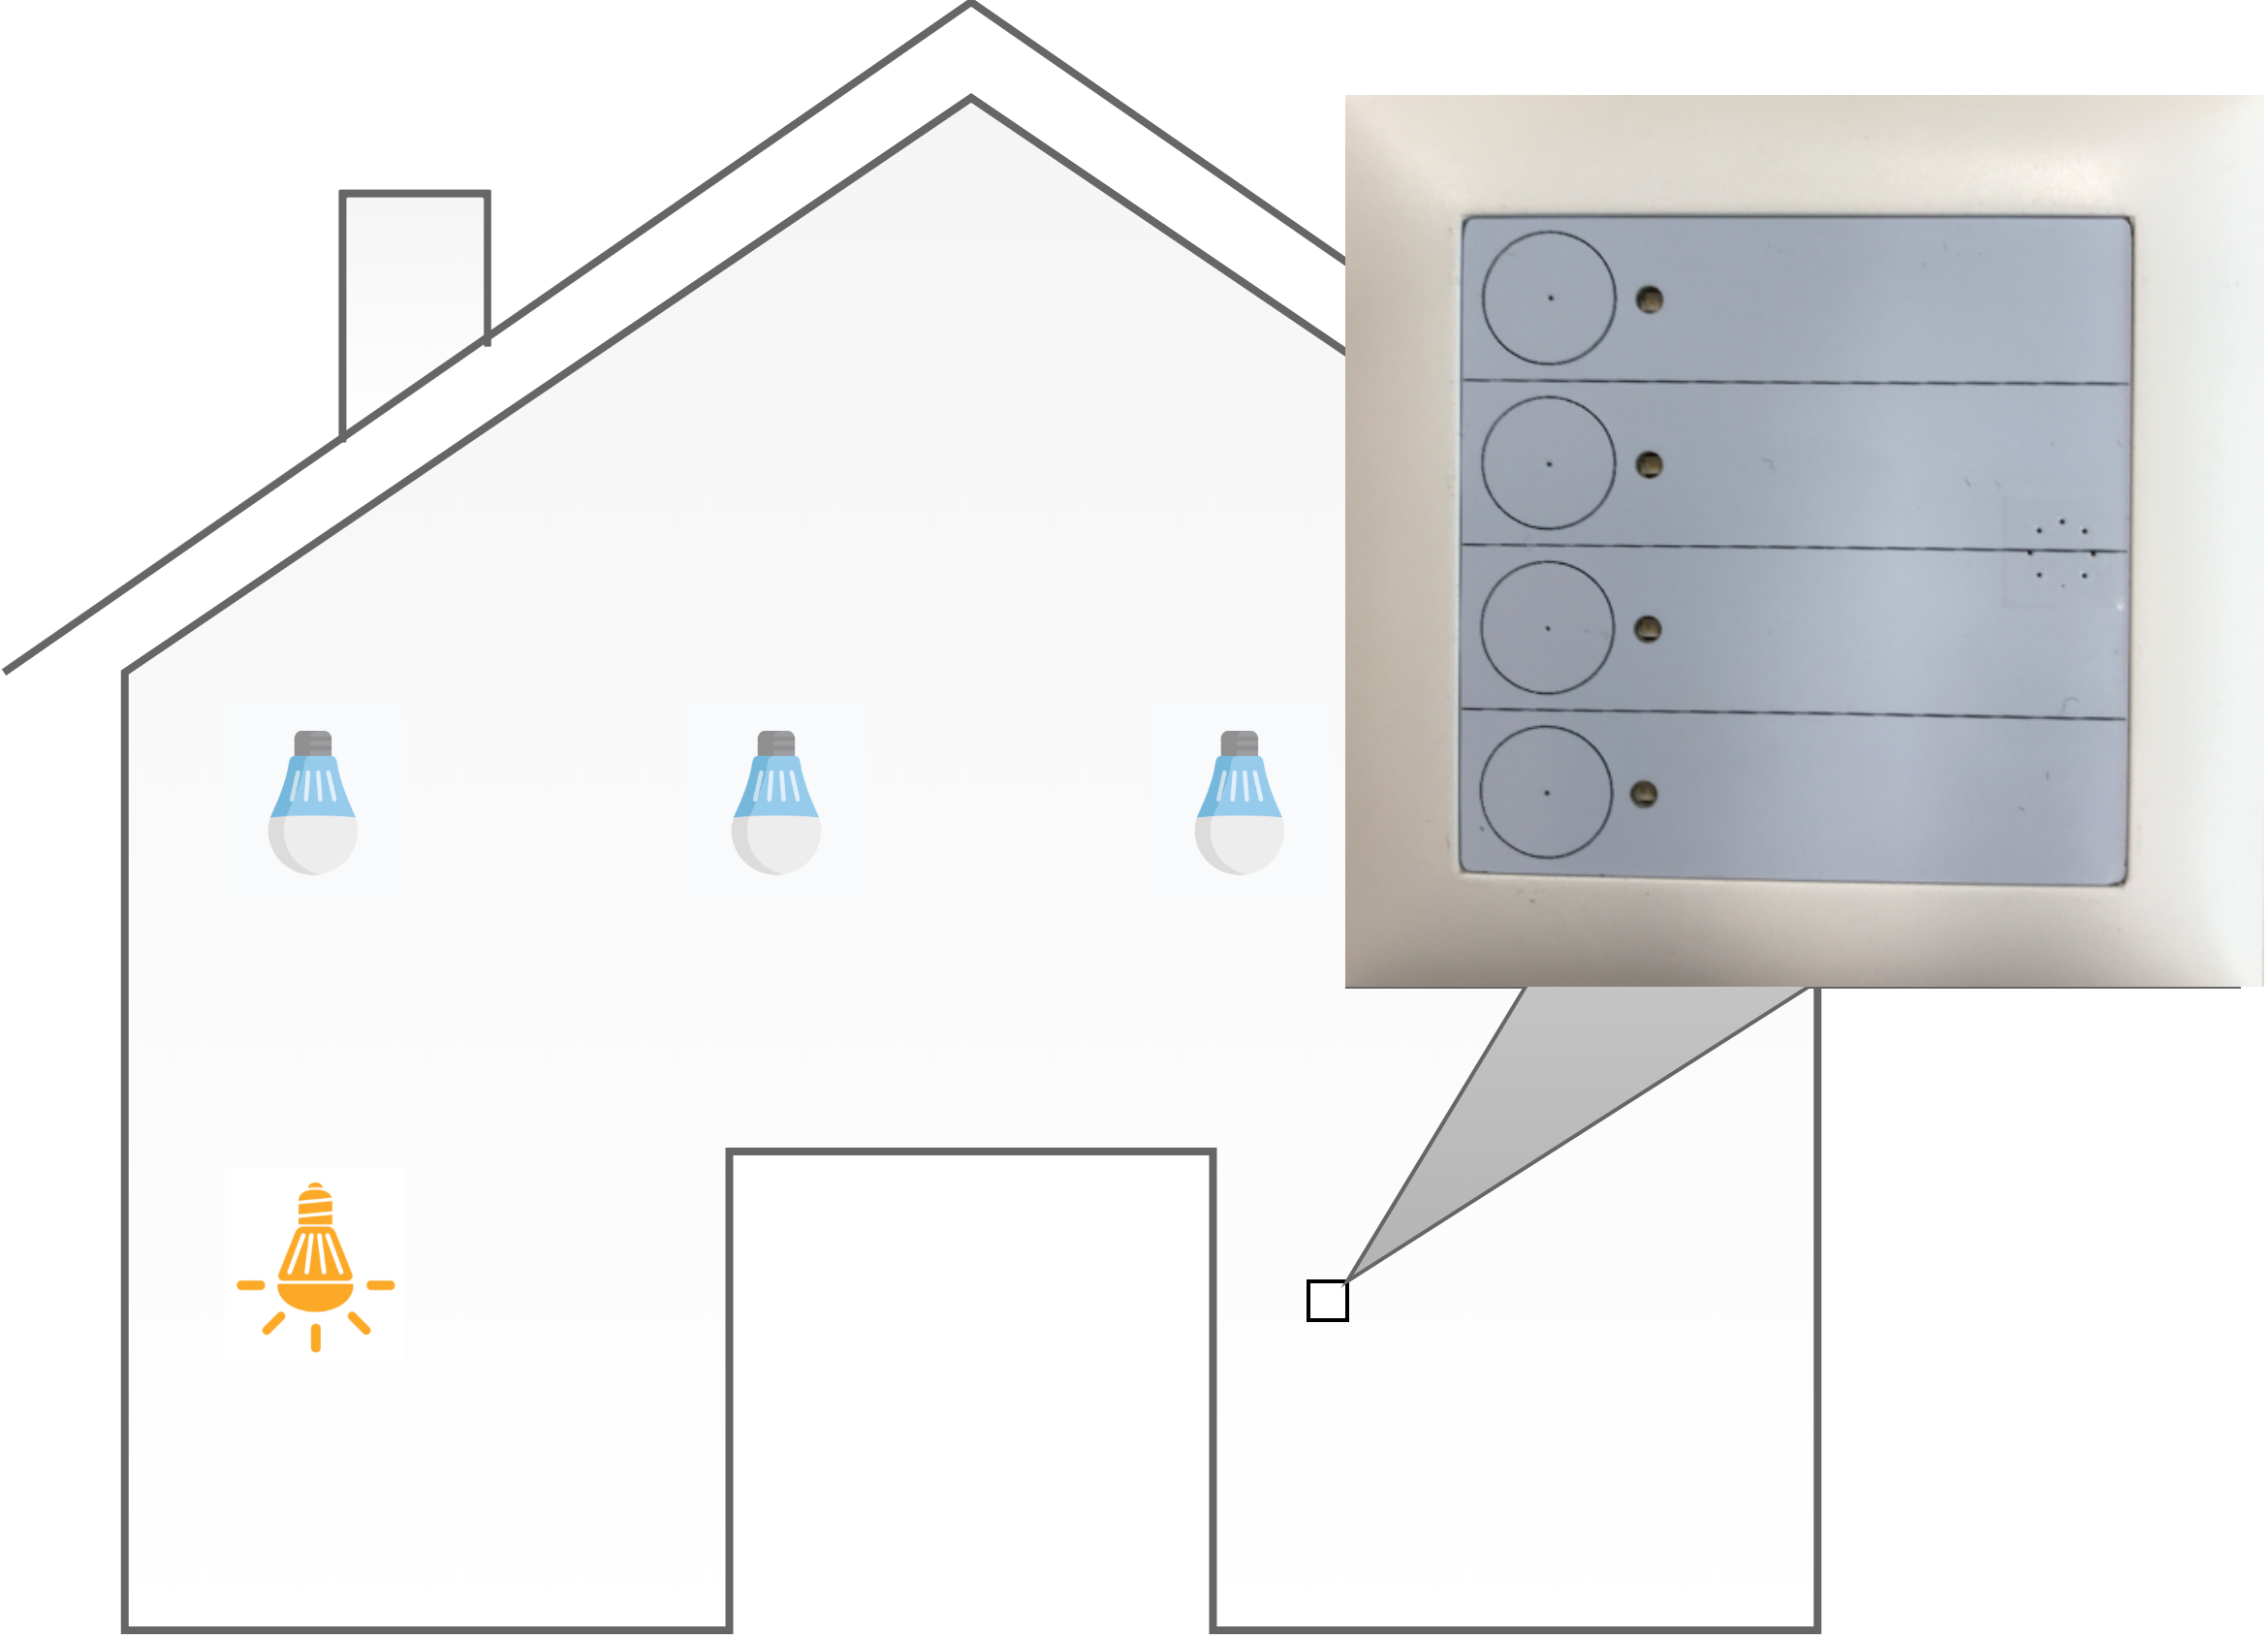
\includegraphics[width=\linewidth]{titelbild.png}
\end{figure}
\vfill

\begin{center}
\renewcommand\arraystretch{2}
\begin{tabular}{>{\bf}p{4cm} l}
Hochschule                 &    Hochschule für Technik - FHNW\\
Studiengang                &    Elektro- und Informationstechnik\\
Autoren   		                 & 	 Lukas Meienberger und Gabriel Nussbaumer\\
Betreuer                   &     Albert Zihlmann\\
Auftraggeber               &    Albert Zihlmann\\
Version                    &    1.0 %(Normally not used!)
\end{tabular}
\end{center}

\clearpage
			
%%---ABSTRACT----------------------------------------------------------------------------
\selectlanguage{ngerman}				%ngerman or english
\thispagestyle{empty}
\begin{abstract}

Smart Home is the automation, and data-based control of electronic devices and light energy systems in your own home. This report is about a smart home system solution with MQTT communication. The development of an actor board with different switching possibilities, where electronic devices are connected, as well as the development of a touch sensor board with temperature measurement are described. A closed system with its own MQTT-broker is completed with the server software.The server software enables a perfect interaction between the components and the integration of a language assistant. The whole system can be integrated with existing Smart Home and offers cross-platform compatibility with other solutions.


%Der Softwareteil befasst sich mit verschiedenen Komponenten, so wird ein Framework für den Sensor/Aktorbaustein wie auch das Framework für den Inhouse Server und das MQTT Konzept beschrieben. Das Hardwarekonzept des Sensorbausteins besteht im wesentlichen aus einem WiFi fähigen Mikrocontroller, einem Temperatursensor, Buttons und LEDs. Dabei besteht der Sensorbaustein aus drei physisch getrennten Teilen: der Spannungsversorgung, dem Hauptprint und der Frontprint. Der Frontprint beinhaltet Touchsensoren und LEDs, welche einen individualisierten Einschaltzustand, z.B Lüftung ist an, signalisieren. Das wichtigste im Aktorbaustein ist ebenso ein Mikrocontroller mit WiFi, dazu kommen noch Relais, $10\;V$ Ein-/Ausgänge und LEDs, um den Schaltzustand der Relais zu signalisieren.

%Das Abstract ist eine Art Zusammenfassung des ganzen Dokuments. Es gibt einen Einblick in die Aufgabenstellung, wie diese umgesetzt wurde und welches Ergebnis erreicht wurde. Aus diesem Grund wird das Abstract immer ganz am Schluss der Arbeit verfasst. Es besteht aus einem zusammengehörenden Absatz und umfasst ungefähr 10 bis 20 Zeilen.Formeln, Referenzen oder andere Unterbrechungen haben im Text nichts zu suchen.Direkt unter dem Abstract folgt eine Liste von drei bis vier Stichworten/Keywords. Diese werden in alphabetischer Reihenfolge aufgelistet und beschreiben das Themengebiet der Arbeit.

%\vspace{2ex}
%\textbf{Keywords: Anleitung, LaTeX, Thesis, Vorlage}
\end{abstract}	

%%---TABLE OF CONTENTS-------------------------------------------------------------------
\pagenumbering{Roman}		
\selectlanguage{ngerman}				%ngerman or english
\tableofcontents
\clearpage

%%---TEXT--------------------------------------------------------------------------------
\pagenumbering{arabic}
\section{Einleitung} 
Für eine integrale Raumautomation müssen alle beteiligten Gewerke geregelt werden, dazu gehören: Beschattung, Licht, Heizung, Lüftung und Klima.
Der Auftraggeber möchte eine möglichst preisgünstige Sensor/Aktor-Plattform um jene integrale Raumautomation zu ermöglichen. Bisher wurde die Idee, verschiedene Sensoren und Aktoren über IOT miteinander auszulesen bzw. zu steuern, in der Raumautomations-Branche verwirklicht, jedoch hat es sich als schwierig erwiesen solch eine anwendungsfreundliche Plattform, wie sich der Auftraggeber gewünscht hat, käuflich zu erwerben. Um die Situation zu verbessern soll eine Plattform auf Basis eines Single-Chip-uC, welcher Ein- und Ausgänge sowie ein Sensor-Baustein beinhalten realisiert werden. Zusätzlich möchte man mithilfe eines MQTT-Brokers die IOT-Geräte verbinden. Die Erstinbetriebnahme der Plattform soll mit Hilfe eines Web-Interface ablaufen, wofür das Gerät erstmal als WiFi Access-Point auf startet. 
Die folgende Tabelle \ref{tab: Ausgangslage} fasst die Anforderungen an das System zusammen.
\begin{table}[h!]
	\centering
	\begin{tabular}{|c|l|}
		\hline
		\textbf{\begin{tabular}[c]{@{}c@{}}Aktor\\   Baustein\end{tabular}} & \begin{tabular}[c]{@{}l@{}}\textbullet 4 Relais Schaltspannung 230 V\\ \textbullet 2 Ausgänge 0-10 V\\ \textbullet 2 Eingänge 0-10 V\\ \textbullet Netzwerkschnittstelle\\ \textbullet 24 VDC Versorgungsspannung\end{tabular} \\ \hline
		\textbf{Sensor Baustein}                                            & \begin{tabular}[c]{@{}l@{}}\textbullet 4 Taster\\ \textbullet Netzwerkschnittstelle\\ \textbullet Geometrie: Standard Lichtschalter\\ \textbullet 5 VDC Versorgungsspannung\end{tabular}                                       \\ \hline
		\multicolumn{1}{|l|}{\textbf{Kommunikation}}                        & \begin{tabular}[c]{@{}l@{}}\textbullet MQTT Broker\\ \textbullet WEB Interface\\
		\textbullet Sprach Assistent\end{tabular}                                                                                                                                   \\ \hline
	\end{tabular}
	\caption{Ausgangslage}
	\label{tab: Ausgangslage}
\end{table}%EXAMPLE
\section{Gesamtübersicht}
\begin{figure}[H]
\centering
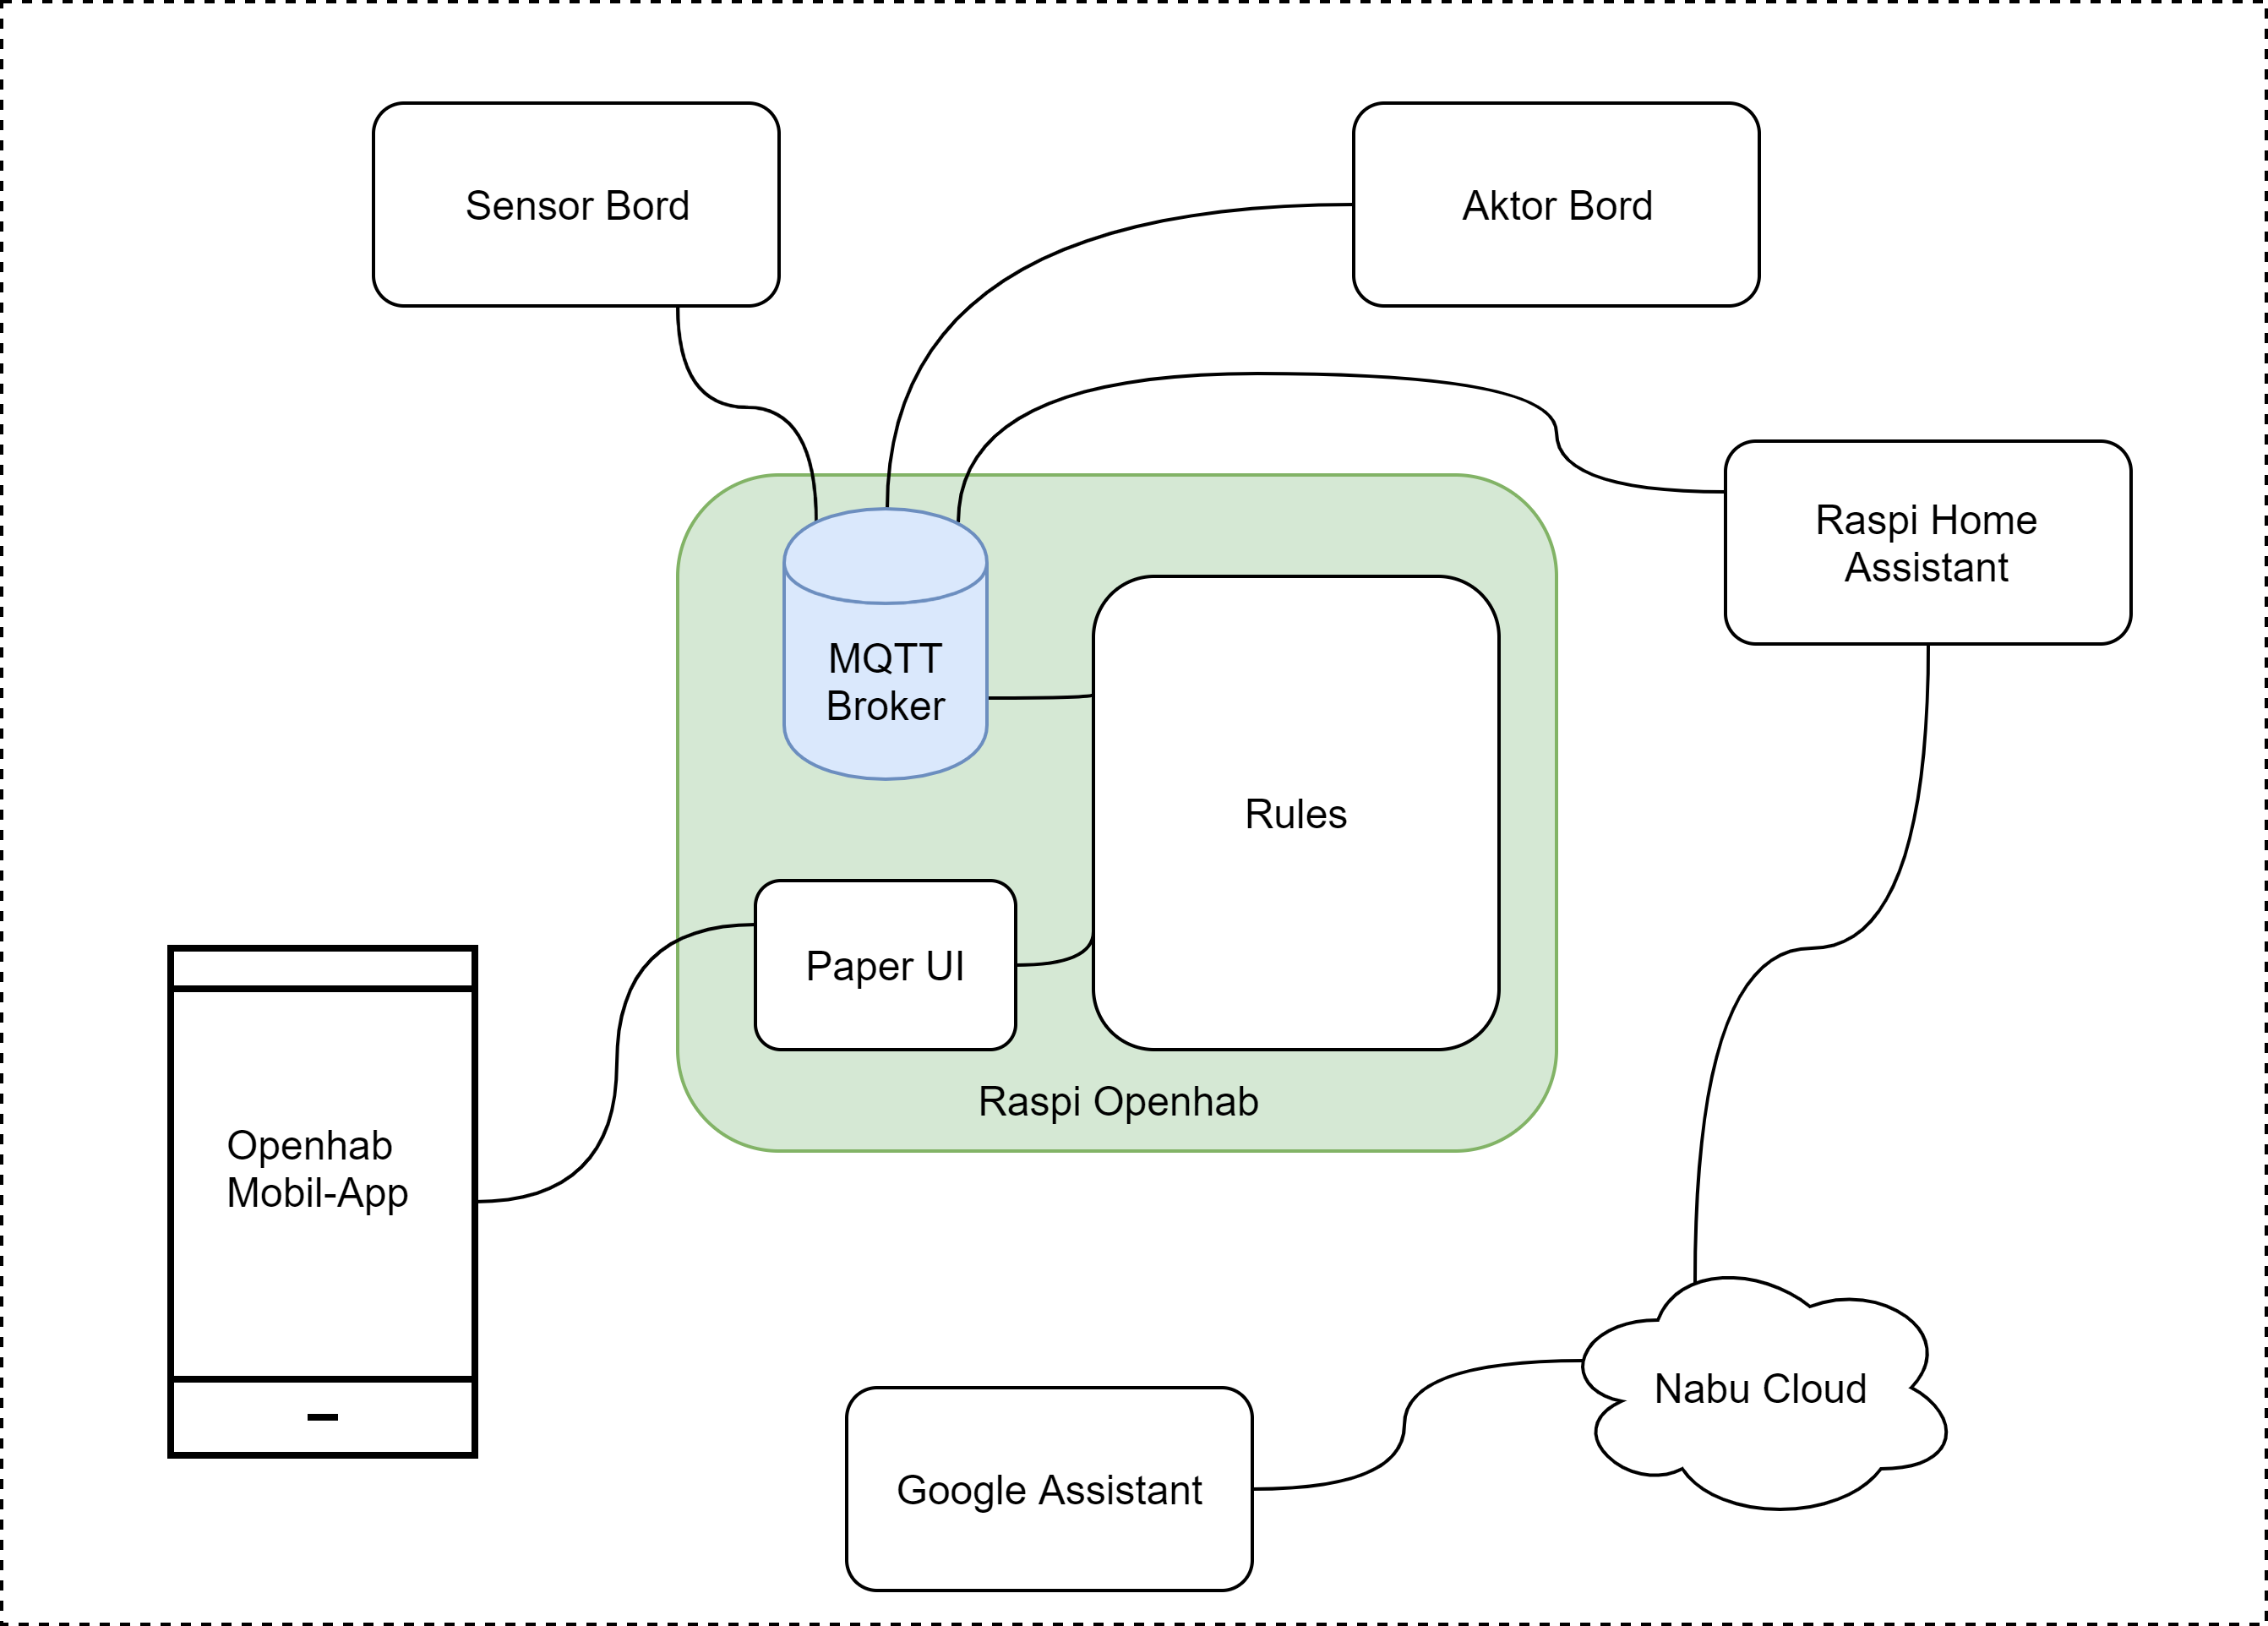
\includegraphics[width=\linewidth]{Gesammtubersicht.png}
\caption{Gesamtübersicht Komponenten Becholour Thesiss }
\label{pic: Gesamtübersicht}
\end{figure}
In der Abbildung \ref{pic: Gesamtübersicht} sind die Geräte und Ihre Verbindungen schematisch abgebildet. Als Herzstück dient der Openhab Server, welcher auf ein Rasperrypi aufgesetzt wurde. Ein eigener MQTT-Broker, welcher die Kommunikations-Messages managt wurde eingebunden. Verschiedene Geräte wie das Aktor- und Sensor-Board, auch der Home Assistant, welcher als Brücke für den Google Assistant dient, gelingt es im eigenen Lokalen Netzwerk zu kommunizieren. Als Web-Interface steht das Paper UI von Openhab wie auch das Mobile-App dem Benutzer, zum Bedienen vom System zur Verfügung. Mit den Rules sind alle automatisierten Vorgänge in Openhab festgelegt, in diesem Projekt sind dies die Definitionen bei welchem Befehl welche Schalthandlungen durchgeführt werden müssen. Der Grund warum die Schalthandlungen und die Verknüpfungen in den Ruls definiert werden, liegt daran, dass so keine Programmiereingriffe in die einzelnen Aktor- oder Sensor Boards Durchgeführt werden müssen. Der Benutzer kann die Konfigurationen in Openhab Graphisch im Web-Interface oder als Programmiercode in einem Editor wie Visual Studio Code durchführen, siehe im Anhang des Benutzerhandbuches.    





\section{Theorie}
\subsection{Wireless Local Area Network (WLAN)}
\subsubsection{Beschreibung}
Als lokales Funknetz ist WLAN weit verbreitet. WLAN ist eine Abkürzung für Wireless-Local-Area-Netzwerk, in deutsch ein Drahtloses-Lokales-Areal-Netzwerk. Die Idee der Lokalen Funkkommunikation war, dass in Büros mit mobilen Geräten wie Laptops eine Verbindung zum Internet hergestellt werden kann. Damit die Anbindung an das standardisierte LAN nicht in jedem Büro unterschiedliche Eigenschaften benötigt, wurde vom IEEE-Komitee entschieden ein Standard einzuführen, das Komitee entwickelte somit den 802.11 Standard für die drahtlosen Verbindungen. IEEE-802.11 Systeme nutzen unlizenzierte Frequenzbänder Bänder wie z.B. 902-928 MHz oder 2.4 - 2.5 GHz. Sämtliche Geräte dürfen dieses Spektrum nutzen, vorausgesetzt sie begrenzen ihre Sendeleistung, damit mehrere Geräte nebeneinander betrieben werden können. IEEE-802.11 Netze bestehen aus Clients wie Laptops und Smartphones sowie einer Infrastruktur, Zugangspunkt AP (Access Point), welcher im Gebäude Installiert ist. Der AP ist die Schnittstelle zum verkabelten Netz und ist im Privaten Haushalt auch oft direkt im Modem nebst dem Router integriert siehe Abbildung \ref{pic: IEEE802.11}.


 \begin{figure}[H]
	\centering
	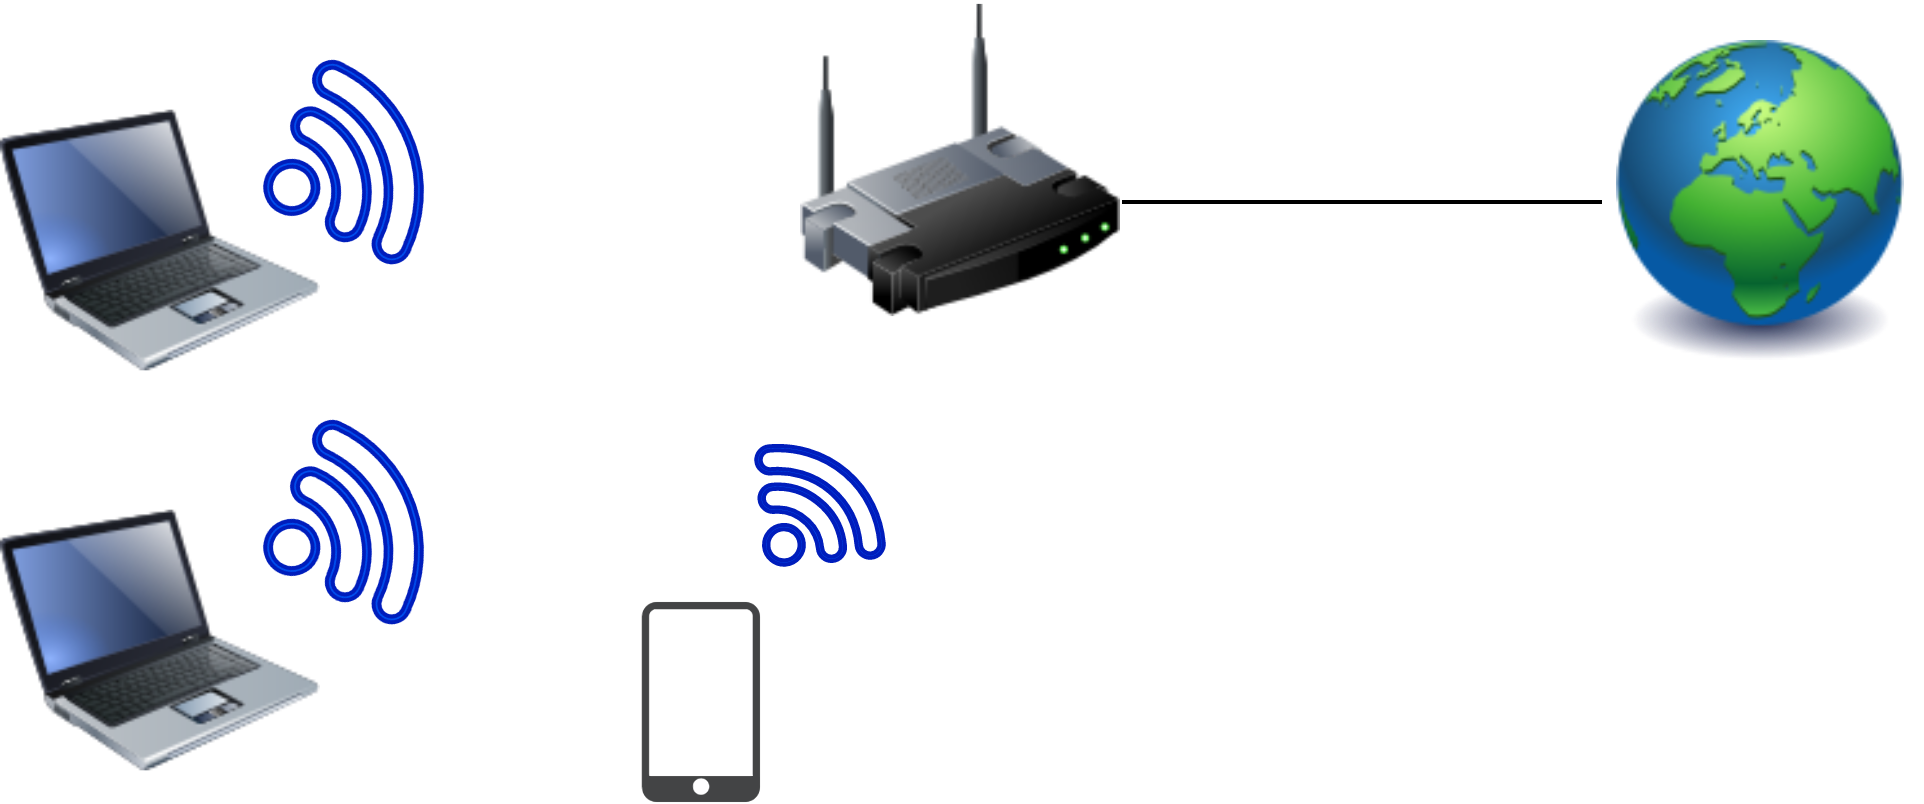
\includegraphics[width=\textwidth]{graphics/IEEE80211.png}
	\caption{Übersicht IEEE 802.11} 	
	\label{pic: IEEE802.11}
\end{figure} 
\subsubsection{Datenrate}
Der IEEE 802.11 Standard definierte 1997 ein drahtloses LAN, das entweder 1 Mbit/s oder 2 Mbit/s sendete und entweder Frequenzen wechselte oder das Signal über das erlaubte Spektrum verstreute. Die Funkverbindung wurde weiterentwickelt, so dass die Geschwindigkeit zunahm, in der nachfolgenden Tabelle ist eine Übersicht.
\begin{table}[H]
	\centering
	\begin{tabular}{|c|c|c|}
		\hline 
		Standard & Übertragungsleistung & Modulation \\ 
		\hline 
		IEEE-802.11b & 11Mbit/s & Frequenzspreizung \\ 
		\hline 
		IEEE-802.11a/g & 54Mbit/s & OFDM \\ 
		\hline 
		IEEE-802.11n & 450Mbit/s & Mehrerere Frequenzbänder \\ 
		\hline 
	\end{tabular} 
\caption{IEEE 802.11 Standarts \cite{wetherall_computernetzwerke_2012}}
\label{tab: IEEE802.11Standartds}
\end{table}
Das OFDM-Schema, Orthogonal Frequency Division Multiplexing, verwendet mehrere Trägerfrequenzen. Mehrere eng beieinanderliegende orthogonale Hilfsträgersignale mit überlappende Spektren übertragen Daten parallel.

\subsubsection{Sicherheit}

Die kabellosen Übertragungen sind Broadcast-Verbindungen, daher besteht das Problem, dass Informationspakete abgefangen werden können. Um dies zu verhindern ist im IEEE  802.11 Standard das Verschlüsselungsschema, WEP (Wired Equivalent Privacy) enthalten. Das WEP wurde durch WPA (WiFi Protected Access) ersetzt, und schliesslich wurde WPA durch WPA2 ersetzt. Im Juni 2018 wurde von Wi-Fi Alliance WPA3 vorgestellt, die nächste Generation der WiFi Sicherheit.\\
\\
\subsubsection{Funktion WPA2}

Die WPA2 Verschlüsselung wird in zwei verschiedenen Szenarien verwendet.\\
Ein Unternehmen hat ein Authentifizierungsserver mit Benutzernamen und Kennwortdatenbank eingerichtet, mit dem festgelegt wird ab ein drahtloser Client auf das Netz zugreifen darf. In diesem Fall verwenden Clients Standardprotokolle, um sich zu authentifizieren.
Im zweiten Szenario haben alle Clients ein gemeinsames Passwort, die Verbindung wird ohne Authentifizierungsserver aufgebaut. Diese Methode wird oft in privaten Netzwerken angewendet. Der Hauptunterschied ist, dass beim Authentifizierungsserver jeder Client ein Schlüssel zur Datenverschlüsselung bekommt, beim gemeinsamen Passwort wird der Schlüssel bei jedem Client aus dem Passwort abgeleitet und ist daher weniger sicher.
Nach dem sich der Client mit dem Passwort ausgewiesen hat, geschieht ein 4-Pakete-Handshake, und somit werden weitere Schlüssel erstellt.  
\subsubsection{WPA2 im Vergleich zu WPA3}
Bei WPA3 gibt es wieder die 2 verschiedenen Betriebsarten.\\
WPA3-Personal bietet eine stabilere kennwortbasierte Authentifizierung, selbst wenn Benuzter Kennwörter ändern, SAE (Simultaneous Authentication of Equals), schützt den Benutzer stärker gegen Dritte, welche versuchen das Passwort zu erraten.\\
WPA3 Enterprise bietet kryptografischen Schutz mit der Stärke von 192 Bit, somit geeignet für sensible Daten von einem Finanzinstitut \cite{noauthor_wi-fi_nodate}.























\newpage
\subsection{Message Queuing Telemetry Transport (MQTT)}
\subsubsection{Beschreibung}
MQTT ist ein Nachrichtentransport Protokoll, mittels Client werden Nachrichten veröffentlicht und abonniert und mit dem MQTT-Server verwaltet. Anwendung findet MQTT im Bereich in eingeschränkten Umgebungen, wie Kommunikation von Maschine zu Maschine (M2M) und Internet der Dinge (IoT). Das Protokoll läuft über TCP/IP oder über andere Netzwerkprotokolle die verlustfreie bidirektionale Verbindungen bieten \cite{noauthor_mqtt-v5.0.pdf_nodate}. 

\subsubsection{Geschichte}
MQTT wurde 1999 von dr.Andy Stanford-Clark von IBM und Arlen Nipper von Arcom erfunden. Seit 2013 ist MQTT über die nicht gewinnorientierte Organisation OASIS als Protokoll des Internet der Dinge standardisiert \cite{noauthor_mqtt-v5.0.pdf_nodate}. .
\subsubsection{Überischt}
 \begin{figure}[H]
 	\centering
 	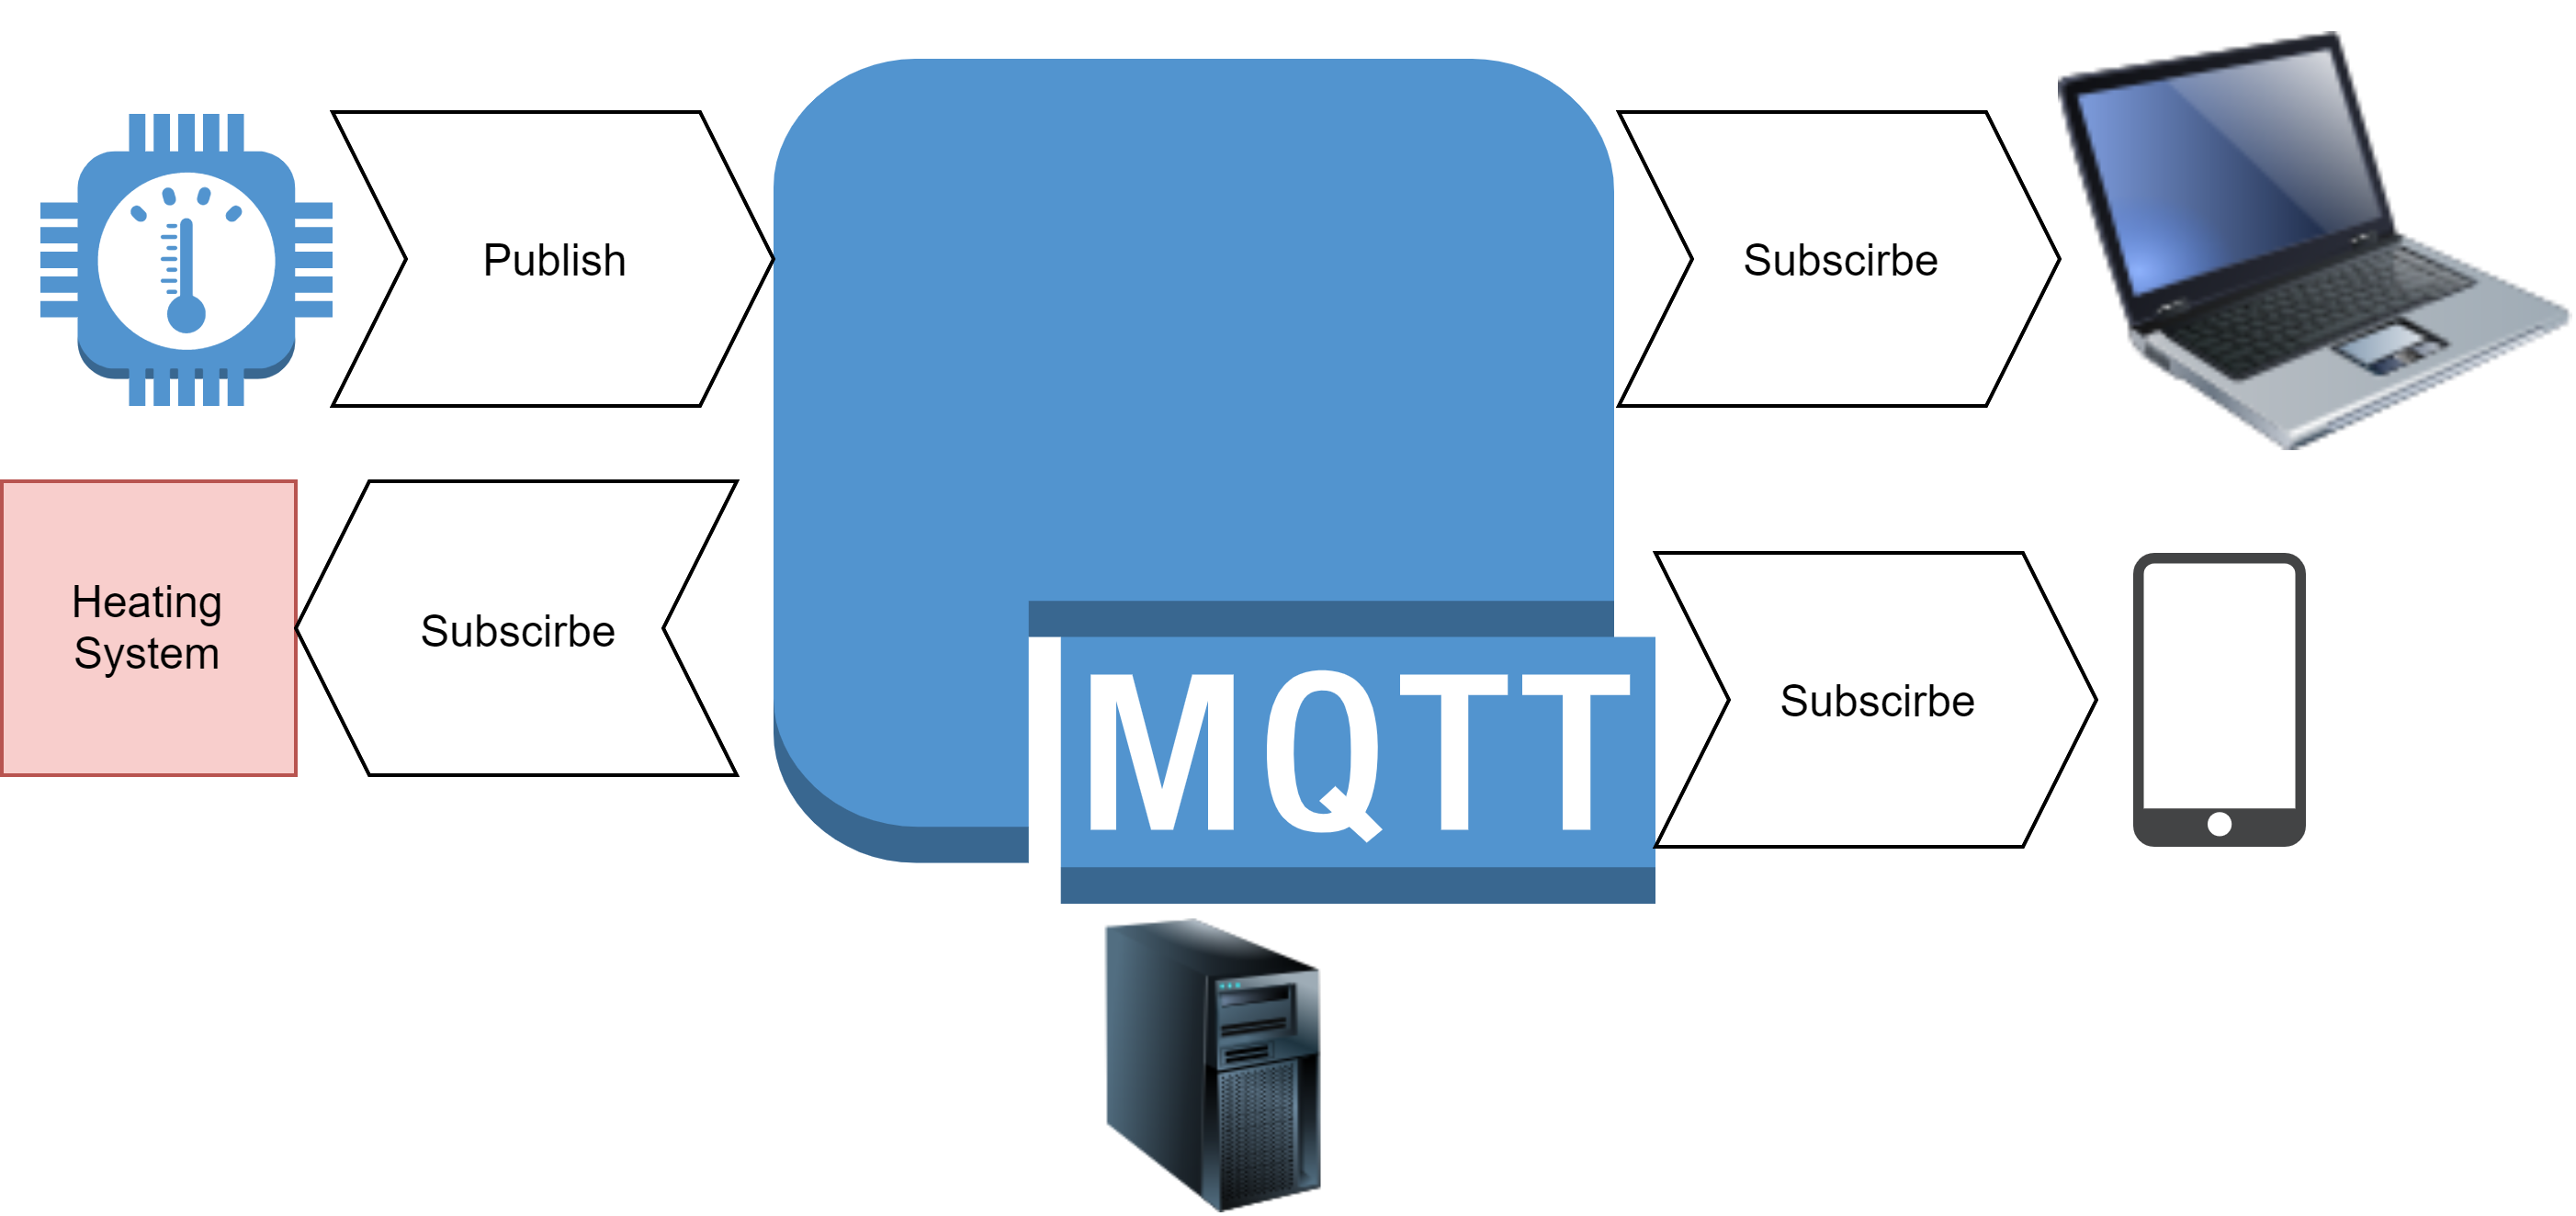
\includegraphics[width=\textwidth]{graphics/OverviewMQTT.PNG}
 	\caption{Übersicht MQTT} 	
 	\label{pic: OverMQTT}
 \end{figure} 
In der Abbildung \ref{pic: OverMQTT} werden Daten von einem Thermostat veröffentlicht. Ein Heizsystem, ein Notebook und ein Smartphone haben die Daten abonniert und der MQTT Brocker verwaltet die Nachrichten. 

\subsubsection{MQTT-Server (Brocker)}
Der MQTT-Server ist ein Programm oder Gerät, welches als Vermittler zwischen Clients dient und wird auch als MQTT-Broker bezeichnet. Der Broker nimmt Netzwerkverbindungen von Clients an, empfängt so die Nachrichten von Clients und gibt diese Nachrichten an jene Clients weiter, welche ein Abonnement abgeschlossen haben.

\subsubsection{Client}
Ein Client ist ein Programm oder Gerät, welches MQTT verwendet. Ein Client baut eine Verbindung zum Broker auf. Der Client veröffentlicht Nachrichten mit einem Topic und einem Inhalt. Ist ein Client an bestimmten Daten interessiert abonniert er diesen Topic und empfängt somit den Inhalt.
 
\subsubsection{Eigenschaften MQTT Brocker}
Veröffentlichen, abonnieren oder  Publish/Subscribe kann in Form von One-to-many Nachrichten verwendet werden.\\
MQTT benötigt wenig Zusatzinformationen beim Transport und minimiert so die Protokollaustausche, somit wird die Belastung des Netzwerkverkehrs minimiert.\\
Es gibt ein Mechanismus zur Benachrichtigung interessierter Parteien, wenn eine Unterbrechung einer Verbindung auftritt.\\
Für die Nachrichten Zustellung gibt es drei Service Qualitäten \cite{noauthor_mqtt-v5.0.pdf_nodate}:\\
\begin{itemize}
	\item Einmal übertragen, in diesem Fall wird die Nachricht, mit den besten Bemühungen der Betriebsumgebung, übermittelt.\\
		\item Mindestens einmal übertragen, wobei sichergestellt wird, dass die Nachricht ankommt, aber Duplikate auftreten können.\\
	\item Exakt einmal übermitteln, in diesem Fall wird sichergestellt, dass die Nachricht genau einmal ankommt.
\end{itemize}

\subsection{Mqtt Paket Struktur}
MQTT ist ein binärbasiertes Protokoll, bei dem die Steuerelemente Binäre Bytes sind, jedem Befehl ist eine Bestätigung zugeordnet.

\begin{figure}[H]
	\centering
	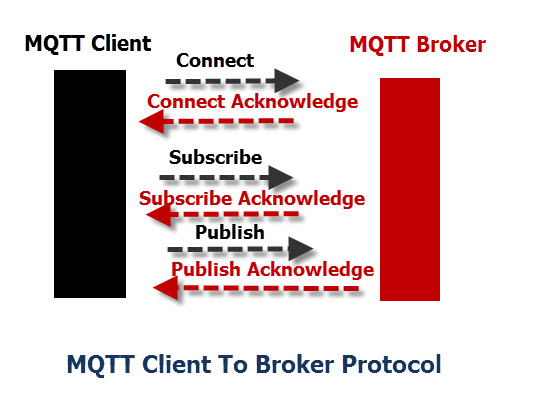
\includegraphics[width=\textwidth]{graphics/MQTTProtocolCommands.jpg}
	\caption{Bestätigung} 	
	\label{pic: OverMQTT}
\end{figure} 

\


\section{OpenHab}
In dieser Arbeit wird als Server ein RaspberryPi verwendet. Als Software befindet sich Openhab auf dem Linux Betriebssystem vom RaspberryPi. Openhab ist eine Gebäudeautomation Software und bietet Kontabilität zwischen verschiedenen Smarthome Komponenten wie KNX, Sonos, oder Philips Hue. Der für das Projekt benötigte MQTT Brocker kann als Binding in Openhab eingebunden werden. Nach den Installationen kann der funktionserhalt mit den Geräten im selben lokalen Netzwerk gewährleistet werden, auch ohne Verbindung mit dem öffentlichen Internet.
\subsection{Archidektur}
OpenHab basiert auf der modularen OSGI Architektur.
\subsubsection{OSGI}
Die OSGI Technologie bietet eine Vielzahl  von dynamischen Spezifikationen für Java Systemkomponenten. Dies ermöglicht ein Entwicklungsmodell, bei dem eine Anwendung aus  mehreren Komponenten Entsteht die als Pakete gebündelt sind. Die Komponenten sind Bausteine und sind wiederverwendbar, sie kommunizieren lokal untereinander. Die OSGI Architektur ermöglicht es den Komponenten die Implementierung vor andern Komponenten zu verbergen, während Dienste kommunizieren über Objekte gerade wenn sie von anderen Komponenten gemeinsam genutzt werden. Dies reduziert die Gesamtkomplexität und ermöglicht eine hohe Zuverlässigkeit, da während laufendem System Wartung und Entwicklungsarbeiten Durchführt werden können.  

%quelle: https://www.openhab.org/v2.2/docs/developer/prerequisites/osgi.html#bundles

 \begin{figure}[H]
	\centering
	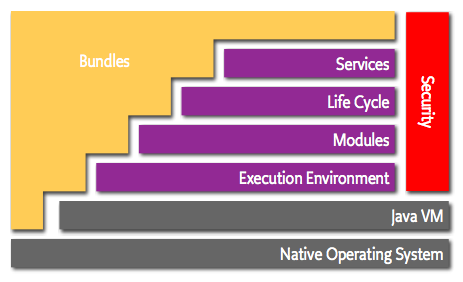
\includegraphics[width=\textwidth]{graphics/OSGI.png}
	\caption{OSGI Layers https://www.osgi.org/wp-content/uploads/layering-osgi.png} 	
	\label{pic: OSGILayers}
\end{figure} 

Bundles sind Module sie sind die kleinste Einheit der Modularisierung. Ein Bundle ist eine JAR-Datei mit zusätzlichen Meta-Informationen.\\
\\
In den Meta-Informationen sind Bundlesabhängigkeits Informationen. Ein Bundle kann von einem andern Bundel oder von einem Paket abhängig sein.\\
\\
Die OSGi-Runtime verwendet die Informationen über die Abhängigkeiten, um die Bundles zu verdrahten und versteckt alles in dieser JAR, sofern es nicht explizit exportiert wird. Die Abhängigkeiten zu den Java-Standardbibliotheken werden durch den Bundle-Header verwaltet, so dass es nicht notwendig ist, die Java-Kernpakete zu importieren.\\
\\
Bundles werden oft zur Registrierung und zum Konsum von Dienstleistungen verwendet.\\
\\
Die Bundles können in Laufzeit installiert, deinstalliert und geändert werden. Die Spezifikationen der OSGI Architektur also Abhängigkeiten und der Mechanismus wird mit Hilfe des Lebenszykluskonzepts erreicht. Der Rahmen führt verschiedene Zustände ein und regelt wie sich die vom Bundle exportierten Pakete und Dienste auswirken. 

 \begin{figure}[H]
	\centering
	\includegraphics[width=\textwidth]{graphics/BundleState.png}
	\caption{Bundle State Diagramm} 	
	\label{pic: BundleState}
\end{figure} 

In diesem Diagramm ist ersichtlich, dass Bundles während des Ausführens nicht geändert werden können, sonnst aber jederzeit.

\subsubsection{JAR}
\subsubsection{Übersicht Kommunikation Verbindungen}
Die Kommunikation zwischen den Komponenten geschieht mittels Event Bus. Alle nicht statusbezogenen Bundels informieren darüber andere Bundles über den Status von Events. Über diesen Bus Kommunizieren alle Binding mit einem phsikalischen Link zur realen Hardware. Mit dem Events werden auf asynchrone weise in diesem Bus veröffentlicht, durch den EventSubscriber definierte Callback-Schnittstellen werden diese zur entsprechender Funktion vorgesehenen Events wiederum Empfangen. Der EventSubsciber ist als OSGI Dienst registriert \cite{noauthor_event_nodate}.

https://www.openhab.org/docs/developer/utils/events.html
   
  \begin{figure}[H]
 	\centering
 	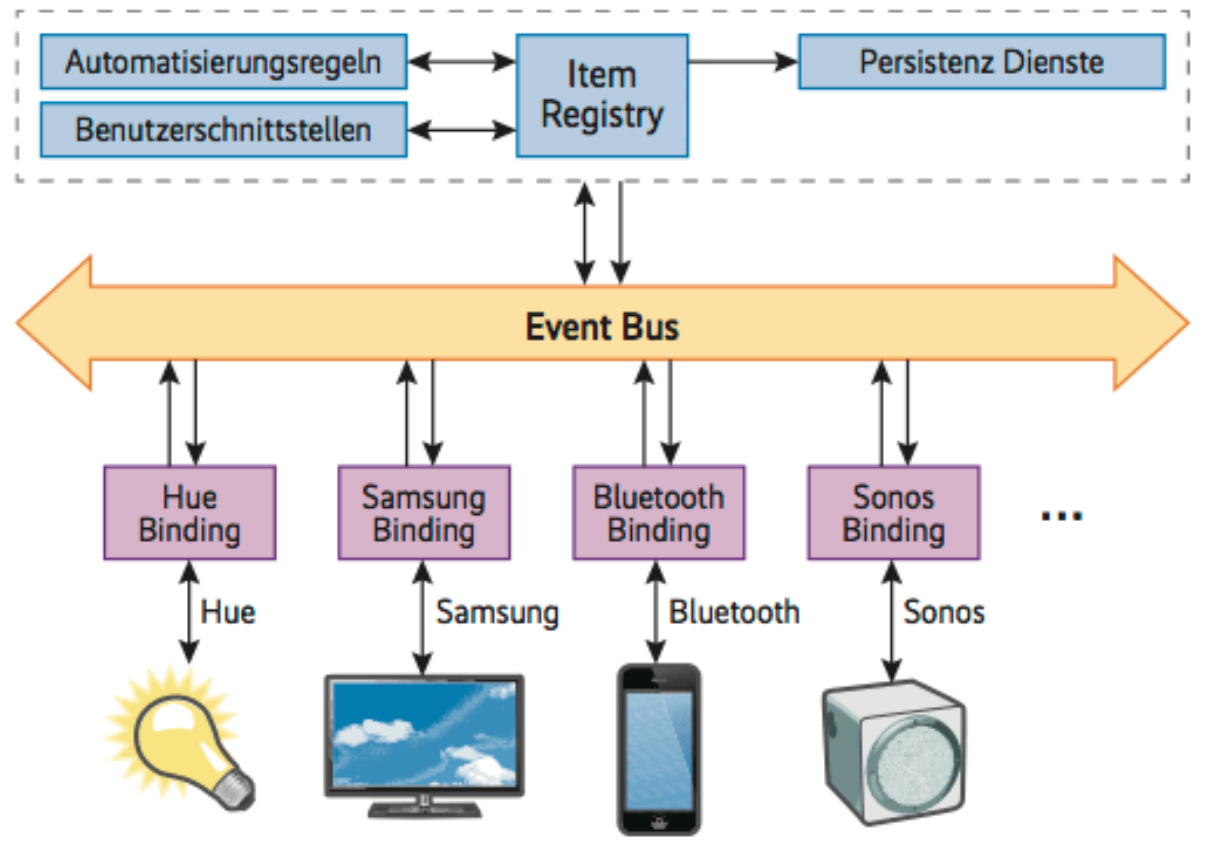
\includegraphics[width=\textwidth]{graphics/Eventbus.PNG}
 	\caption{Eventbus Openhab https://www.innoq.com/de/articles/2014/11/durchbruch/} 	
 	\label{pic: Eventbus}
 \end{figure} 
 
 In der Abbildung \ref{pic: Eventbus} ist der Eventbus dargestellt verschiedene Bindings mit Hardwarekomponenten von verschiedenen Smarthome lösungen empfange, die für sie vorgesehene Events
\section{Software}
In diesem Kapitel wird der Softwarebereich beschrieben. Es wird erklärt, wie die Frameworks der Mikrocontroller, welche auf den Sensor und Aktorbausteinen laufen, evaluiert wurden. Zusätzlich wird die Realisierung des Frameworks für den inhouse Server und die Kommunikation mit dem MQTT Protokoll aufgezeigt.

\subsection{Mikrocontroller}\label{subsec: Mikrocontroller}
Die Auswahl des Mikrocontrollers, ist so ausgefallen, dass dieser für Sensor wie auch für Aktor-Layout geeignet ist. Das Hauptkriterium der Wahl basiert auf der Kommunikation. Der Mikrocontroller von der chinesischen Firma Espressif Systems ist ein Robuster Chip, welcher für industrielle Umgebungen geeignet ist und in Betriebstemperaturen von -40 °C bis +125 °C zuverlässig arbeitet. Der Stromverbrauch kann zwischen verschiedenen Leistungsmodi gewählt werden, so kann während dem Betrieb eine dynamische Leistungsskalierung bewerkstelligt werden. ESP32 Module sind mit integrierten Antennen, Leistungsverstärkern und rauscharmen Empfangsverstärkern hochintegriert. Schnittstellen wie SPI, I2C, UART, WiFi und Bluetooth sind vorhanden.\\
WiFi:
Arbeitet mit dem Standart 802.11b/g/n und 802.11 2,4 GHz bis zu 150 Mbit/s. 4 Virtuelle Wi-Fi interfaces und Soft AP \\
Bluetooth:
Kompatibel mit Bluetooth v4.2 BR/EDR und BLE-Spezifikationen. Sender Klasse 1, Klasse 2 und Klasse 3 ohne externen Leistungsverstärker. Hochgeschwindigkeits-UART HCI, bis zu 4 Mbits/s.\\
CPU und Memory:
Modell abhängig, wobei das Modell ESP-WROOM-32E, mit der Chip Bezeichnung D0WD -V3 betrachtet wird. Dual-Core 32-bit, Flash 4-16 MB, 448 KB ROM, 520 KB SRAM, 16 KB SRAM in RTC. \\
Prozessor:
Tensilica Xtensa LX6 240 MHz\\
Clocks und Timers:
Interner 8 MHz-Oszillator mit Kalibrierung. Externer Quarzoszillator 2 MHz bis 40 MHz. Zwei Timer Gruppen 2x 64-bit Timer mit je einem Haupt Watchdog.\\
Erweiterte Peripherieschnittstellen:
12-bit SAR ADC bis zu 18 Kanäle, 2x b-bit D/A Wandler, 10x touch Sensoren, Temperatursensor, 4x SPI, 2x I2S, 2x I2C 3x UART.\\
Sicherheit:
Alle unterstützten Sicherheitsfunktionen des IEEE 802.11-Standards, einschließlich WFA, WPA/WPA2 und WAPI\\
Unterstützung bei der Entwicklung:
SDK Firmware für schnelle on-line Programmierung und open Source toolchains basiert auf GCC.\\
Kosten bei Mouser:\\
356-ESP32WROOM-32D 3,71 CHF/Stück
\subsubsection{ADC}
Der ADC des ESP32 verhält sich nicht liniear, was zu Problemen führen kann. In der Grafik \ref{pic: ESP32_Kurve} ist zu erkennen, dass der ADC nur bei grösser als U = 0.17\,V und kleiner als 3\,V überhaupt brauchbar ist, dazu kommt, dass ab 2.5\,V der ADC nichtliniear ansteigt. Die Lösung, welche hier verwendet wurde, war eine Linearisierung im Bereich von  0.2\,V bis 2.5\,V was zu folgender Geradengleichung geführt hat: $Wert_{ADC} = 1253.1\cdot U - 218.54$. Die Daten stammen aus dem Internet. Diese ist somit mit Vorsicht zu bewerten, es wurden für den Sensor- und Aktorbaustein besser passende Geradengleichungen verwendet, eine für die Temperaturmessung und eine für die analogen Eingänge.
\begin{figure}[h!]
	\centering
	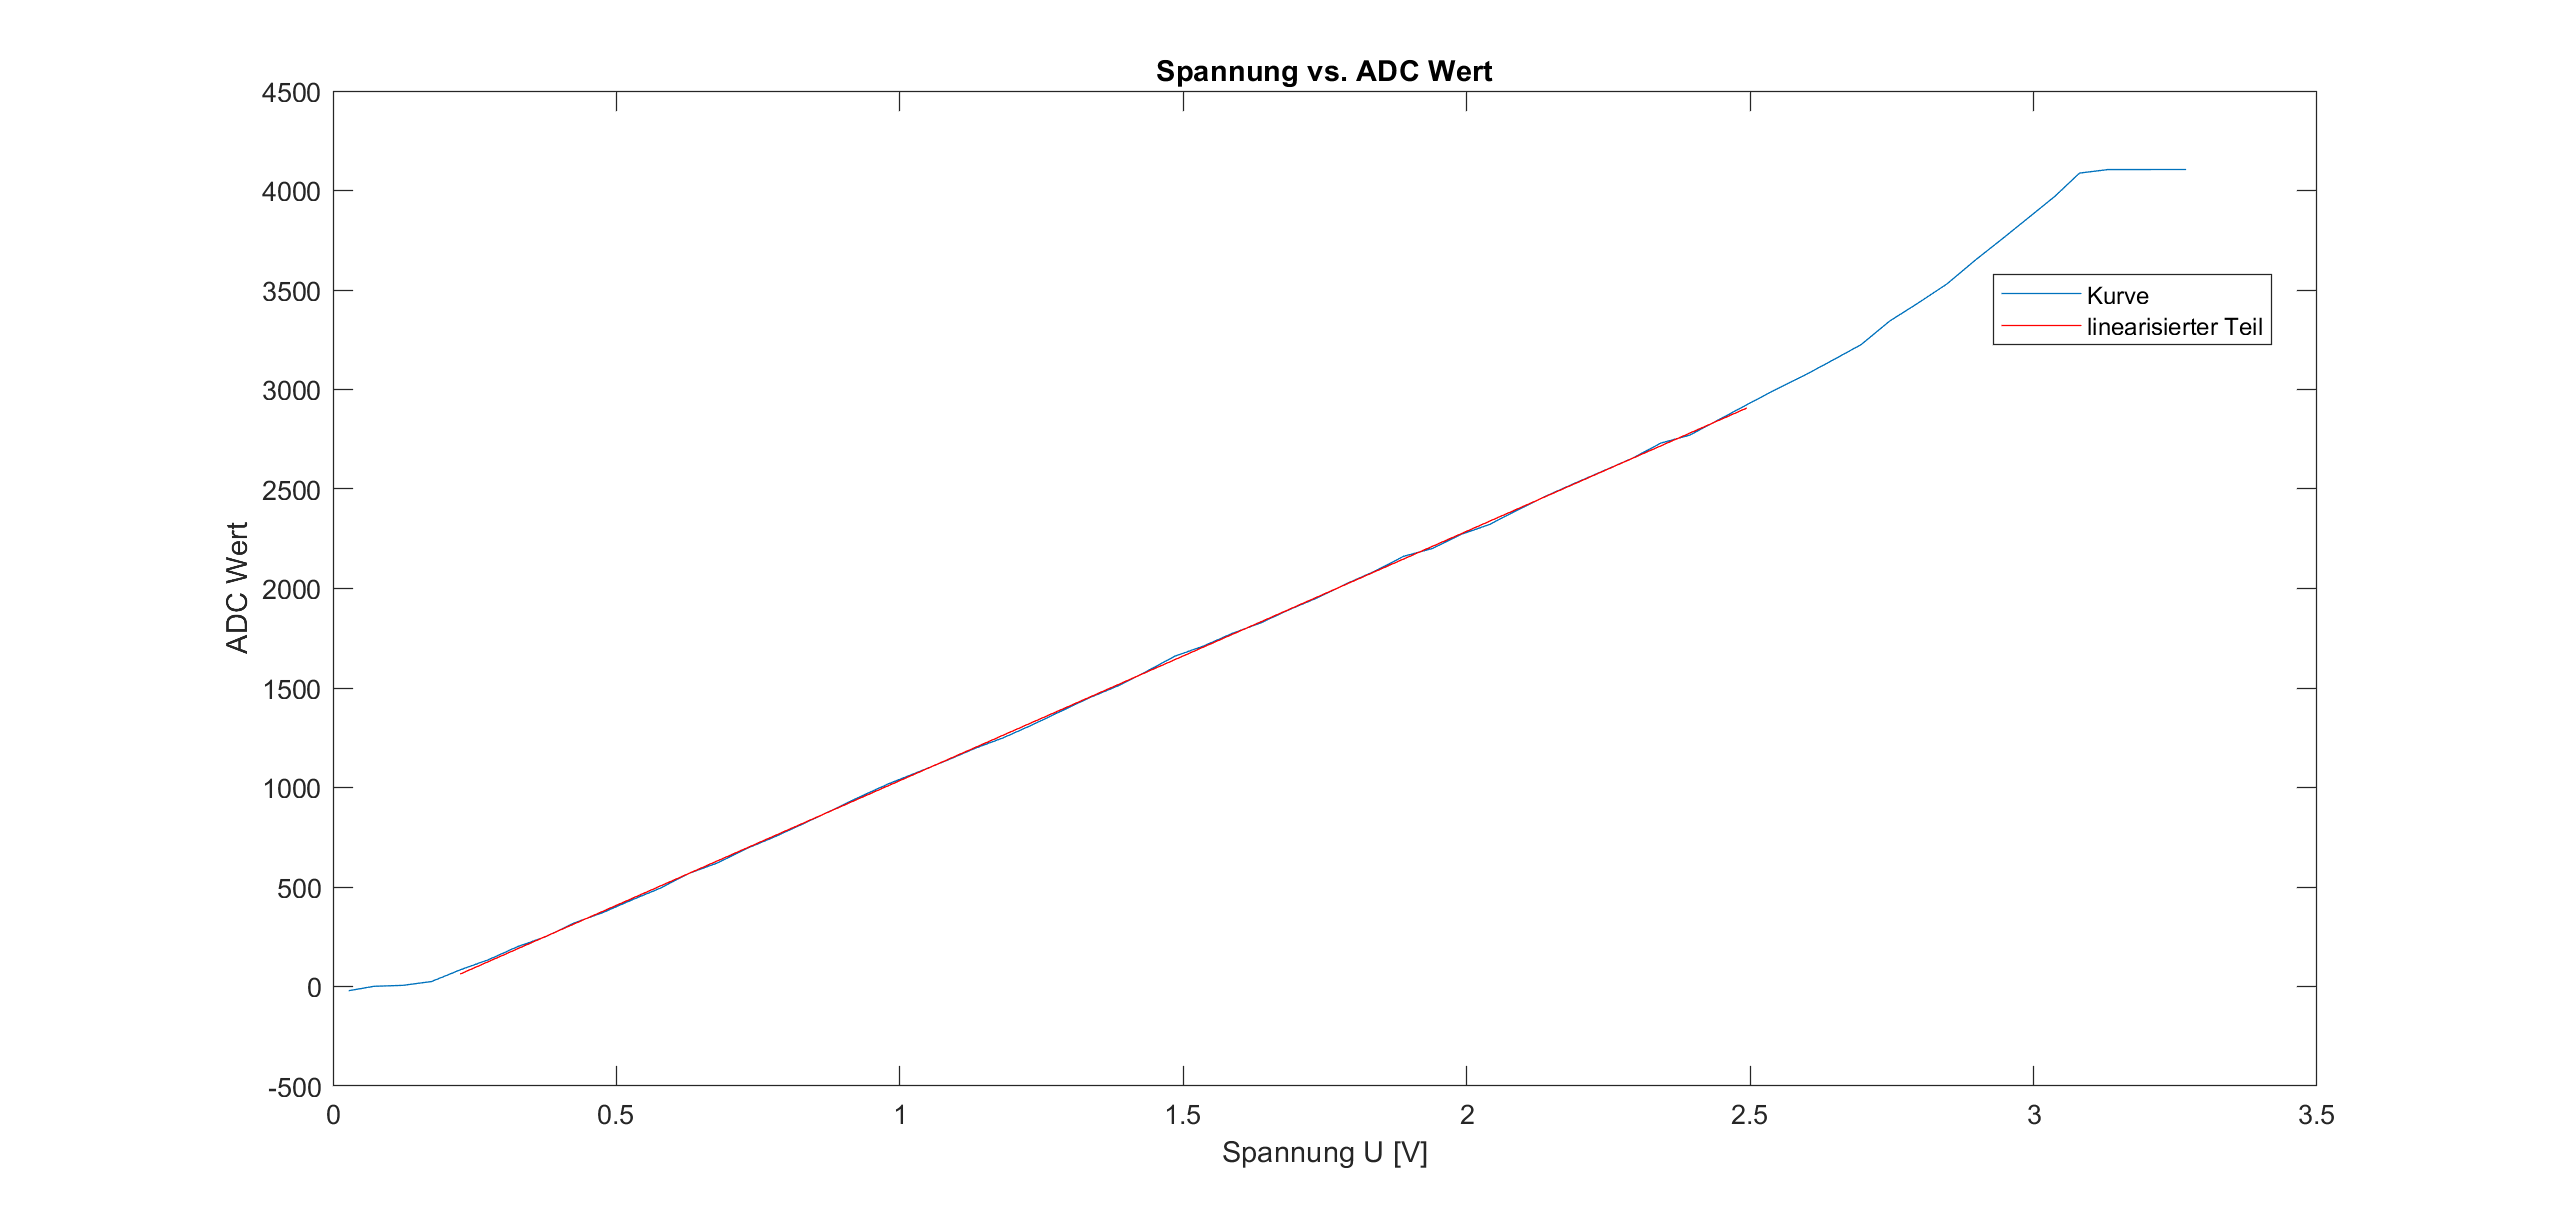
\includegraphics[width=\textwidth]{graphics/ESP32_Kurve.png}
	\caption{ESP32 Kurve, Daten aus Grafik von \cite{randomnerdtutorials_esp32_2019}}
	\label{pic: ESP32_Kurve}
\end{figure}


\newpage
\subsection{Framework}\label{subsec: Framework}

\subsubsection{Entwicklerumgebung} 
\begin{figure}[H]
	\centering
	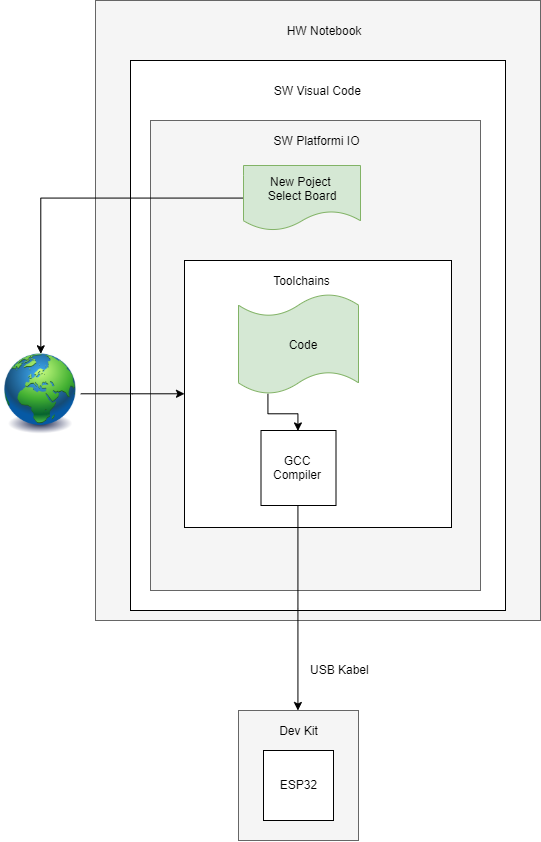
\includegraphics[width=0.8\textwidth]{graphics/DevelopDiagram.png}
	\caption{Entwicklungs Umgebung}
	\label{pic: PIO}
\end{figure} 

 Als Entwicklungsumgebung wird Visual Code von der Firma Microsoft verwendet, dies ist ein freier Quelltext-Editor, mit dem unter anderem Debugging möglich ist \cite{noauthor_visual_nodate}. In Visual Code können Extensions eingebunden werden, somit wird PlatformIO IDE \cite{platformio_platformio_nodate} kurz PIO Installiert und Openhab.
PIO ist ein plattformübergreifender Code Builder und Bibliotheksmanger. Wird ein neues Projekt eröffnet, muss vom Benutzer zuerst das Entwickler Board gewählt werden, anschliessend kümmert sich PIO um die erforderlichen Toolchains, ladet diese vom Internet herunter und installiert sie. Nun kann das Developmend-Board via USB Kabel angesprochen werden. Programmcode kann kompiliert und auf den Mikrocontroller geladen werden, die Serial Port ausgaben können direkt im PIO angezeigt werden. In Abbildung \ref{pic: PIO} ist ein Blockdiagramm auf dem die Verbindungen zwischen Software und Hardware dargestellt sind.

\subsubsection{Framework Arduino}
In dem Arduino Framework erfolgt die Programmierung in C und in C++ . Das Arduino Framework steht unter der LGPL/GPL Lizenz und ist somit eine freie Software. Ein grosser Vorteil des Arduino Frameworks ist, dass zahlreiche Bibliotheken und sowie Programmcode auf  Github erhältlich sind \cite{noauthor_arduino_nodate}.Die Wahl des Arduino Framwork ist auf Grund der Programmiersprache, Verfügbarkeit und bisherigen Erfahrungen erfolgt. Ein Funktionsmuster mit Hotspot, für Grundkonfigurationen und erste MQTT-Nachrichten, konnten Erfolgreich mit dem Arduino Framework realisiert werden.

\subsubsection{Smart-Home Plattform Openhab}
\label{subsubsec: Smart-Home Plattform}
Eine Smart-Home Plattform wird benötigt, damit der Benutzer mit dem IOT-Systems interagieren kann. 
Mit der Openhab Smart-Home-Plattform sind folgende Bedingungen erfüllt:\\
\begin{enumerate}
	\item Bietet Schnittstellen mit anderen Smart-Home Technologien wie KNX
	\item Benutzerfreundlich
	\item Client einsetzbar mittels verschiedenen Betriebssystemen
	\item Unabhängig vom öffentlichen Netz (Inhouse Server) 
\end{enumerate}
Openhab bietet sehr viele Schnittstellen, da durch den modularen Aufbau der Architektur die flexible Anbindung neuer Technologien einfach ist. Die für dieses Projekt wichtige Bindings von MQTT-Broker und KNX sind somit vorhanden. Was ebenso interessant ist, sind konfigurierbare Features wie Dropbox Support, und Google Kalender.
\newpage
\subsection{Kommunikation}\label{subsec: Kommunikation} 
\subsubsection{WLAN Konfiguration}\label{subsub: Wlan Konfiguration}
Die Funkkommunikation zwischen Sensor, Aktor und MQTT-Brocker wird mittels Wireless Local Area Network (WLAN) auf dem OSI layer 1 statt finden. Um die einzelnen Target also Sensoren und Aktoren in das Lokale Netzwerk zu verbinden, wird beim Starten des Mikrocontrollers ein Accespoint eröffnet. Für den Wifi-Configurations Prozess wird die entsprechende Bibliothek eingebunden. Diese steht auf Github zur Verfügung \cite{zhouhan0126_zhouhan0126/wifimanager-esp32_2019}. 

\begin{figure}[H]
	\centering
	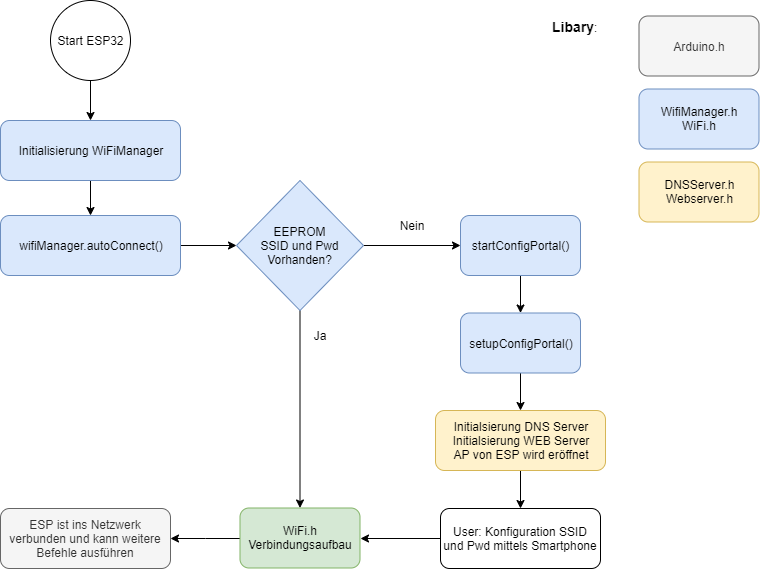
\includegraphics[width=\textwidth]{graphics/statediagramWiFi.png}
	\caption{Statediagram Verbindungsaufbau ESP ins Netzwerk mit einem AP}
	\label{pic: statediagramWiFi}
\end{figure}   

Wird die Bibliothek WiFiManager.h eingebunden und initialisiert stehen verschiedene Funktionen zur Verfügung. Die Funktion autoConnect() eröffnet nach dem Start des Mikrocontrollers einen Access-Point, wenn keine Konfigurationsdaten im nichtflüchtigen Speicher sind. Falls Konfigurationsdaten vorhanden sind, werden sie aus dem EEPROM gelesen und es wird kein Access-Point eröffnet.   

Mit einem Gerät beispielsweise Notebook oder Smartphone kann in den Netzwerk Einstellungen der Mikrocontroller mit dem Name 'Aktor' oder 'Sensor' mit anschliessender Chip-ID gefunden werden. 
Sobald "verbinden" mit diesem Netzwerk gewählt wird, startet der Webbrowser eine Konfigurationsseite. 

\begin{figure}[H]
	\centering
	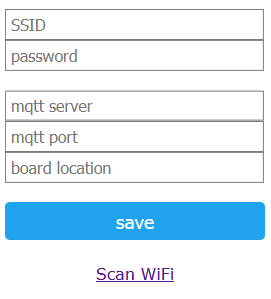
\includegraphics[width=0.3\textwidth]{graphics/Configportal2.PNG}
	\caption{Wifi Konfiguration Portal}
	\label{pic: Configportal}
\end{figure}   

Wird 'Scan Wifi' betätigt werden Netzwerke, welche in der Umgebung gefunden wurden, angezeigt, die Parameter die zur WiFi Verbindung notwendig sind, können nun eingegeben werden. Im unteren Teil wird die MQTT-Brocker-Adresse und der Port eingegeben. Als `board-location' soll der Standort des Gerätes eingegeben werden, aus dieser Eingabe werden MQTT-topics generiert. 

\begin{figure}[H]
	\centering
	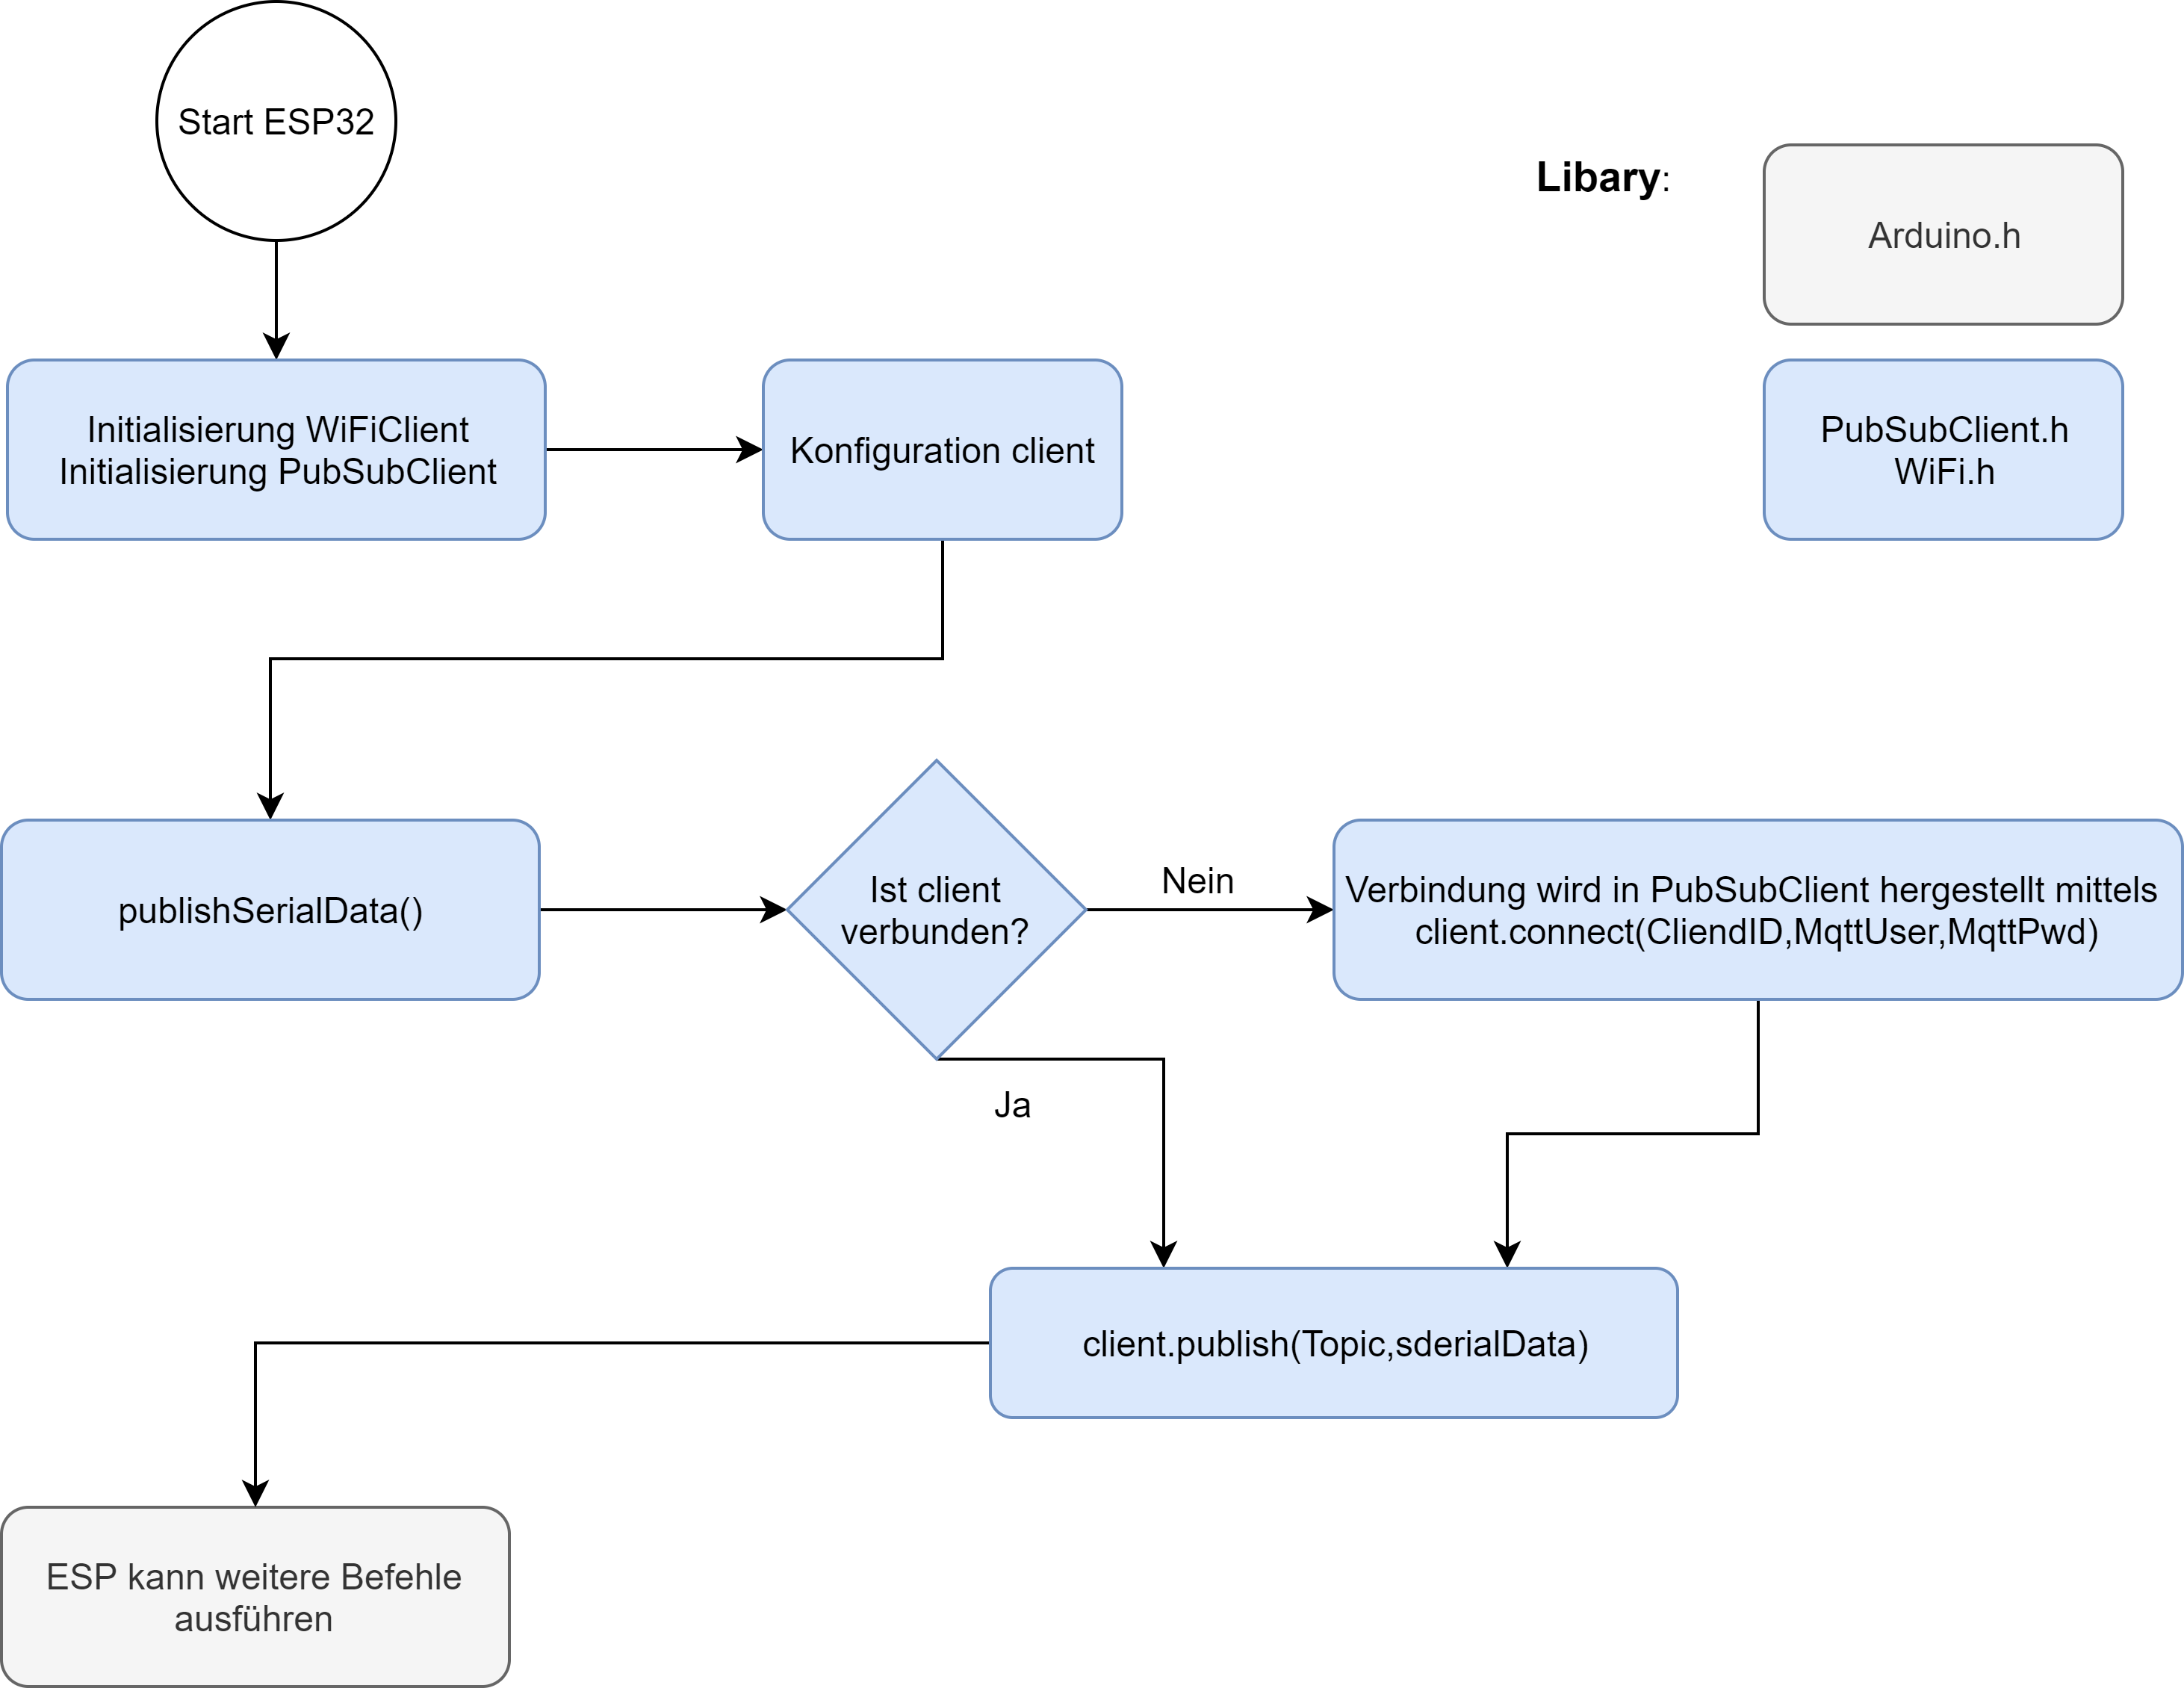
\includegraphics[width=\textwidth]{graphics/MQTTSubPubClient.png}
	\caption{Esp Info}
	\label{pic: SubPubClient}
\end{figure}   

Die für die MQTT-Kommunikation wird die Libary PubSubClient.h eingebunden. Als erstes wird der WiFiClient initialisiert. 

Danach wird der PubSubClinet als Client instanziiert, für diesen Vorgang werden folgende Parameter benötigt:\\
\begin{itemize}
\item 	server: Adresse von MQTT-Server\\
\item 	port: der Port von dem MQTT-Server\\
\item 	client: eine Instanz vom Ethernet-Client.\\
\end{itemize}
Die Funktion publishSerialData() ermöglicht, eine Nachricht zu veröffentlichen, bei diesem Vorgang wird den Topic und die Payload veröffentlicht. Beim Aufruf dieser Funktion, wird jedes mal überprüft ob die Verbindung zum MQTT-Broker in Ordnung ist. 

Ist die Verbindung nicht in Ordnung, wird sie mit der Funktion reconnect() hergestellt.

Ist die Verbindung in Ordnung werden die Daten mit dem Befehl publish() veröffentlicht \cite{noauthor_arduino_nodate-1}.

\subsection{Programmcode Sensorbord}
Die Aufgabe welcher der Mikrocontroller vom Sensorboard  übernehmen besteht darin, dass er Betätigungen der Touchtasten auf dem Frontprint erkennt. Jeder Touchtaster besitzt ein LED mit dem das Betätigen bestätigt wird. Diese Funktion wurde so initialisiert, damit der User eine sofortige Kenntnis über die ausgelöste Aktion bekommt. Mit dem Sensorboard wird auf dem Frontprint die Umgebungstemperatur gemessen.



\subsubsection{	Übersicht} 
\begin{figure}[H]
	\centering
	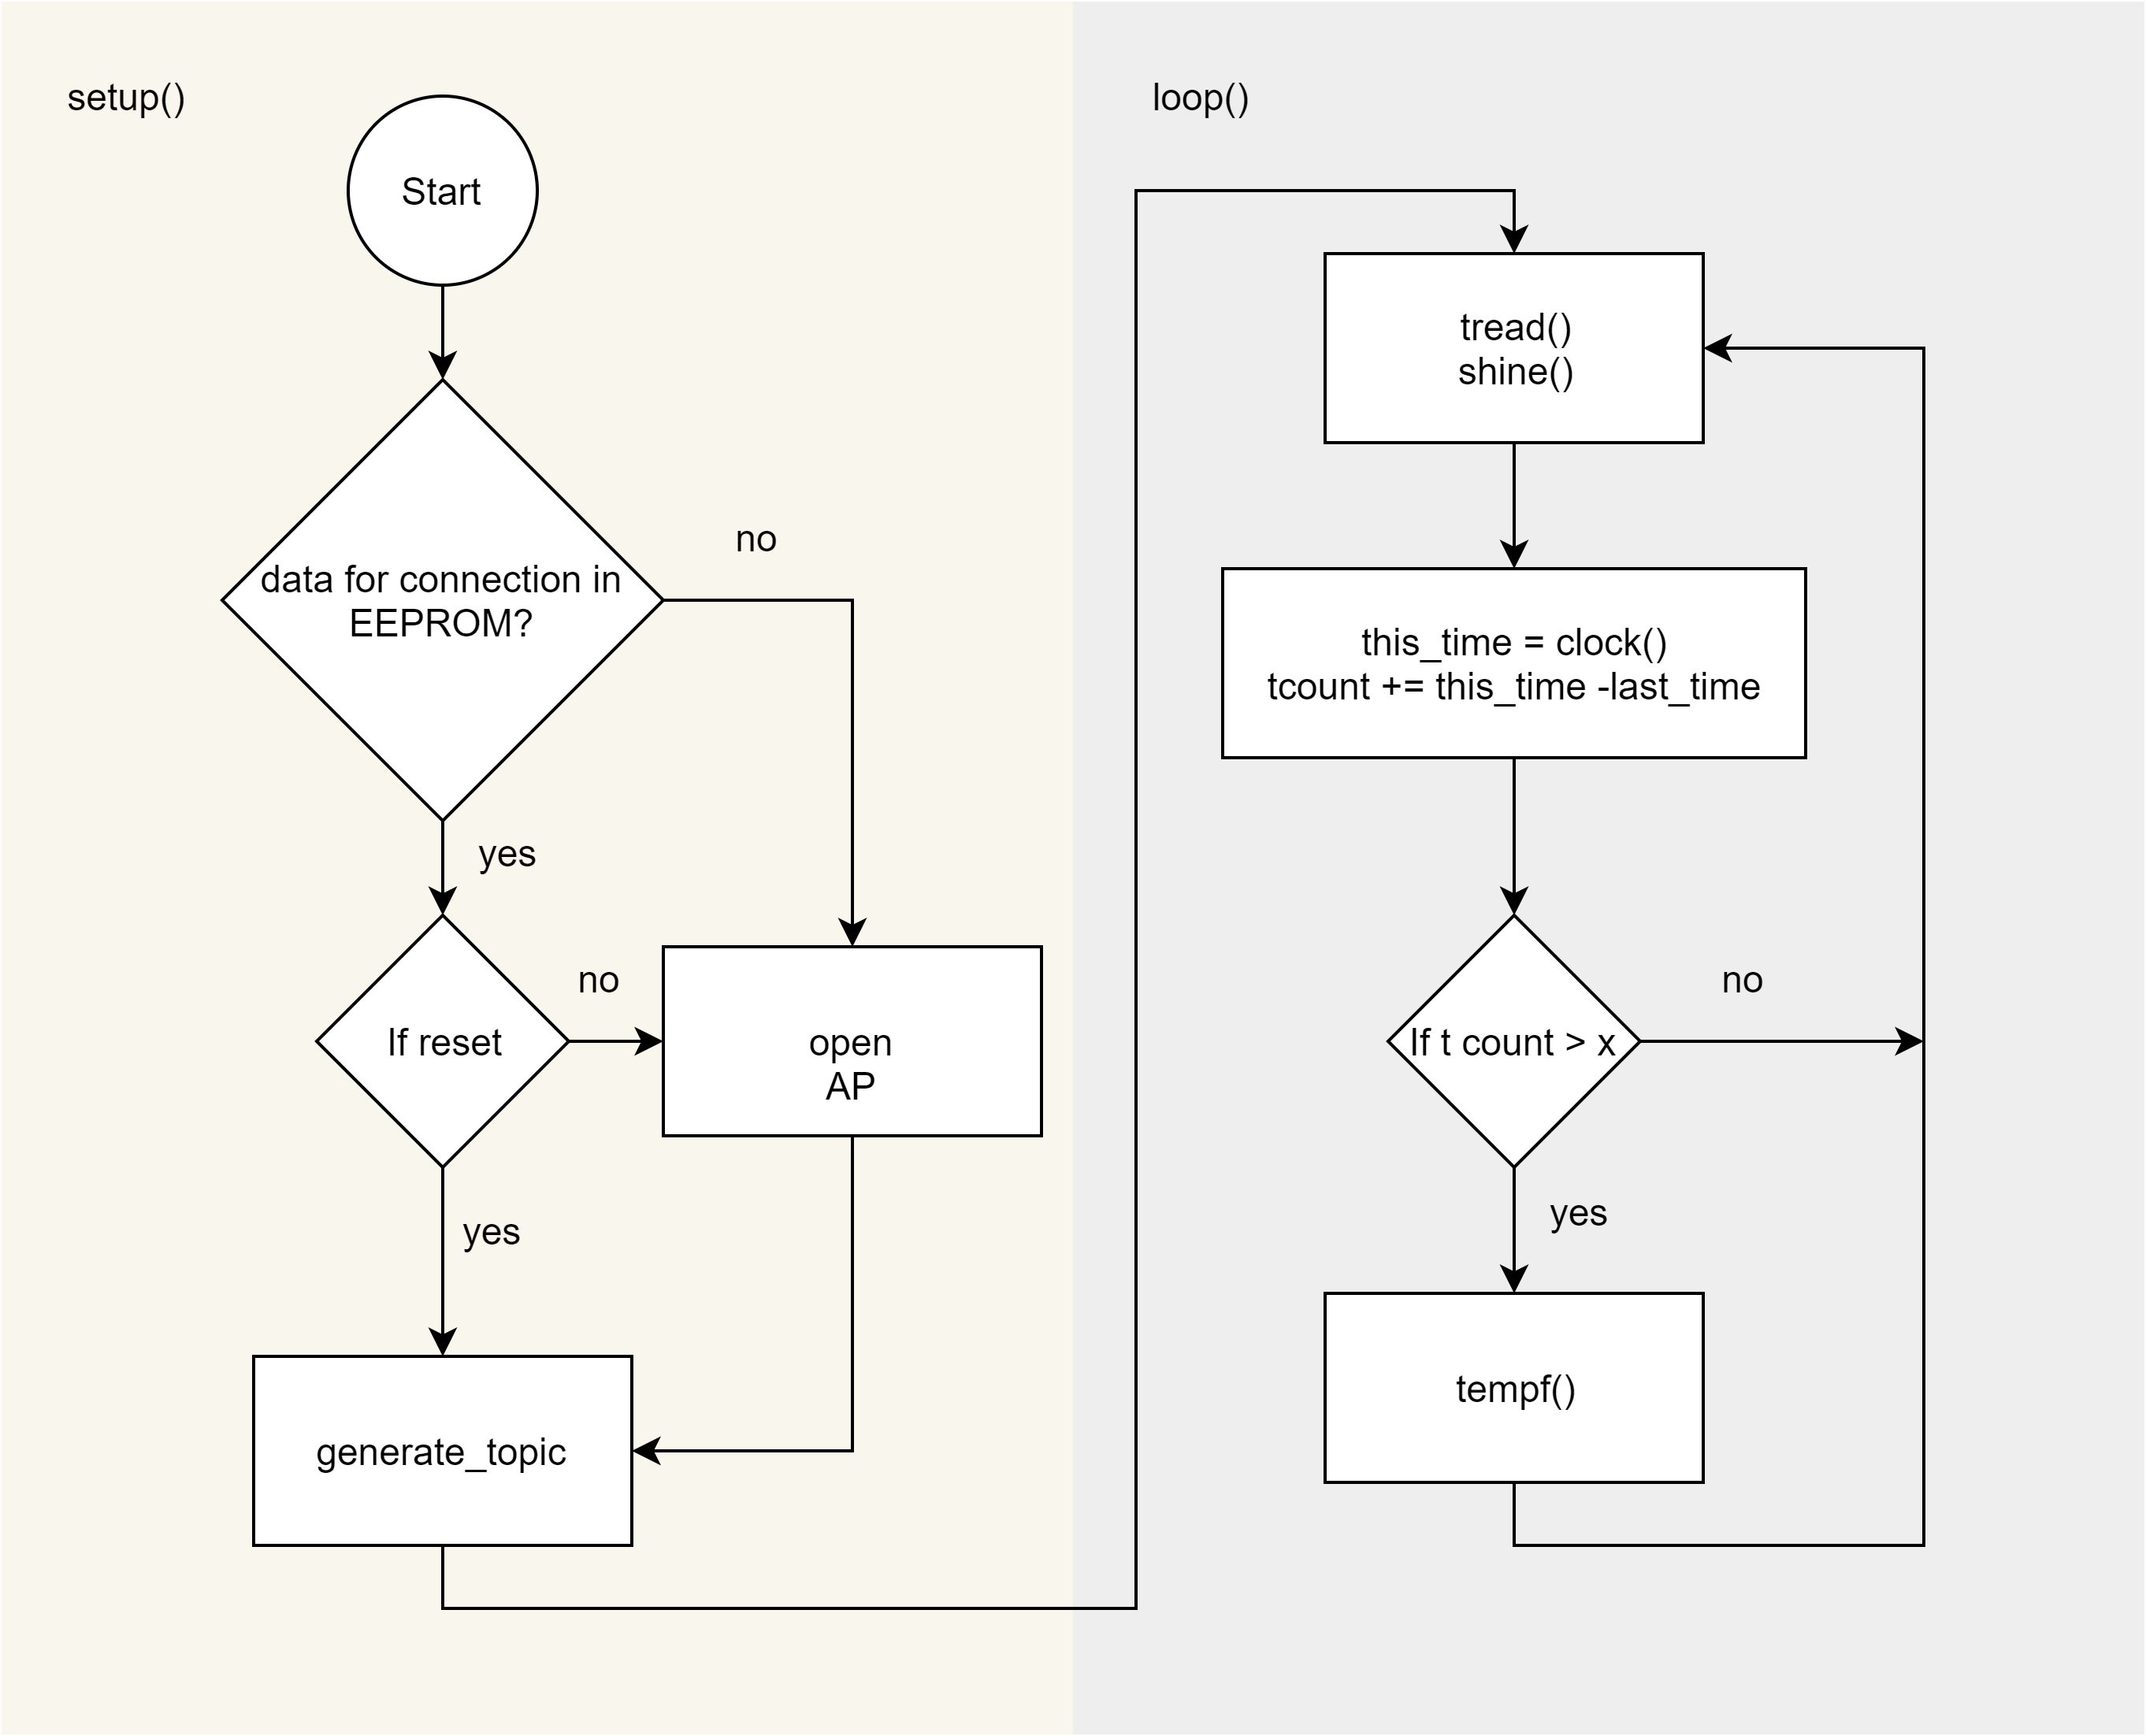
\includegraphics[width=\textwidth]{graphics/StatemaschineSensor.png}
	\caption{In dieser Abbildung ist das Statediagram vom Sensorboard abgebildet}
	\label{pic: statemaschine sensor}
\end{figure} 

\newpage

\subsubsection{setup()}\label{subsubsec: sensor setup}
Wird der Mikrocontroller gestartet so werden als erstes Configurations-Daten im EEPROM gesucht. Werden keine Daten gefunden oder wird die Reset-taste betätigt wird ein Accespoint eröffnet und Confugurations Parameter können mittels Browser eingegeben werden. Dieser Vorgang wird im Kapitel Kommunikation genauer beschrieben. Als nächster Schritt werden für die MQTT-Messages die Topics anhand der Bordbezeichnung und der Anwendung generiert. Die Bordbezeichnung wird im Configportal eingegeben und im EEPROM abgespeichert, sie dient dazu, wenn mehrere Boards installiert werden um die empfangenen Nachrichten zu unterscheiden. Eine mögliche Topic für eine MQTT Nachricht wenn beispielsweise der erste Taster betätigt wird kann folgendermassen aussehen: "data/sesnorboard/wohnzimmer/S1" in diesem Fall wurde die Bordbezeichnung Wohnzimmer gewählt. 

\subsubsection{loop()} \label{subsubsec: sensorloop}
Im loop() wird als erstes die Funktion tread(), dann shine() aufgerufen, danach wird die Momentane Zeit mit der Funktion clock() geholt. In der Variabel count wird die Zeitdifferenz zwischen den wiederholenden Durchgängen von touch() addiert. Dies passiert solange bis der Wert x erreicht ist, in diesem Fall alle 10 Sekunden. Wenn der Wert x erreicht ist wird die Funktion tempf() aufgerufen, mit dieser wird mittels NTC die Temperatur gemessen. Im gleichen Zyklus wie die Temperaturmessungen Durchgeführt werden, wird die Staus LED geschaltet, so kann überprüft werden, ob sich das Bord im normalen Betrieb befindet, sprich der loop() wird gewiss komplett Durchlaufen. Die Funktionen sind in der nachfolgenden Abbildung abgebildet und werden anschliessend erläutert.

\begin{figure}[H]
	\centering
	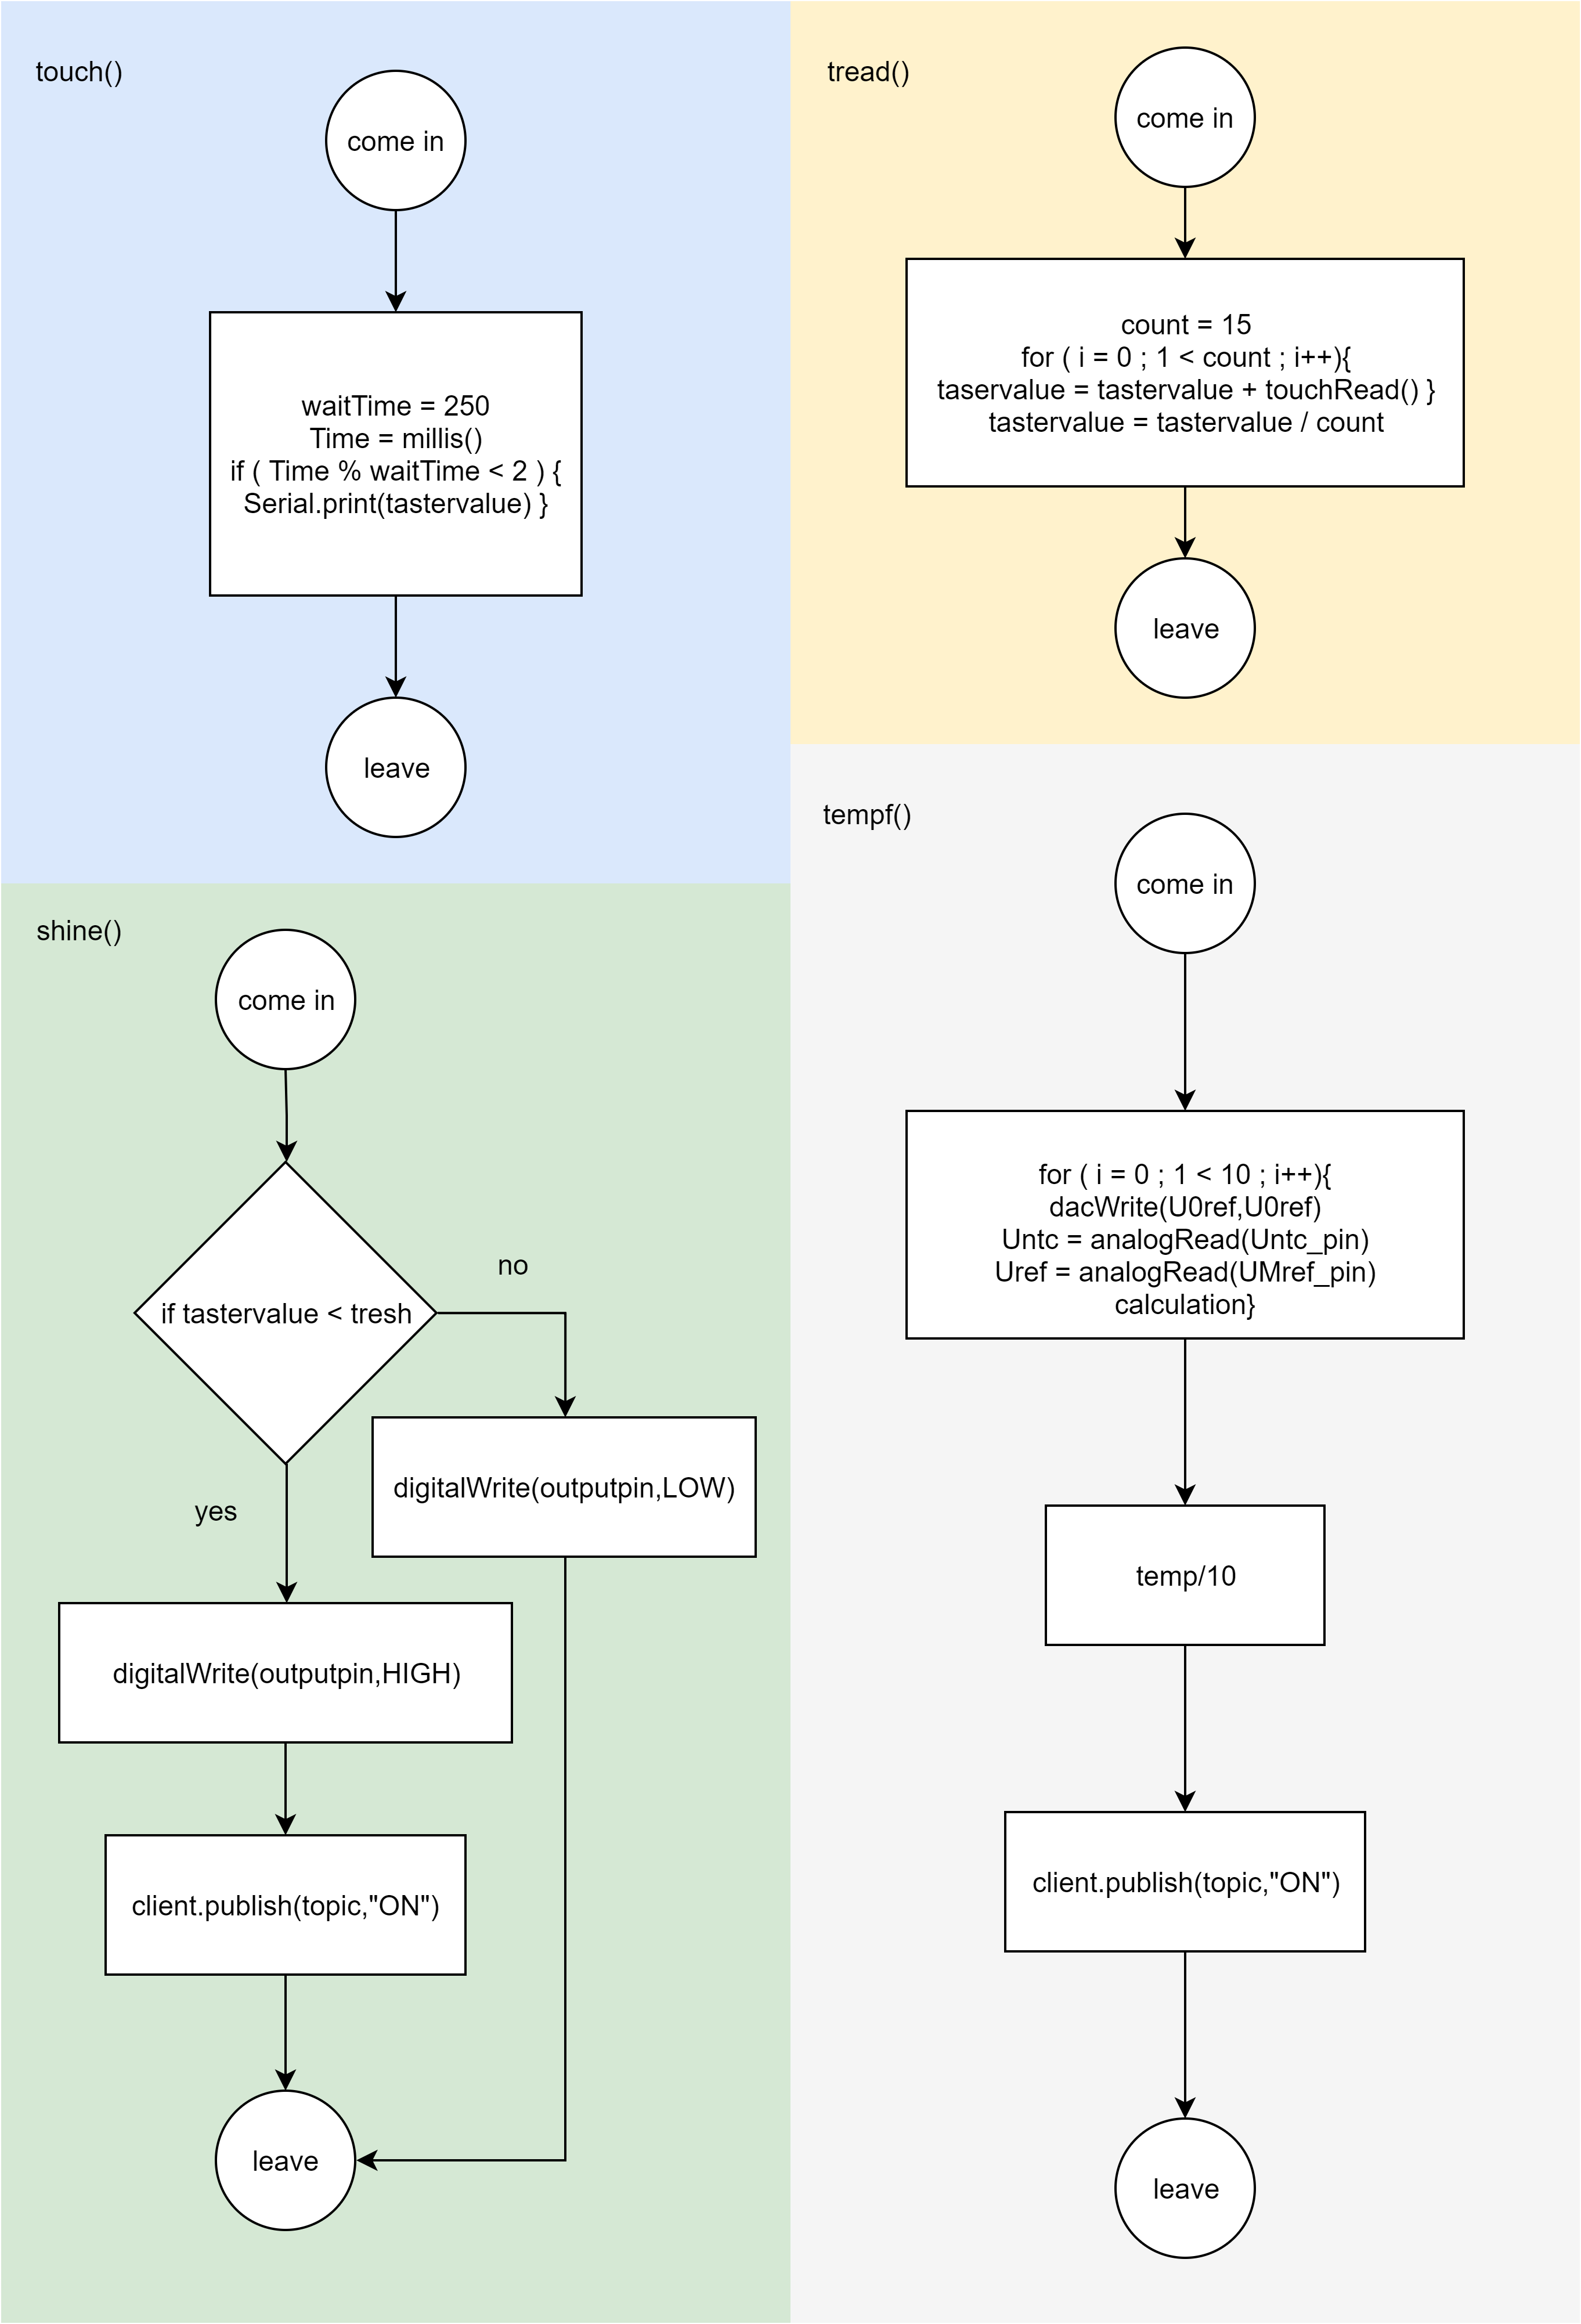
\includegraphics[width=\textwidth]{graphics/FunktionenSensor.png}
	\caption{In dieser Abbildung sind die Funktionen vom Sensorboard abgebildet}
	\label{pic: funktionen sensor}
\end{figure}   
\subsubsection{touch()} 
Wie in der Abbildung \ref{pic: statemaschine sensor} zu erkennen ist, wird die Funktion touch() nicht aufgerufen. Sie dient alleine zum debuggen also um den optimalen tresh Wert zu finden. Dieser Wert definiert ab wann die Touchsensoren als gedrückt erkannt werden. In der Funktion wird die Variabel waitTime initialisiert mit dem wert 250 weiter wird der Wert millis() in die Variable Time gesetzt. In einer for-wihle werden so lange Time modulo waitTime kleiner als 2 sind, sprich die ersten 2 Millisekunden von 250 Millisekunden, mit Serial.println() der aktuell eingelesene Touchwert ausgegeben. Dieser Wert befindet sich im Ruhezustand um 50-80, wenn eine entsprechende Touch-Taste betätigt wird sinkt dieser Wert auf 10-30.  
\subsubsection{shine()}
In der Funktion shine() wird in einer for-while der Eingelesene Wert das sogenannte taservalue der jeweiligen Touchtasten mit dem Tresholdwert, tresh verglichen. Ist das tastervalue kleiner als tresh, wird eine MQTT-Message mit der entsprechenden Topic und der Payloud "ON" published. Ebenso wird die Led der entsprechenden Taste HIGH gesetzt. Trifft der andere Fall zu, wenn das tastervalue grösser als tresh ist wird die entsprechende Led LOW gesetzt.
\subsubsection{tread()}
In der Funktion tread() werden in einer for-while die aktuellen Werte der vier Touch-Tasten eingelesen und in den int-array tastervalue gesetzt, um Ausreisser zu eliminieren, wird ein Mittelwert erstellt. Es werden jeweils 15 Messungen addiert und aschliessend durch die Anzahl Messungen dividiert.  
\subsubsection{tempf()} \label{tempf}
In dieser Funktion wird die Temperatur mit dem NTC ermittelt. So wird als erstes $U_{ref}$ und $U_{ntc}$ als ADC-Wert eingelesen und über 10 Werte gemittelt. Danach wird eine Geradengleichung (Gl.: \ref{eq: U_ADC_sensor}) verwendet, um die ADC-Werte in eine Spannung zu konvertieren. Wie im Kapitel \ref{Temperatursensor} beschrieben und in der Abbildung \ref{pic: Temperatursensor} ersichtlich, bildet ein Vorwiderstand von 100\,K$\Omega$ und der NTC einen Spannungsteiler an dem $U_{ref}$ angelegt wird und am NTC die Spannung $U_{ntc}$ gemessen wird. Aufgrund dessen wird der Widerstand des NTCs $R_T$ mit \ref{eq: R_T} berechnet. Für $U_{ref}$ wird maximal eine Spannung von 2.5\,V verwendet, da der ADC danach nicht mehr linear ansteigt, diese Spannung wird mithilfe eines DACs im Setup() ausgegeben. Die Temperatur in Kelvin ergibt sich dann aus der Gleichung \ref{eq: T}, von dieser Zahl wird danach 273.15 abgezogen, um den Wert in °C zu kriegen. Die angesprochene Gerade (Gl.: \ref{eq: U_ADC_sensor}) ist so ausgelegt, dass sie in dem Spannungsbereich der Temperaturmessung funktioniert. Um sie auszulegen und gleichzeitig die Temperatur zu verifizieren wurde folgendes Verfahren angewendet. Als erstes wurde der Temperaturbereich festgelegt, welcher von -5\,°C bis +45\,°C reicht. Dann wurde mittels eines Klimaschrankes \ref{pic: Klimaschrank} die Temperaturen in 5\,°C $\pm$1°C Schritten festgelegt. Um die Temperatur genauer zu messen wurde ein NiCr-Ni Temperaturfühlers (Messgerät Therm 2250-1) verwendet. Der Sensorbaustein und der Temperaturfühler werden nun verschiedenen Temperaturen ausgesetzt und der Sensorbaustein gibt seine ADC-Werte weiter (Tabelle: \ref{tab: Temp_ADC}). Es wurde festgestellt, dass $U_{ref}$ annäherungsweise über die Temperatur konstant bleibt, hier war der ADC Wert 2768\,$\pm$1. $U_{ref}$ wurde ebenso mittels eines Multimeters gemessen und es ergab sich eine Spannung von U$_{ref}$ = 2.39\,V. Die mit dem NiCr-Ni Temperaturfühler gemessenen Temperaturen wurden mithilfe von Gleichung \ref{eq: R_T,2} und \ref{eq: U_ntc} in Spannungen verrechnet, welche an dem NTC anliegen, falls die Toleranz klein genug sind. Diese theoretischen Spannungen wurden genommen, entgegnen den ADC-Werten gesetzt und einen linearen Fit mit QtiPlot erstellt. Die Gerade (Gl.: \ref{eq: U_ADC_sensor}) kam dabei heraus und sie wurde auf die ADC-Werte der Tabelle \ref{tab: Temp_ADC} angewendet, um dann mithilfe von den Gleichungen \ref{eq: R_T} und \ref{eq: T} die Temperaturen zu berechnen, die der Sensorbaustein schlussendlich anzeigt. Diese berechneten Temperaturen des Sensorbausteins wurden dann den gemessenen Temperaturen des Temperaturfühlers in der Tabelle \ref{tab: Temp_ADC} verglichen, die grösste Abweichung war 0.23\,K bei 39.2\,°C, bei welchen der Sensorbaustein 39.43\,°C anzeigen würde. Der Grund dieses Verfahrens ist, dass $U_{ref}$ leicht unterschiedliche Werte annehmen kann, da der DAC nicht genau ist, vereinfacht gesagt wurde im Bereich von $U_{ref}$ = 2.39\, linearisiert. $U_{ref}$ wird wie $U_{ntc}$ gemessen, was bedeutet dass es keine Rolle spielt ob, $U_{ref}$ = 2.30\,V oder 2.4\,V ist.
\\
\begin{center}	
Berechnungen zur Temperaturmessung:
\begin{align}
	U &= ADC \cdot m_{sensor} + b_{sensor} \label{eq: U_ADC_sensor}\\
	\frac{R_T}{R_V} &= \frac{U_{ntc}}{U_{ref}\;-\;U_{ntc}} \label{eq: R_T}\\
	T &= \frac{1}{\frac{1}{T_N}+\frac{1}{B} \cdot ln(\frac{R_T}{R_0})}\; 
	\widehat{=}\; \frac{1}{\frac{1}{T_N}+\frac{1}{B} \cdot ln(\frac{R_T}{R_V})}  \label{eq: T}\\
	R_T &= R_0 e^{B\left(\frac{1}{T} - \frac{1}{T_0}\right)} \label{eq: R_T,2}\\
	U_{ntc} &= \frac{R_T}{(R_V + R_T)} \cdot U_{ref} \label{eq: U_ntc}
\end{align}
\\
Konstanten zur Temperaturmessung:
\begin{align*}
	m_{sensor} &= 0.0008155002\,V\\
	b_{sensor} &= 0.1369856\,V\\
	R_V &= 100\,k\Omega\; \text{(Vorwiderstand)}\\
	R_0 &= 100\,k\Omega\; \text{(Widerstand des NTCs bei 25\,°C)}\\
	B &= 4250\,K\; \text{(B-Konstante des NTCs)}
\end{align*}
\\Variablen zur Temperaturmessung:
\begin{align*}
 U_{ntc}\; &\text{(Spannung über NTC)}\\
 U_{ref}\; &\text{(Spannung über Vorwiderstand und NTC)}\\
 U\; &\text{(Spannung allgemein)}\\
 ADC\; &\text{(ADC-Wert allgemein)}\\
 T\; &\text{(momentante Temperatur in Kelvin)}\\
\end{align*}
\end{center}

\begin{table}[H]
	\begin{tabular}{|c|c|c|c|}
		\hline
		\textbf{\begin{tabular}[c]{@{}c@{}}Temperatur in °C \\ (Therm 2250-1)\end{tabular}} & \textbf{\begin{tabular}[c]{@{}c@{}}ADC Wert \\ von $U_{ntc}$\end{tabular}} & \textbf{\begin{tabular}[c]{@{}c@{}}Temperatur in °C \\ (Sensorbaustein)\end{tabular}} & \multicolumn{1}{l|}{\textbf{Abweichungen in °C}} \\ \hline
		-4.6 & 2254 & -4.42 & 0.18 \\ \hline
		0.6 & 2119 & 0.65 & 0.05 \\ \hline
		5.6 & 1966 & 5.73 & 0.13 \\ \hline
		10.2 & 1826 & 9.99 & -0.21 \\ \hline
		14 & 1687 & 14.02 & 0.02 \\ \hline
		20.2 & 1474 & 20.02 & -0.18 \\ \hline
		25.1 & 1300 & 24.93 & -0.17 \\ \hline
		29.7 & 1138 & 29.64 & -0.06 \\ \hline
		34.3 & 980 & 34.50 & 0.20 \\ \hline
		39.2 & 832 & 39.43 & 0.23 \\ \hline
		44 & 709 & 43.93 & -0.07 \\ \hline
	\end{tabular}
	\caption{Mit dem Therm 2250-1 aufegenommene Temperaturwerte und die ADC Werte von $U_{ntc}$, welche zu den Temperaturen des Sensorbausteins berechnet wurden, dazu die Abweichungen der Temperaturen voneinander.}
	\label{tab: Temp_ADC}
\end{table}

\begin{figure}[H]
	\centering
	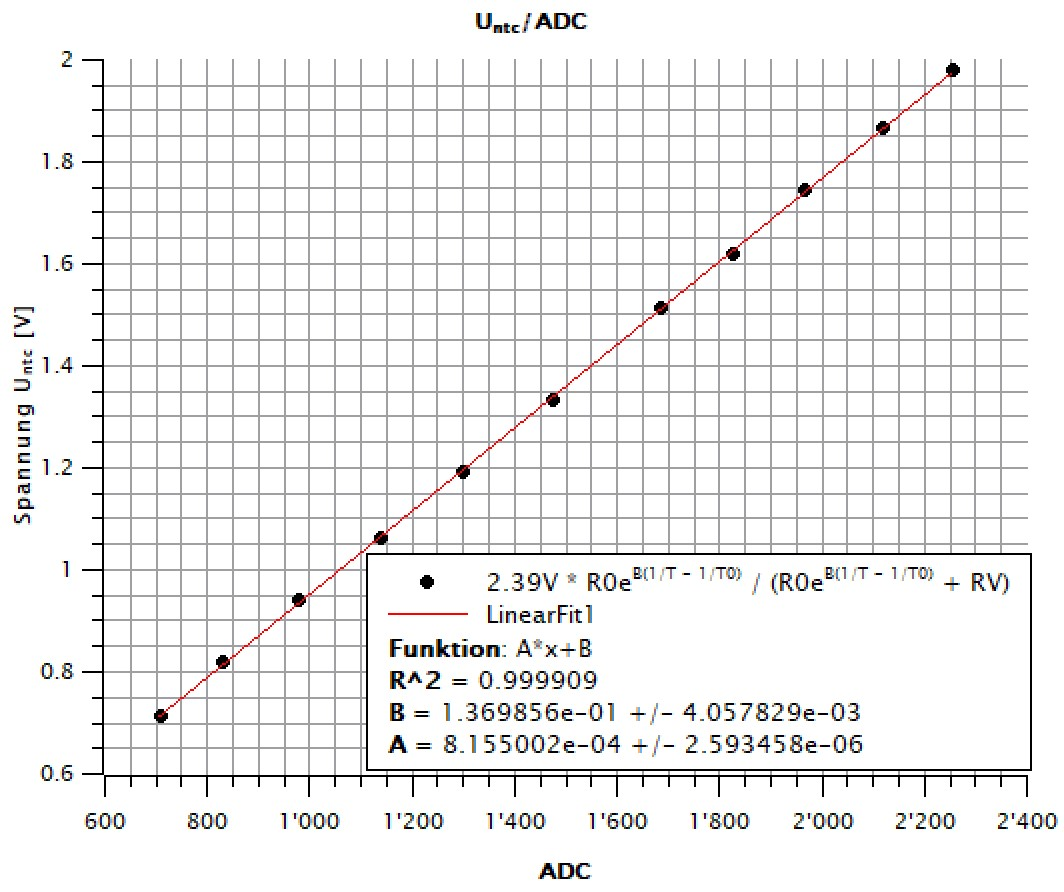
\includegraphics[width=0.9\textwidth]{graphics/Untc_ADC.jpg}
	\caption{$U_{ntc,berechnet}/ADC$}
	\label{pic: Untc_ADC}
\end{figure}

\begin{figure}[H]
	\centering
	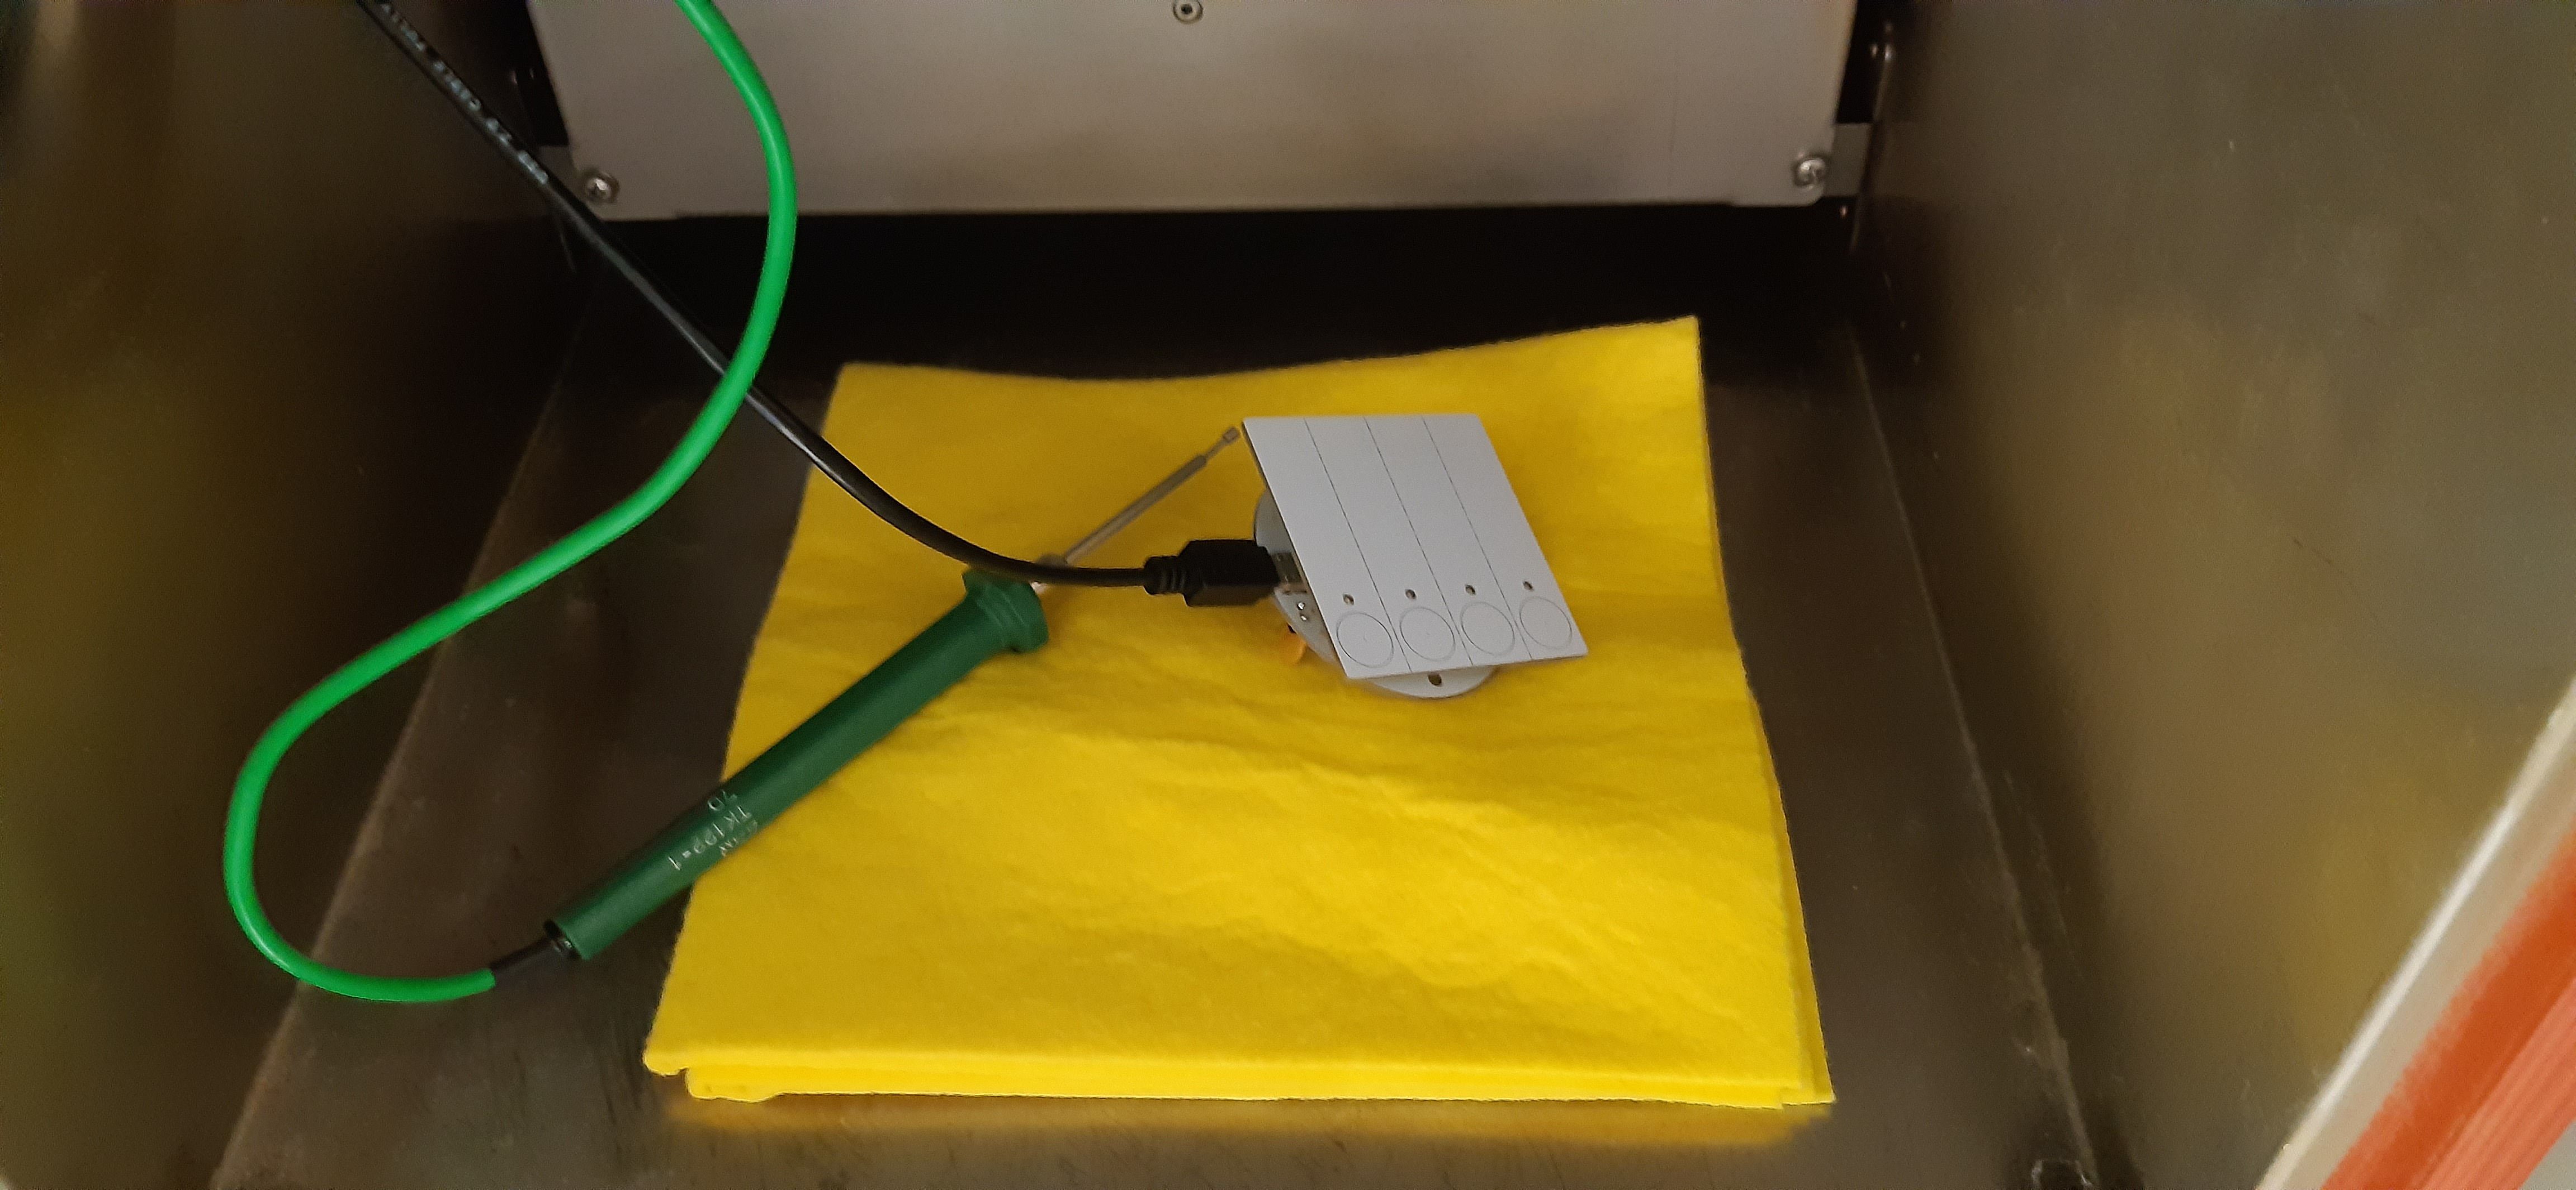
\includegraphics[width=0.90\textwidth]{graphics/Klimaschrank.jpg}
	\caption{Temperaturmessung im Klimaschrank}
	\label{pic: Klimaschrank}
\end{figure}

\newpage
\subsection{Programmcode Aktorbord}
Die Aufgabe des Aktorbord besteht darin, dass Befehle empfangen, verarbeitet und ausgeführt werden. Es befinden sich vier Relais auf dem Bord,welche 230 Volt schalten können, diese werden mit Digitalen IO Pins angesteuert. Eine weitere Aufgabe ist die Ausgabe von zwei DC-Spannnugen 0-10 Volt. Die jeweilige Spannung entsteht durch ein PWM Signal. Eine letzte Aufgabe ist, 0-10 Volt einlesen. Das Eingangssignal gelangt über ein Spannungsteiler an den AD-Wandler. Der Mikrocontroller wertet das Signal aus und generiert eine MQTT-Message welche in einem Periodischen Zyklus publishd wird.    


\subsubsection{	Übersicht} 
\begin{figure}[H]
	\centering
	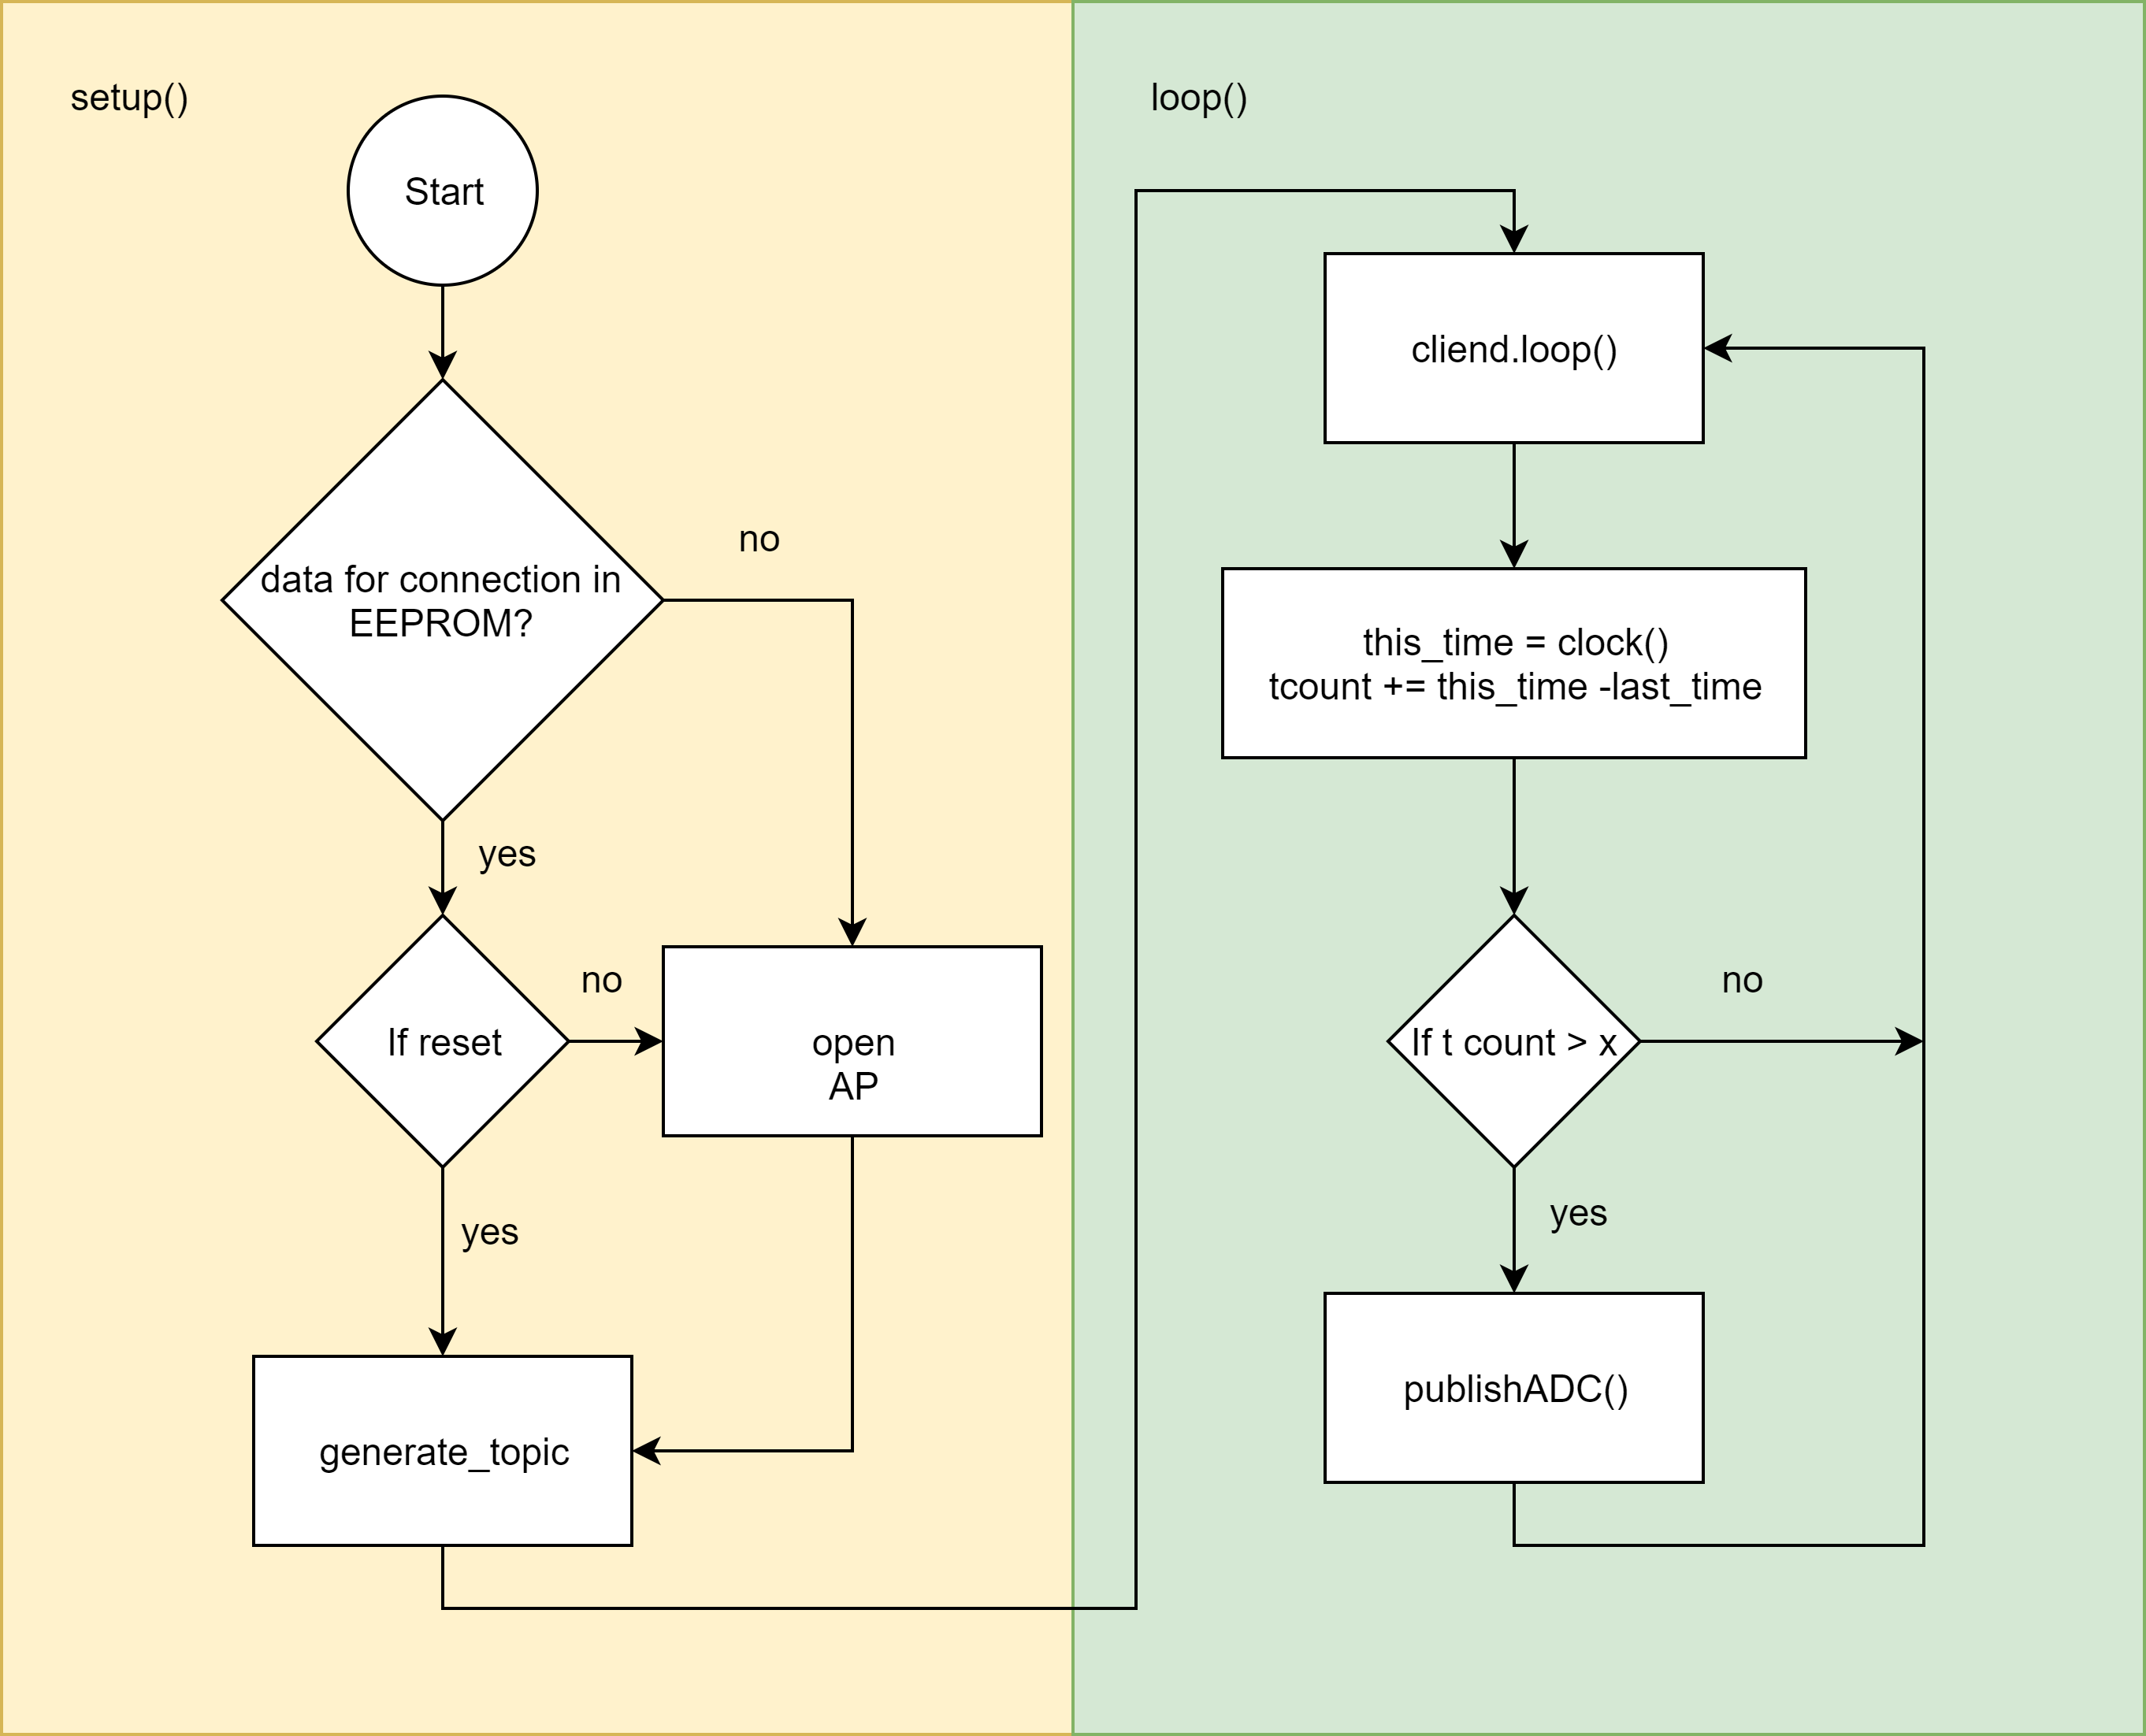
\includegraphics[width=\textwidth]{graphics/StatemaschineAktor.png}
	\caption{In dieser Abbildung ist das Statediagram vom Aktorbord abgebildet}
	\label{pic: statemaschine Aktor}
\end{figure} 
\newpage

\subsubsection{setup()}
In der Abbildung ist zu erkennen, dass genau der gleiche Ablauf wie beim Sensorprint \ref{subsubsec: sensor setup} statt findet. Wird aber der Programm Code selber betrachtet werden andere Bezeichnungen wie andere Definitionen von pinMode() usw. im Bezug zum Sensorbord Festgestellt werden. 
\subsubsection{loop()}
Im loop() wird als erstes die Funktion clien.loop() aufgerufen. Diese Funktion ist im wesentlichen zuständig, dass MQTT Befehle empfangen und verarbeitet werden, Sie wird anschliessend ausführlich erläutert. In einem weiteren Schritt wird wie im loop() vom Sensorbord beschrieben \ref{subsubsec: sensorloop}, Periodischer Zyklus erstellt welche nur alle 10 Sekunden ausgeführt wird. In diesem Zyklus befindet sich die Funktion publishADC, welche die gemessenen Werte von den 0-10 Volt Eingenen als MQTT-Message published.
\begin{figure}[H]
	\centering
	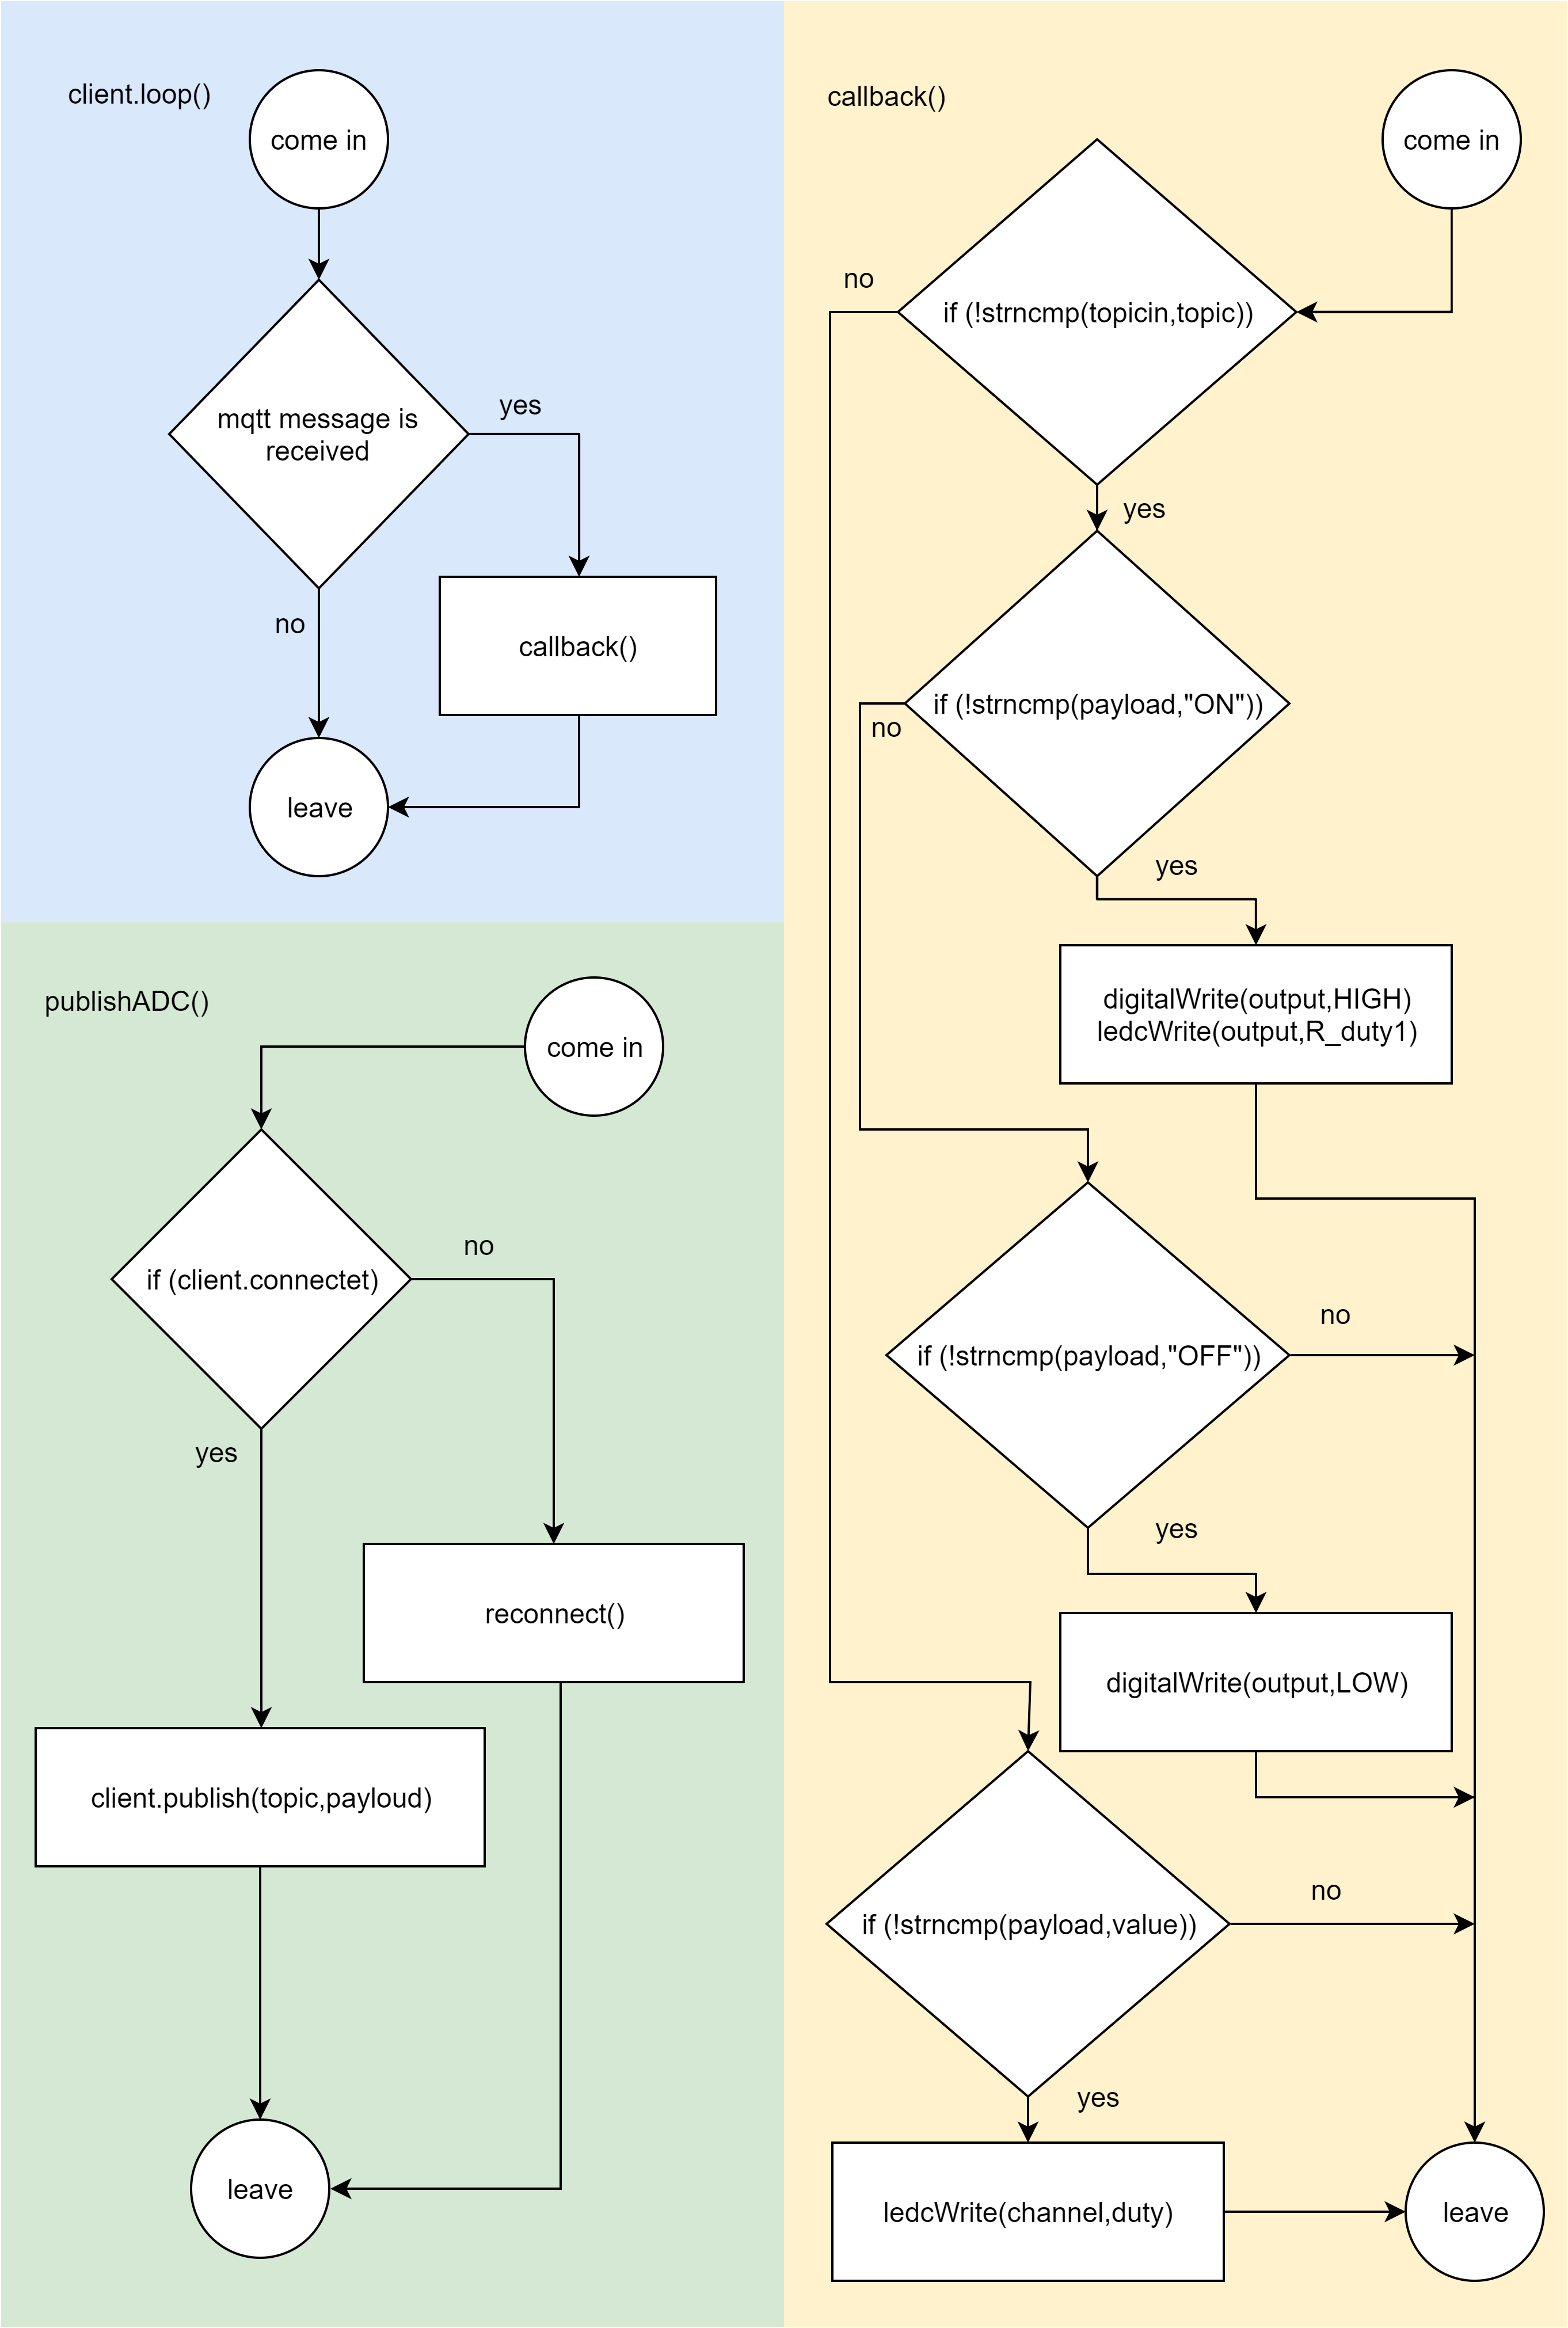
\includegraphics[width=\textwidth]{graphics/FunktionenAktor.png}
	\caption{In dieser Abbildung sind die Funktionen vom Sensorboard abgebildet}
	\label{pic: funktionen Aktor}
\end{figure}   
\subsubsection{client.loop()}
 Das Objekt \textit{client} wurde aus dem PubSubClient gebaut, wo der loop() implementiert wurde. Als erstes wird die Verbindung zum MQTT-Broker überprüft, dann bei bedarf die MQTT-Message empfangen und vorbereitet, dass sie in der Funktion callback()  genutzt werden kann. callback() wird aufgerufen.
 \subsubsection{callback()}
 In dieser Funktion wird als erstes der Inhalt von der Empfangenen Topic überprüft, fällt der Vergleich positiv aus wird der Inhalt der Payload überprüft. Die vier Verschiedenen Relais und die zwei Analogausgänge unterscheiden sich an Hand der Topic. Bei den Relais ist die Payload ON oder OFF und das Relais wie auch das Led des entsprechenden Relais wird in den geforderten zustand gesetzt. Trift die Topic auf ein Analog Ausgang wird nach Umwandlung der Payloud von einem String in ein Float, das PWM-Signal für den entsprechenden Ausgang gesetzt. Den Duty cycle für das PWM Signal wird berechnet indem die gewünschte Spannung voltage folgender Massen verrechnet wird : $(voltage/3.2 \cdot 4095)/3.25$. 3.2 sind es, weil die Verstärkung 3.2 beträgt und 3.25, weil das die Amplitude des PWM Signales ist. Leider kann die Amplitude abweichen und ist nicht sehr genau. Mehr zur Genauigkeit in der Validierung.
 
 \subsubsection{publishADC()}
Mit dieser Funktion werden die 0-10 Volt Eingänge ausgewertet und Resultate als MQTT-Message versendet. Der jeweiligen Messreihe am ADC wird der Mittelwert berechnet, welcher dann von einem float in ein char-Array umgewandelt wird. Als nächstes wird der char-Array und die entsprechende Topic vom PupsubClient veröffentlicht.

\subsection{Task2code()}
Diese Funktion wird im Gegensatz zum Rest des Programms im zweiten Kernel des ESP32 verwendet. Falls ein Relais in der Callback() Funktion gesetzt wird, wird in dieser Funktion die Zeit gemessen und nach 25\,ms wird der Sparmodus für das jeweilige Relais gesetzt. Das setzten des Sparmodus passiert für alle Relais einzeln, es spielt keine Rolle wann ein Relais gesetzt wird, es dauert immer 25\,ms $\pm 3 \,ms$. Der zweite Kernel ist somit nur damit beschäftigt, zu prüfen ob ein Relais aktiviert wurde und es dann nach einer vordefinierten Zeit in den Sparmodus zu bringen.
\newpage

\subsection{Programmcode Openhab}        
Der Aufbau des Systems besteht aus verschiedenen Komponenten welche in nachfolgender Tabelle aufgelistet sind
\begin{table}[H]
	\begin{tabular}{|l|l|}
		\hline 
		Bezeichnung	& Beschreibung \\ 
		\hline 
		Bindings	& Schnittstellen verknüpft verschiedene Dienste miteinander  \\ 
		\hline 
		Things	& Definition von Gerät, Verbraucher, Teilnehmer des Systems  \\ 
		\hline 
		Channel	& Verbindung zwischen Thing und Item  \\ 
		\hline 
		Item	& Repräsentiert Informationen des Gerätes, Schalter, Label usw. \\ 
		\hline 
		Rules	& Festgelegte Regeln für automatische Abläufe\\ 
		\hline 
		Sitmaps	& Benutzeroberfläche, präsentiert Informationen  \\ 
		\hline 
	\end{tabular} 
	\caption{Komponenten Openhab Software \cite{noauthor_introduction_nodate-1}}
	\label{tab: Komponenten Openhab Software}
\end{table}
\begin{figure}[H]
	\centering
	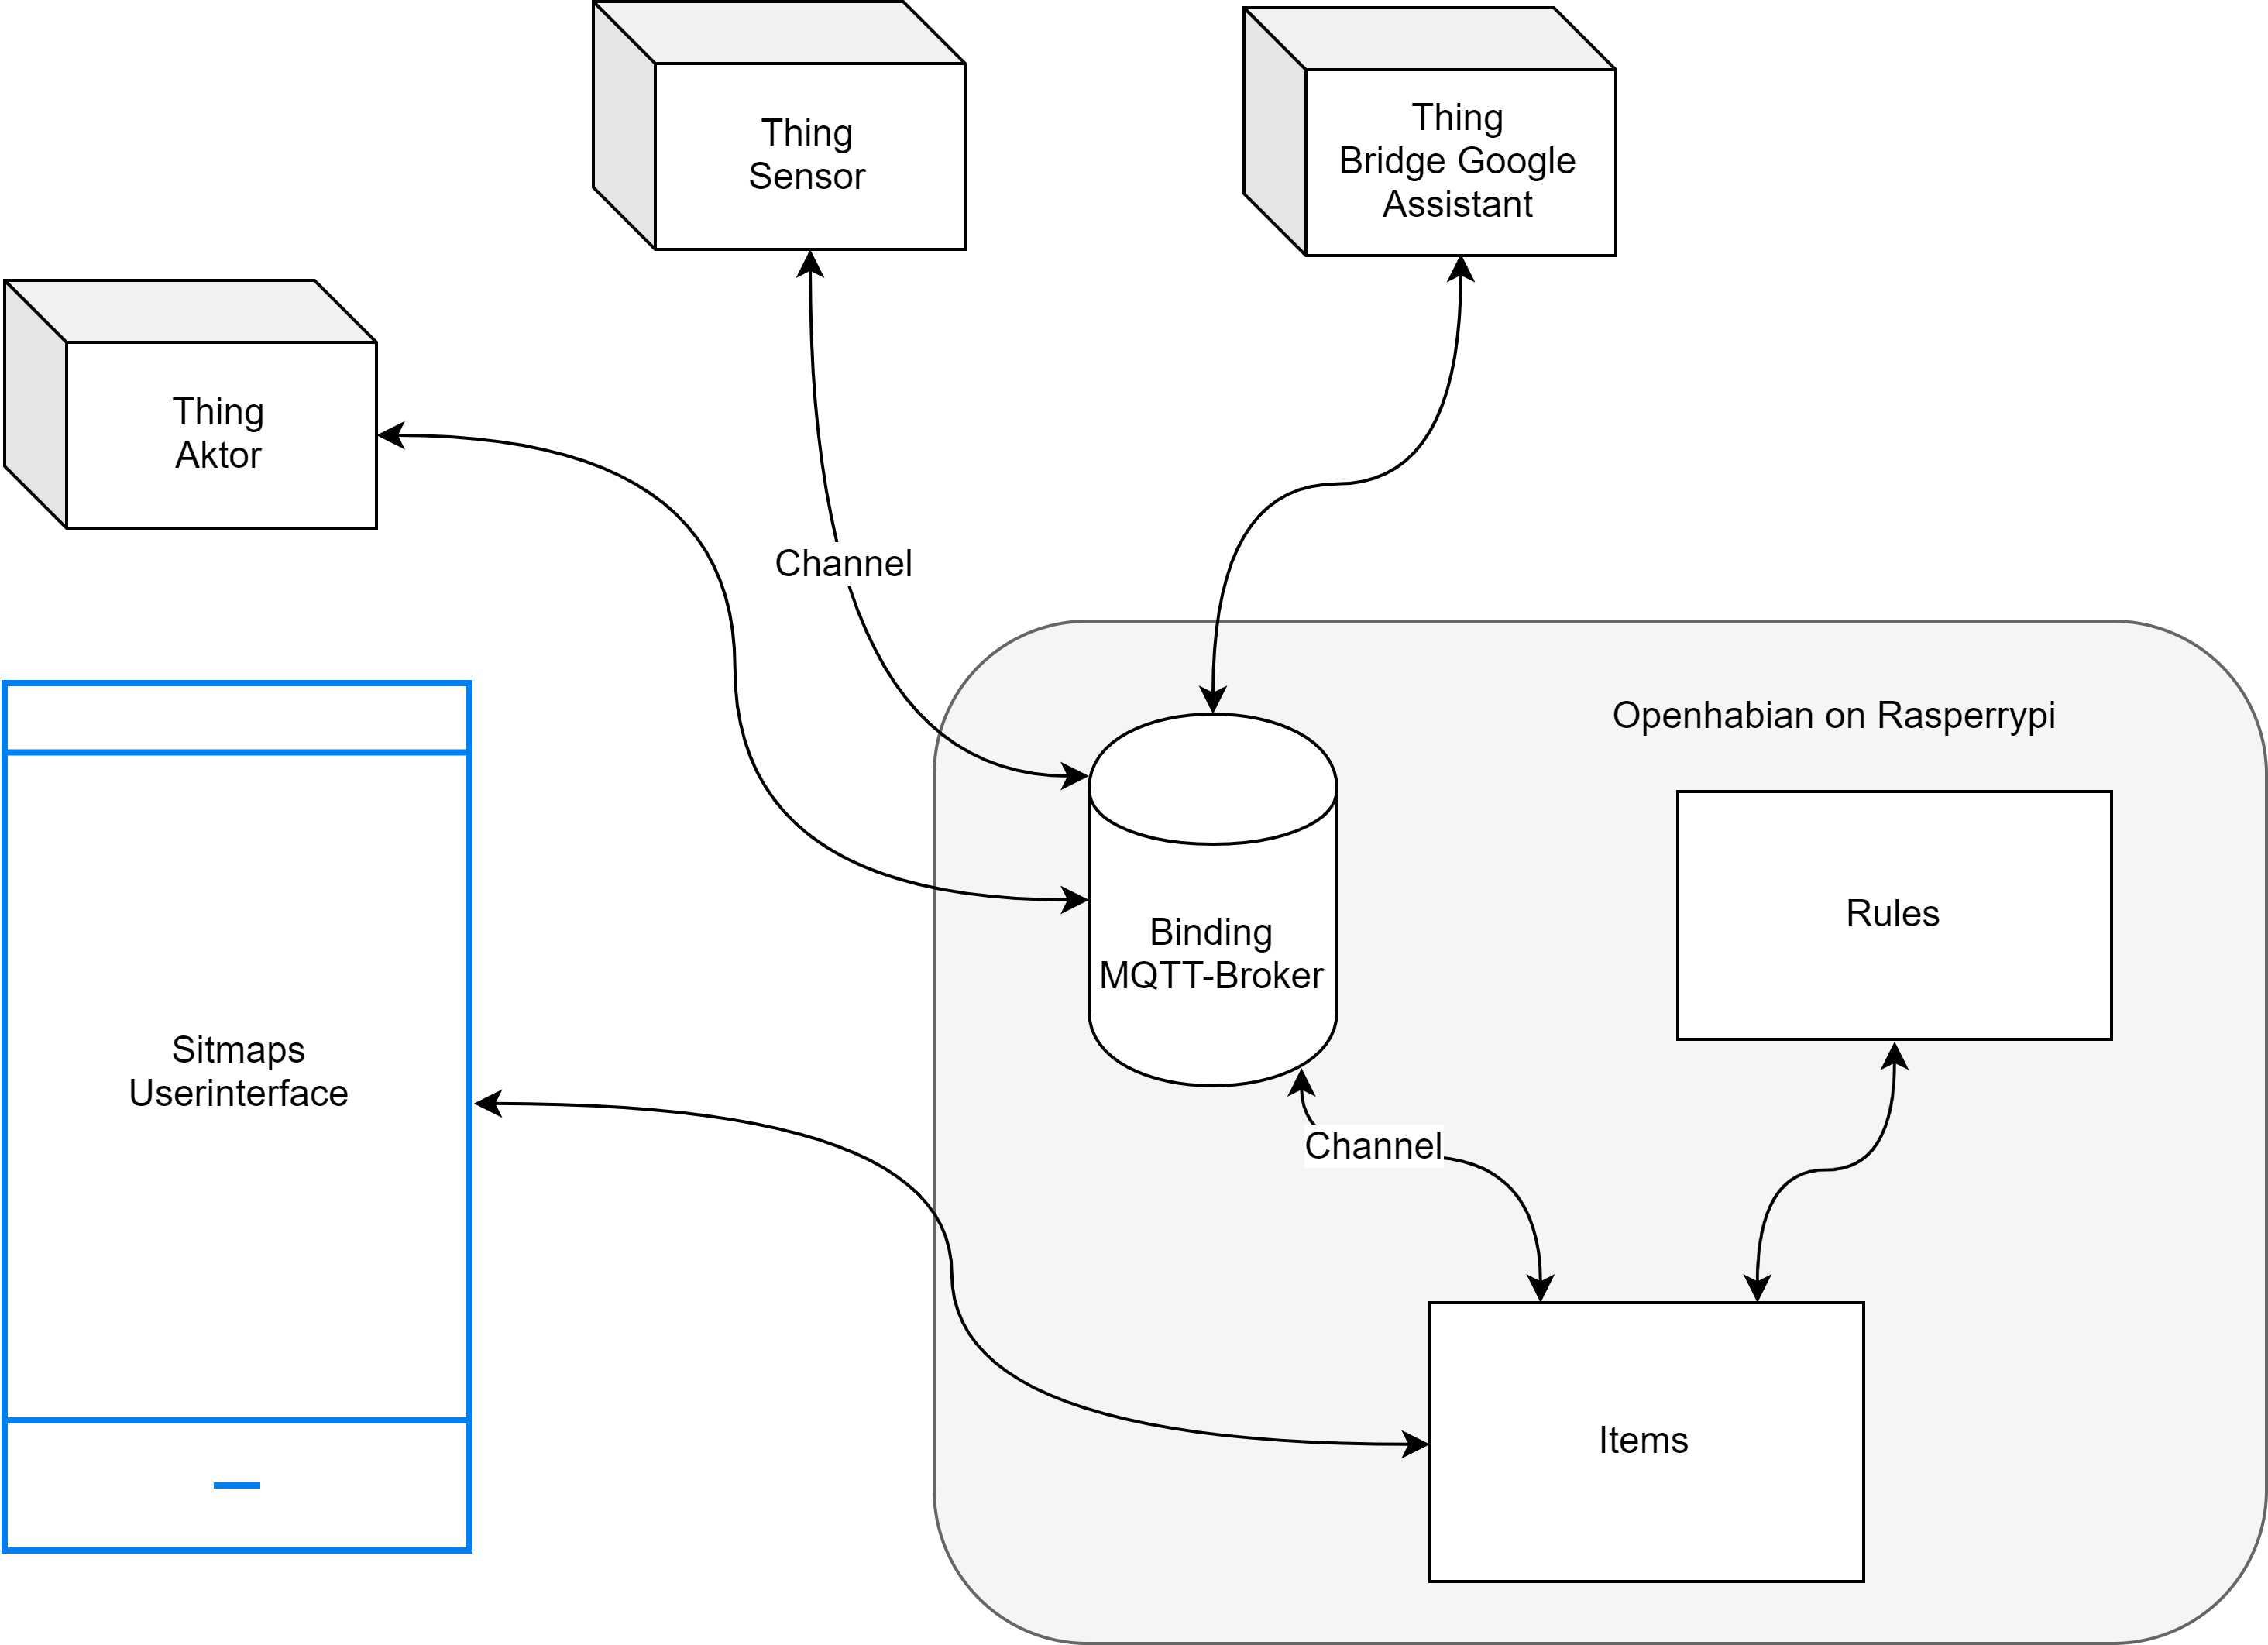
\includegraphics[width=\textwidth]{graphics/Openhabian.png}
	\caption{Komponenten und Verbindungen von Openhab}
	\label{pic: Komponenten Openhab}
\end{figure}   

\subsubsection{Bindings}
Als Schnittstelle von den Items zu den Things wird ein MQTT-Broker benötigt. Um die Systemzuverlässigkeit zu steigern wurde ein eigener Broker Installiert, so kann die Kommunikation auch ohne Netzwerkanschluss ans Öffentliche Netz funktionieren. Ein weiterer Vorteil ist die Sicherheit, es kann auf Passwörter verzichtet werden, da kein Zugriff von ausserhalb des Home-Netzwerk möglich ist.

\subsubsection{Things}
 Als Geräte wurden drei Komponenten hinzugefügt, welche in der Abbildung \ref{pic: Komponenten Openhab} zu erkennen sind. Zum Aktor Thing gelangen im ganzen 8 Channels, um die Relais einzeln anzusprechen wurde pro Relais eine MQTT-Topic erstellt welche je einen Channel verfügt und so mit je einem Item verbunden. Zwei Channel sind für die 0-10 Volt Eingänge und zwei weiter Channel für die 0-10 Volt Ausgänge. Das Sensor Thing verfügt 5 Channel jeder Taster einzeln und ein Channel für die Temperaturmessung.

\subsubsection{Channel}
Die Channes sind die Verbindungen von den Geräten zu den Items also den Software-Zustände, in diesem Projekt werden alle möglichen Fähigkeiten der Geräte genutzt und mit einem Channel gebunden.

\subsubsection{Item}
Das Item zeigt den Status des Verbrauchers oder den gemessenen Wert eines Sensors an. Items werden verwendet wenn Regeln definiert werden,ebenso sind sie mit den Channels verlinkt und können einzeln oder als Gruppen auf dem Sitmap genutzt werden. Als anwendung eines Icons können verschiedene Typen gewählt werden. In diesm Projekt wird in erste Linie der normale Switch verweden welcher in den Zustand ON oder OFF geschalten wird. Für die 0-10 Volt ausgänge werden Dimmer verwendet die als Slider in der Sitmap angezeigt wird und Sie generieren je nach Position einen Wert zwischen 0-1. Um die Messwerte an den 0-10 Volt Eingängen zu verwenden werden die Items als Number genutzt.

\subsubsection{Rules} 
Automatische Prozesse werden mit i Rules definiert. Um das System Benutzerfreundlicher zu Gestalten werden in den Rules die Befehle der Taster verarbeitet und die Entsprechenden Befehle an die Relais generiert. So kann gewährleistet werden, dass der Kunde selber keine Änderungen an den Aktoren und Sensoren selber vornehmen muss. Die Rule Syntax basiert auf Xbase \cite{noauthor_xtext_nodate}. Um die Aufgeben der Befehls Weiterleitung zu übernehmen bestehen die Ruls im wesentlichen aus when und then. In diesem Fall sind sie im Teil when, auf den Empfang des jeweiligen Update getriggert. Somit wird mit einem Update des Status der Teil then ausgelöst, wo sich eine if Bedingung befinden. In diese Bedingung wird der Stus überprüft      

\subsubsection{Sitemaps} 
Als Sitemaps wird das Userinterface bezeichnet. Auf einer Sitemap  gibt es die Möglichkeit verschiedene Elemente in Form von Frame, Text oder Schalter darzustellen, diese Elemente präsentieren Status und Informationen vom System. Das Frame ist Beispielsweise die Aufteilung von einem Haus in seine einzelnen Stockwerke. In den einzelnen Stockwerken werden dann Schalter für jeweilige Geräte als Item hinzugefügt. Mehrere Schalter können als Gruppe zusammen gefasst werden, so kann in zentral Schalter ein/aus realisiert werden. Das erstellte Sitmap ist im Webbrowser mittels IP-Adresse des Servers oder mit dem Openhab Mobile-App erreichbar.


\subsection{Server}\label{subsec: Server}
Als Server für die Openhab Software wird ein Raspberrypi der 4. Generation mit 2 GB RAM eingesetzt, die Installation und Inbetriebnahme wird im Benutzerhandbuch beschrieben. In Openhab wird ebenfalls ein eigener MQTT-Broker eingebunden. Damit diese Broker von jedem Gerät im Lokalen Netzwerk erreicht werden kann, wird dem Server eine Statische IP Adresse vergeben.\\
\\
Um den Sprachassistent einzubinden ist ein weiterer Server mit der Home Assistant Software in das System Integriert worden. Dieser Server wurde auf ein Rasperrypi 4. Generation 2 GB RAM installiert. Der Grund warum nicht beide Server auf dem selben Raspberrypi installiert wurden, ist einerseits, das System ist physikalisch Modular aufgebaut der Sprach Assistent Teil kann als separates Thing (Gerät) betrachtet werden. Andererseits, wenn sich beide Server auf dem Selben Gerät befinden wäre die MQTT-Kommunikation sinnlos.  



\begin{figure}[H]
	\centering
	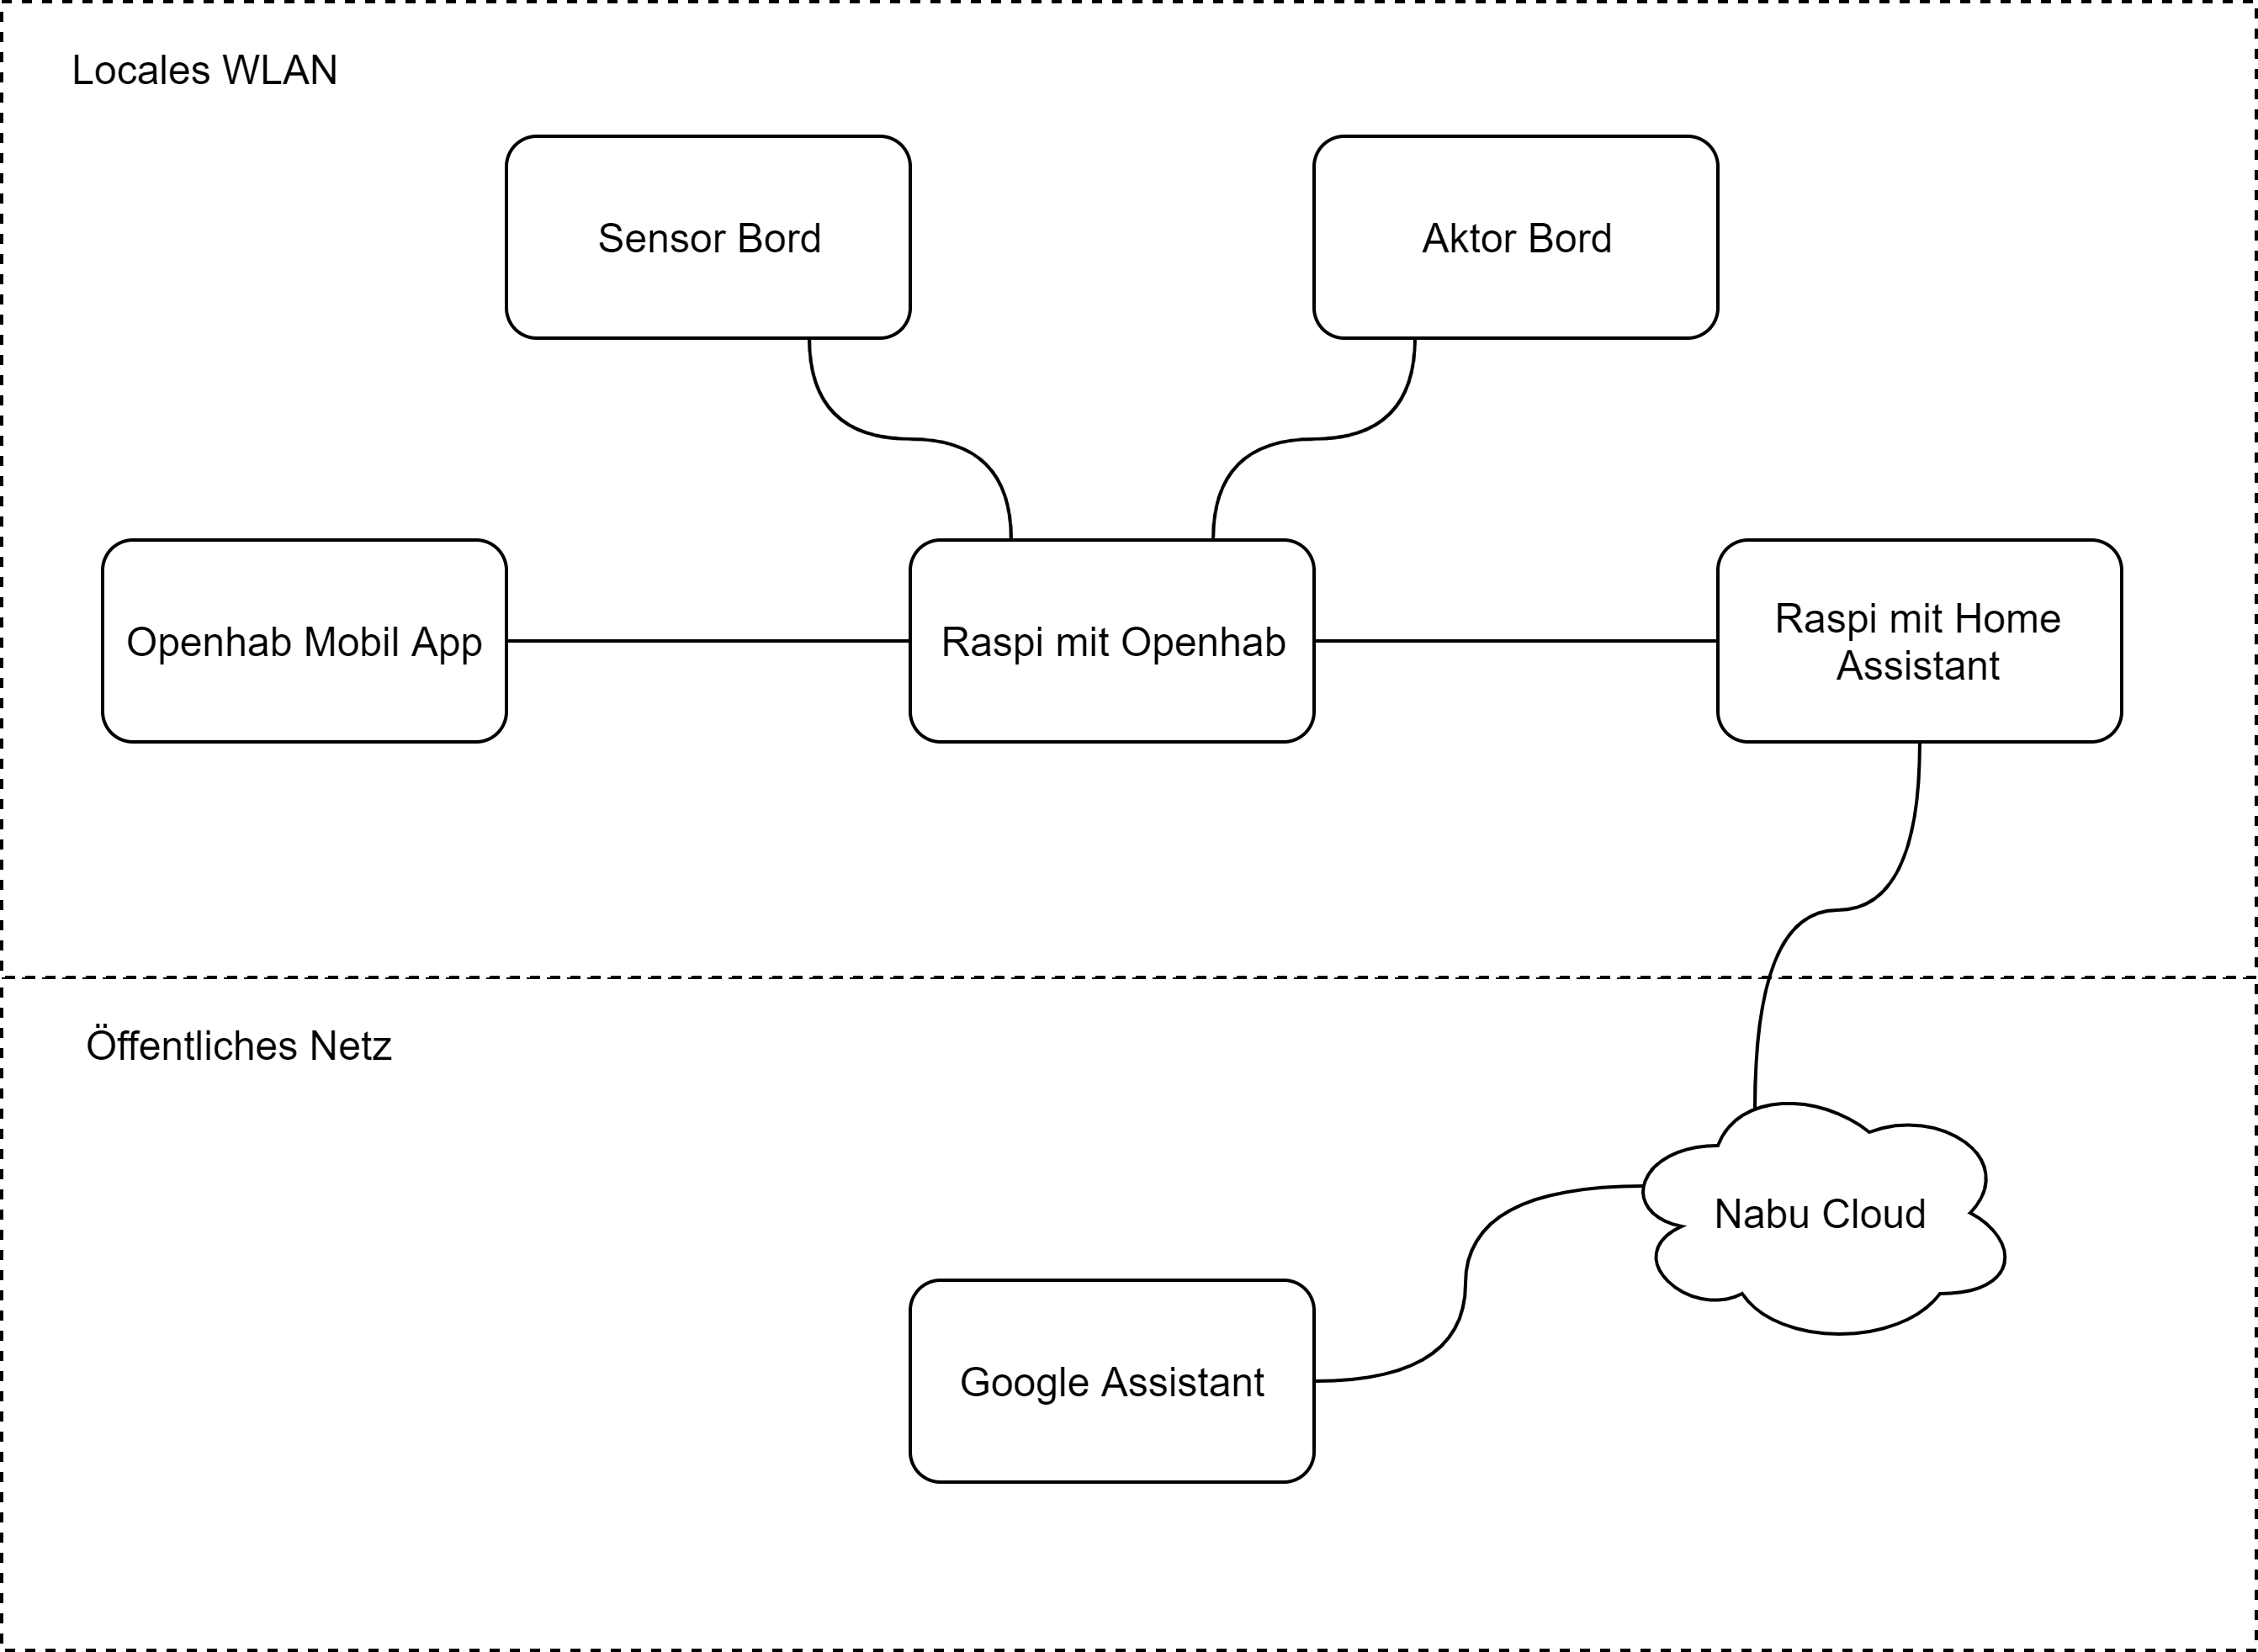
\includegraphics[width=\textwidth]{graphics/Systemubersicht.png}
	\caption{Systemübersicht}
	\label{pic: Systemübersicht}
\end{figure}   

In der Abbildung \ref{pic: Systemübersicht} kann erkannt werden, dass sich beide Server im selben Lokalen Netzwerk befinden. Die Kommunikation zwischen den beiden Server findet über MQTT statt, es besteht die Möglichkeit den Openhab-Server zu umgehen und eine direkte Kommunikation vom Home Assistant zu dem Sensor- oder zum Aktorbord zu realisieren. In diesem Fall müssen aber die Regeln bei welchem Aktion, welche Schalthandlung ausgelösst wird, in den entsprechenden Mikrocontroller Programmiert werden.

\subsection{Sprachassistent}
Der Home Assistant wird als Brücke für den Google Assistant installiert. Mit der Home Assistant Cloud wird eine Verbindung zum Google Assistant hergestellt. Der Grund warum die Verbindung so aufgebaut wird liegt daran, dass dynamische DNS Adresse, SSL-Zertifikate und das öffnen von Ports auf dem Router so umgangen werden. Leider ist die Cloud nach einer Testphase kostenpflichtig. Wird die Lösung ohne Cloud bevorzugt kann nach Anleitung \cite{assistant_google_nodate} gearbeitet werden. Die Cloud ist im /config/configuration.yaml file schon vorinstalliert. Im Webinterface vom Home Assistant kann in den Einstellungen ein Benutzerkonto angelegt werden und schon ist die Cloud aktiv. Das hinzufügen von Schalter um Mqtt-Befehle zu generieren wird im Benutzerhandbuch im Anhang beschrieben. Die Installation auf dem Google Nest, mit einem Smartphone durchgeführt. Mittels Google Home App kann das Gerät 'Home Assistant' hinzugefügt werden.
\begin{figure}[H]
	\centering
	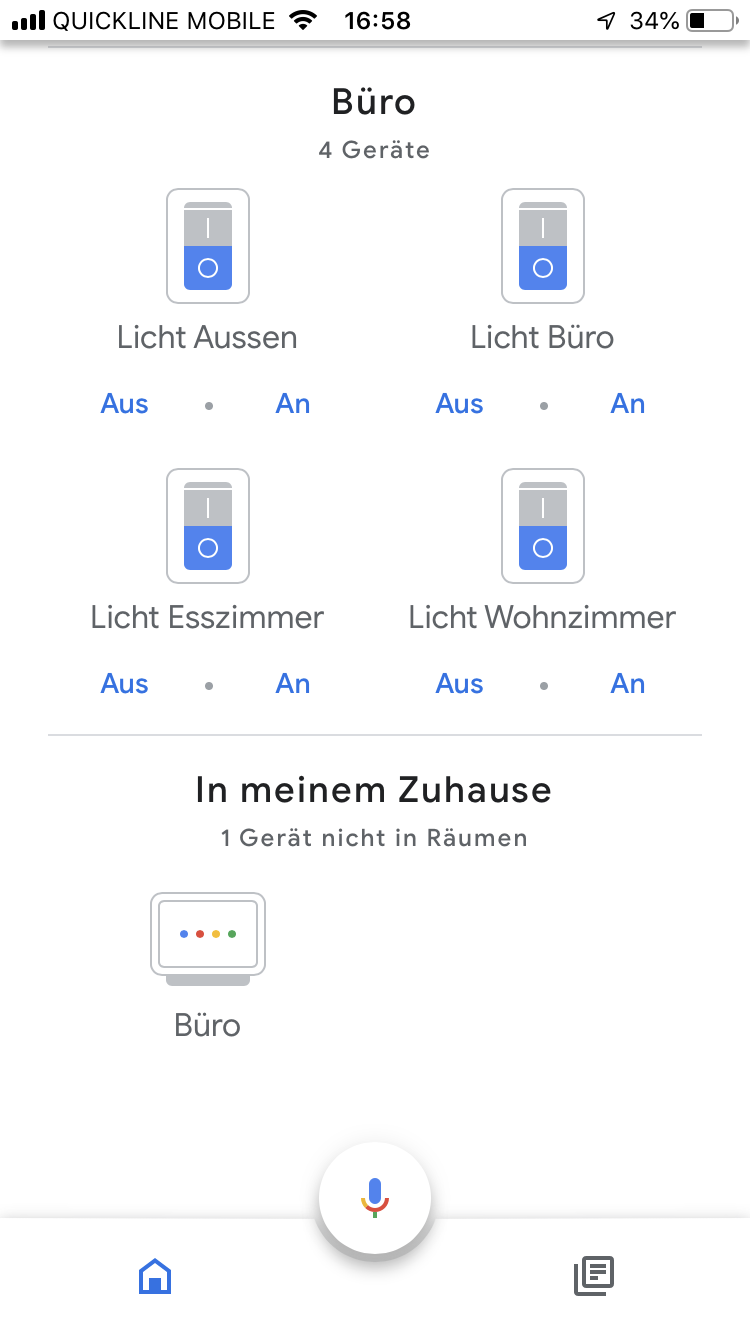
\includegraphics[width=0.5\textwidth]{graphics/GoogleAssistant.png}
	\caption{Google Assistant Mobile-App}
	\label{pic: GoogleAssistant}
\end{figure}   
In der Abbildung \ref{pic: GoogleAssistant} können die Schalter, welche Home Assistant definiert wurden erkannt werden. Sie können mit Sprachbefehl geschalten werden in dem die Schalter Bezeichnung und Zustand genannt wird wie Beispielsweise "Licht Büro ein". Die Verschiedenen Geräte können nebst dem Sprachbefehl in dieser Ansicht mit einem Touch Befehl geschalten werden.





\section{Hardware}
 
\subsection{Sensorbaustein}\label{subsec: Sensorbaustein}
\label{sec: Sensorbaustein}
In diesem Unterkapitel werden die Anforderungen und die Hardware des Sensorbausteins behandelt.
Vom Auftraggeber ist ein Sensorbaustein mit 4-Tasten-Feld und Temperaturfühler gefordert. Der Sensorbaustein wird dabei ähnlich einer Unterputzsteckdose montiert und hat eine WLAN-Schnittelle um die Sensordaten auszulesen. In der Abbildung \ref{pic: Uebersicht_Sensorbaustein} ist die Übersicht des Sensorbausteins dargestellt. Der Baustein wird über einAC/DC Wandler der an der Hauselektrik angeschlossen werden kann mit 5V Spannung versorgt. Da der Mikrocontroller auf 3.3V läuft, wird mithilfe eines weiteren Spannungswandlers die 5 V zu 3.3 V gewandelt, so kann auch der USB Anschluss als Spannungsversorgung dienen. Um den Mikrocontroller zu programmieren steht eine USB zu UART Verbindung, Taster zum Debbuggen, Reseten oder Programmieren und eine Zustands-LED zur Verfügung. Um die Temperatur zu erfassen wird ein NTC verwendet. Da die mitgelieferte Meander-Antenne des ESP32 nur eine kleine Abstrahlleistung hat, kann optional noch eine grössere Antenne, wie z.B. eine zertifizierte grössere Patch-Antenne über RP-SMA angeschlossen werden, falls der ESP32S ausgewählt wird. Der Anwender wird ein Touch-Tastenfeld, sowie dazugehörige LEDs, für die Interaktion mit dem Baustein zur Verfügung haben. Zusammenfassend besteht der Sensorbaustein im wesentlichen aus 3 Teilen, nämlich der Spannungsversorgung, der Hauptplatine und der Frontplatte.

\begin{figure}[H]
	\centering
	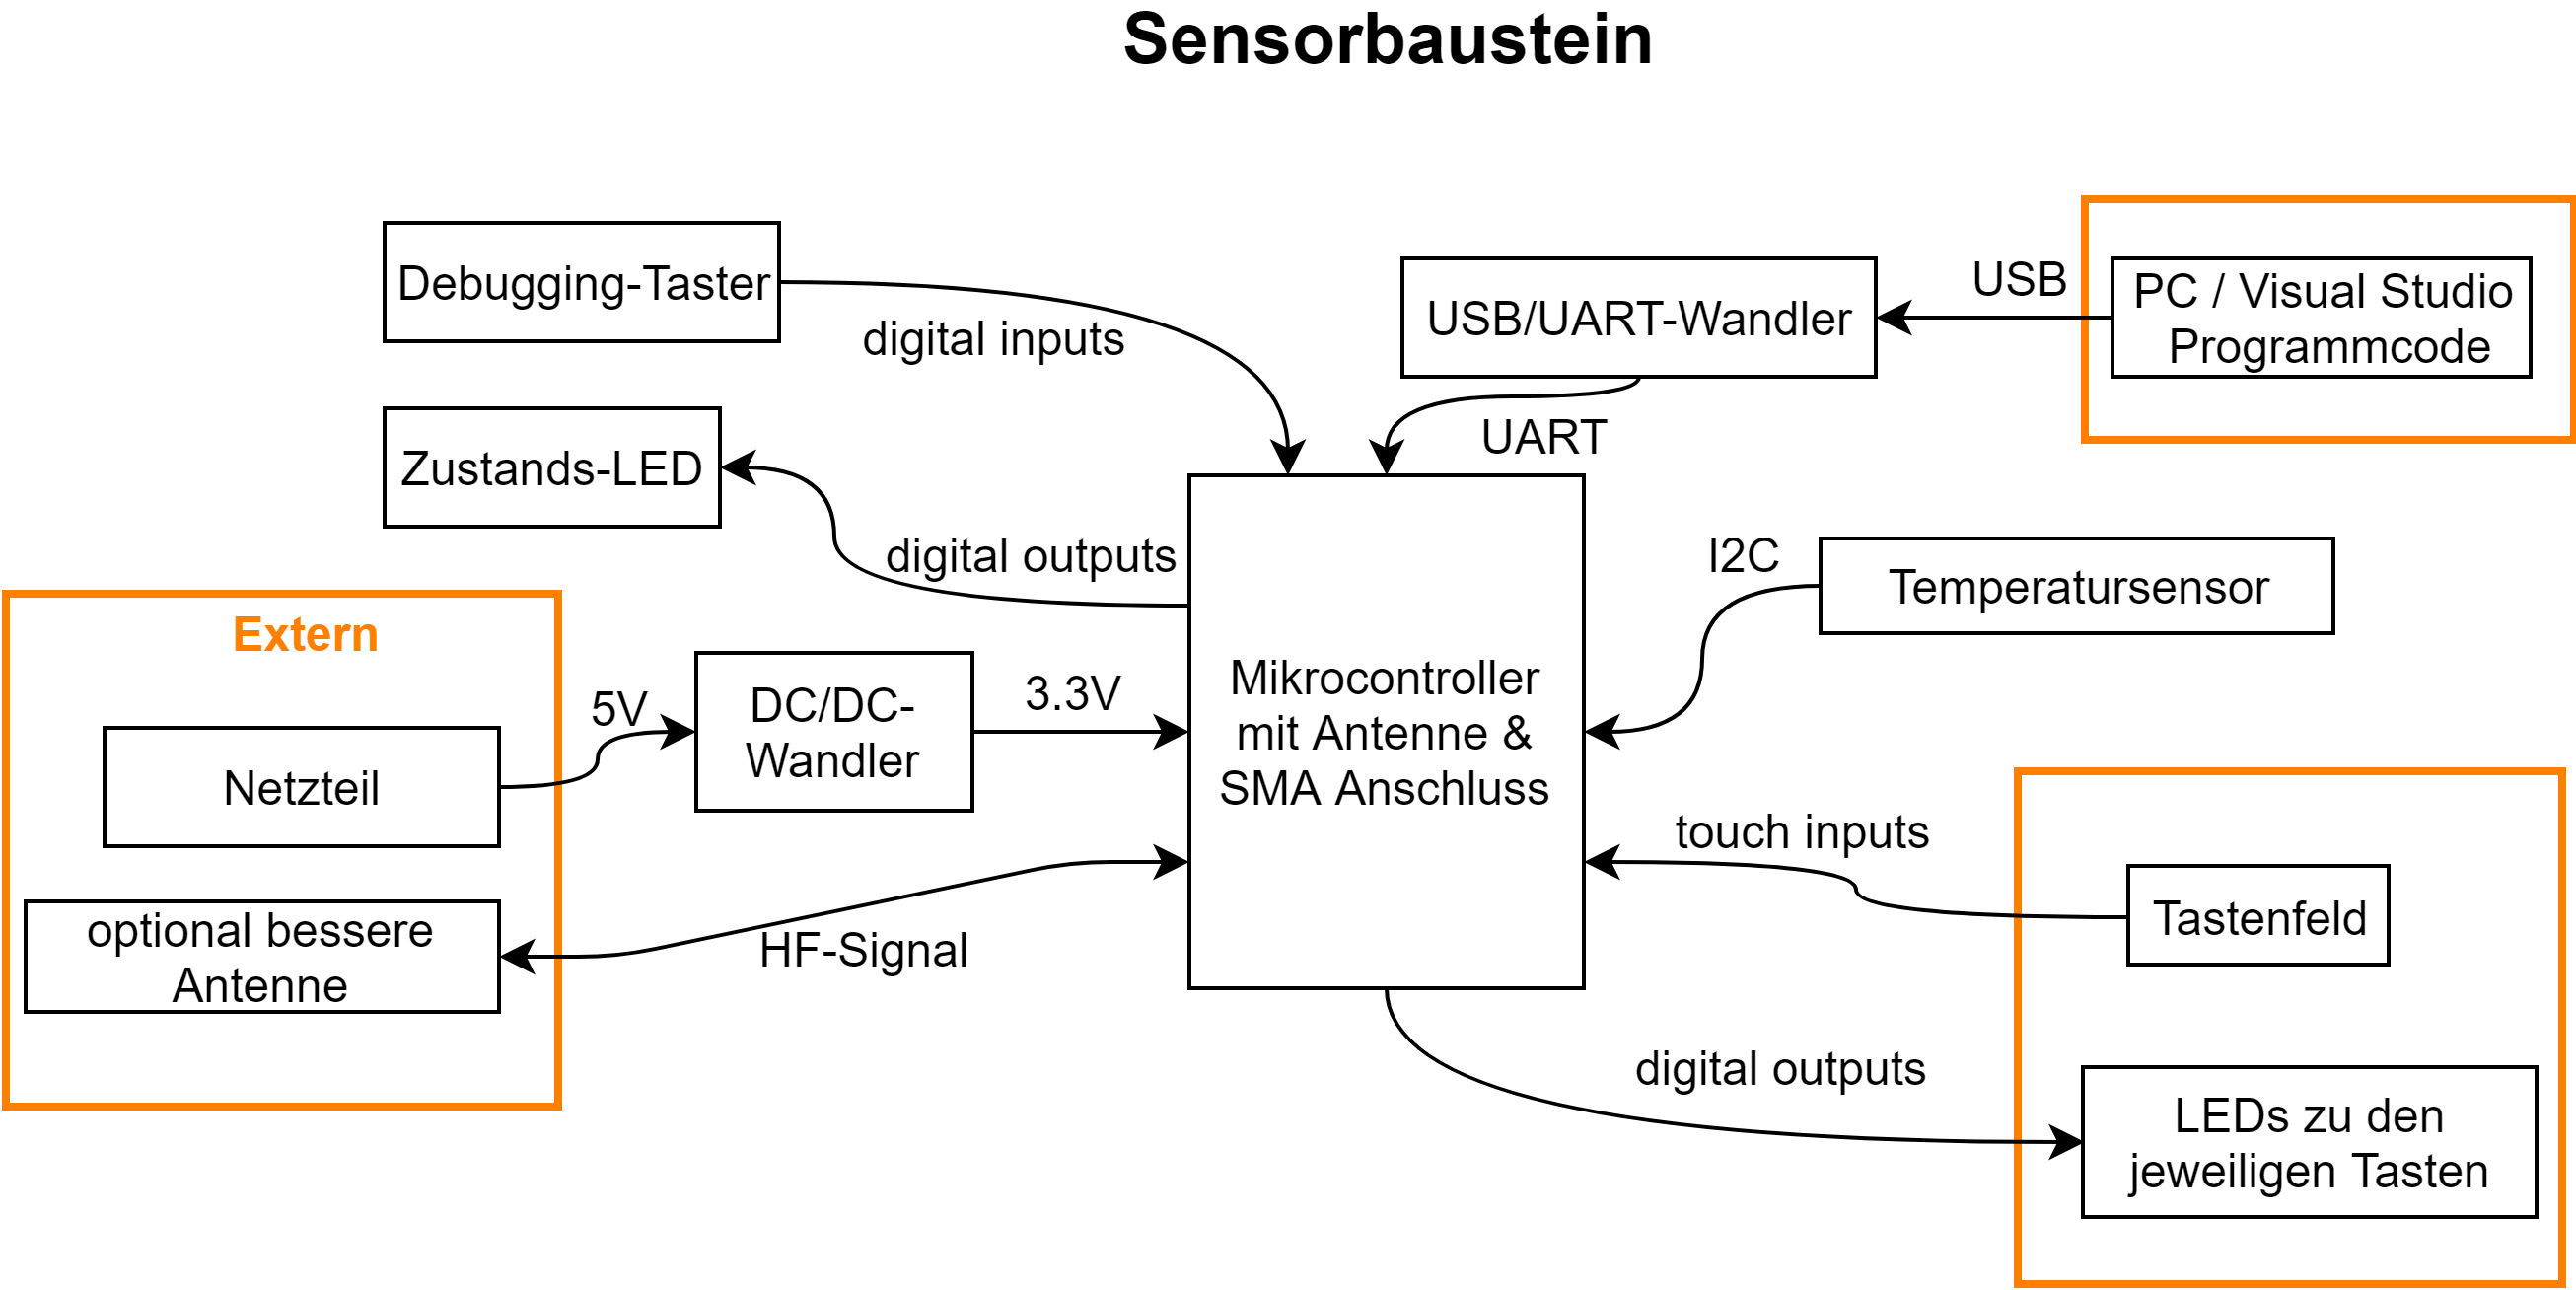
\includegraphics[width=\textwidth]{graphics/Sensorbaustein.png}
	\caption{Übersicht Sensorbaustein}
	\label{pic: Uebersicht_Sensorbaustein}
\end{figure} 

\subsubsection{Übersicht Frontplatte}
Die Frontplatte besteht aus einem 2-Lagen Print. Auf der Vorderseite (Abb. \ref{pic: Frontplatte_vorne}) sind vier runde Kupferflächen angebracht, welche als Touch Fläche fungieren. Wenn nun ein Anwender eine dieser Fläche berührt, wird die Kapazität zwischen dieser Fläche und Ground vergrössert. Natürlich befindet sich ein Lötstopplack zwischen Finger und Kupferfläche der Dielektrikum darstellt. Der ESP32 hat intern Touchsensoren verbaut, welche ein Signal auf auf die Pins geben und dann vermutlich mithilfe eines Spannungsteilers messen ob, dass Signal grösser oder kleiner wird. Zu den Tasten gibt es jeweils eine LED, welche von der Rückseite montiert werden. Der NTC ist auf der Rückseite der Frontplatte angebracht. Um die Temperatur der tatsächlichen Raumluft zu messen wurde auf der Frontplatte eine Kupferfläche auf der Aussenseite angebracht, welche die Wärme via Vias zum NTC weitergibt. Als Verbindung zur Hauptplatine des Sensorbausteins ist ein 12-Pin Stecker mit 2.54\,mm Rastermass vorgesehen. Eine Randnotiz: Es wurde darauf geachtet, dass keine visuell störenden Vias, das optische Erscheinungsbild beeinträchtigen.

\begin{figure}[h!]
	\centering
	\begin{minipage}[t]{0.4\linewidth}
	\centering
	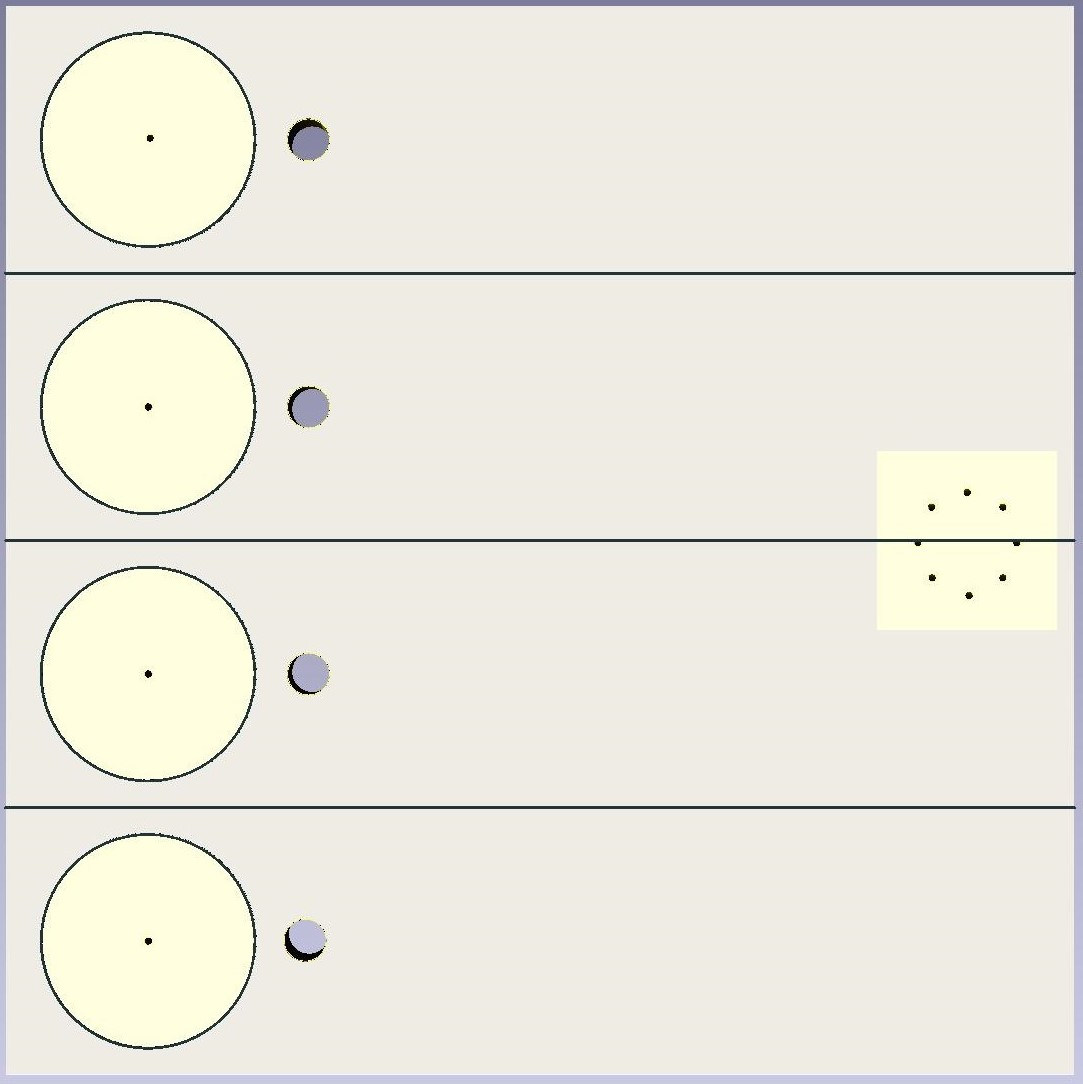
\includegraphics[width=1\textwidth]{graphics/Frontplatte_vorne.jpg}
	\caption{Frontplatte Vordersansicht}
	\label{pic: Frontplatte_vorne}
	\end{minipage}% <- sonst wird hier ein Leerzeichen eingefügt
	\hfill
	\begin{minipage}[t]{0.4\linewidth}
	\centering
	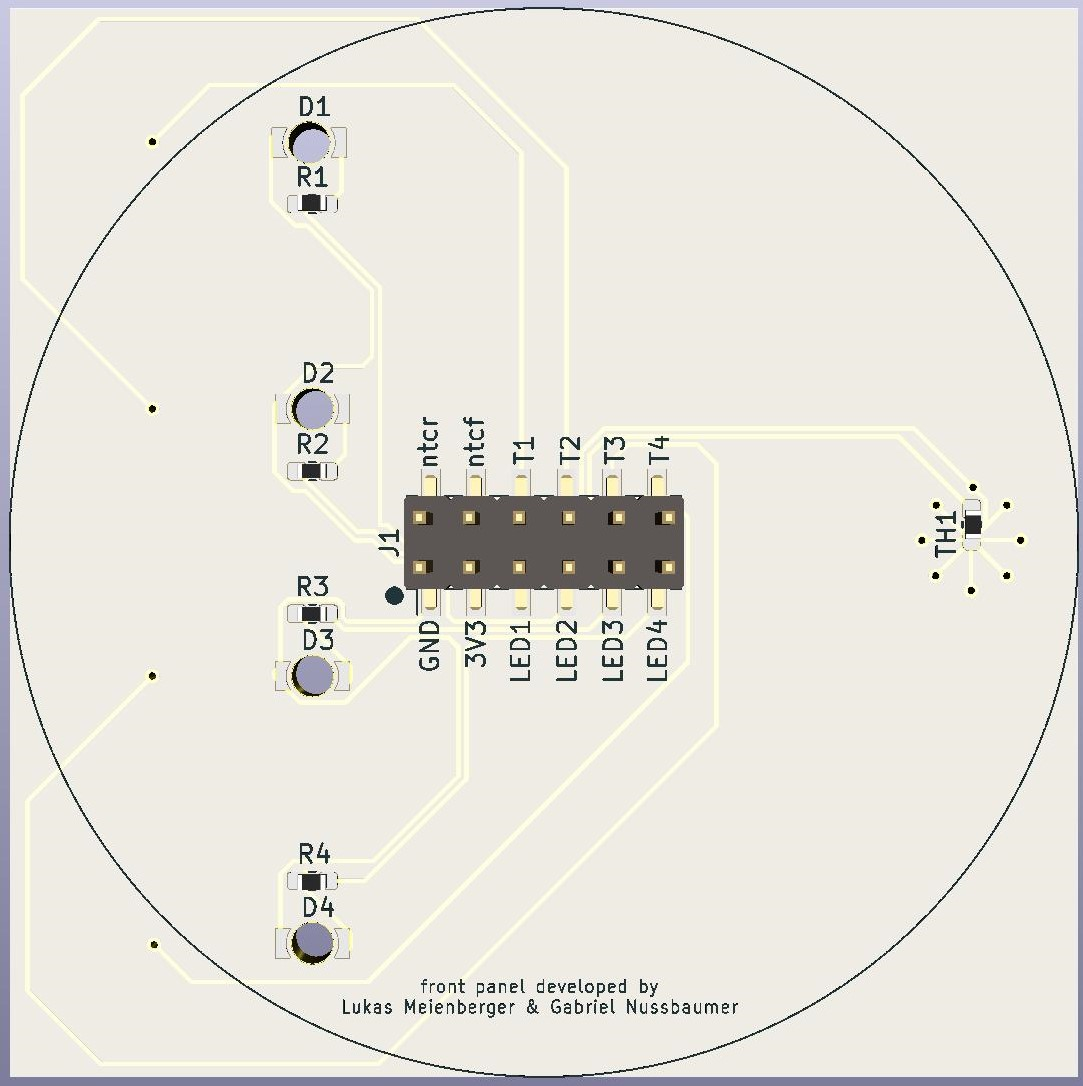
\includegraphics[width=1\textwidth]{graphics/Frontplatte_hinten.jpg}
	\caption{Frontplatte Rückansicht}
	\label{pic: Frontplatte_hinten}
	\end{minipage}
\end{figure}

\subsubsection{Übersicht Hauptplatine}
Auf der Vorderseite der Hauptplatine des Sensorbausteins (Abb. \ref{pic: Hauptplatine_vorne}) befindet sich der ESP32, der Programmieranschluss über USB und den 5V/3V Wandler. Über die Buchse kann dann die Frontplatte angeschlossen werden, wobei auf die Richtung geschaut werden muss. Auf der Rückseite (Abb. \ref{pic: Frontplatte_hinten}) Shottky-Dioden, welche bei einem allfälligen ESD auf den Touchflächen greiffen. Ebenso befinden sich dort Buttons, eine Status LED sowie 5V und RX/TX Anschlüsse. 

\begin{figure}[h!]
	\centering
	\begin{minipage}[t]{0.4\linewidth}
		\centering
		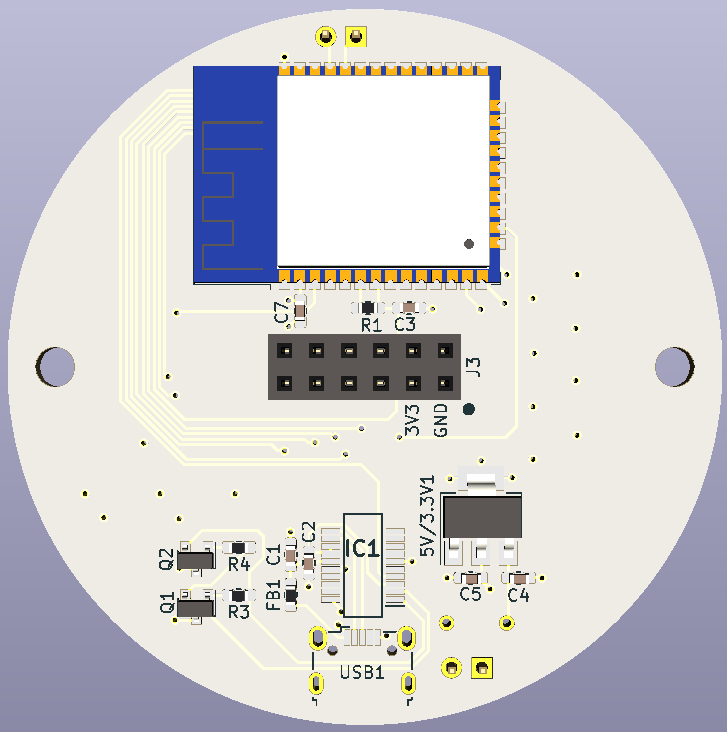
\includegraphics[width=1\textwidth]{graphics/Hauptplatine_vorne.png}
		\caption{Hauptplatine Vorderansicht}
		\label{pic: Hauptplatine_vorne}
	\end{minipage}% <- sonst wird hier ein Leerzeichen eingefügt
	\hfill
	\begin{minipage}[t]{0.4\linewidth}
		\centering
		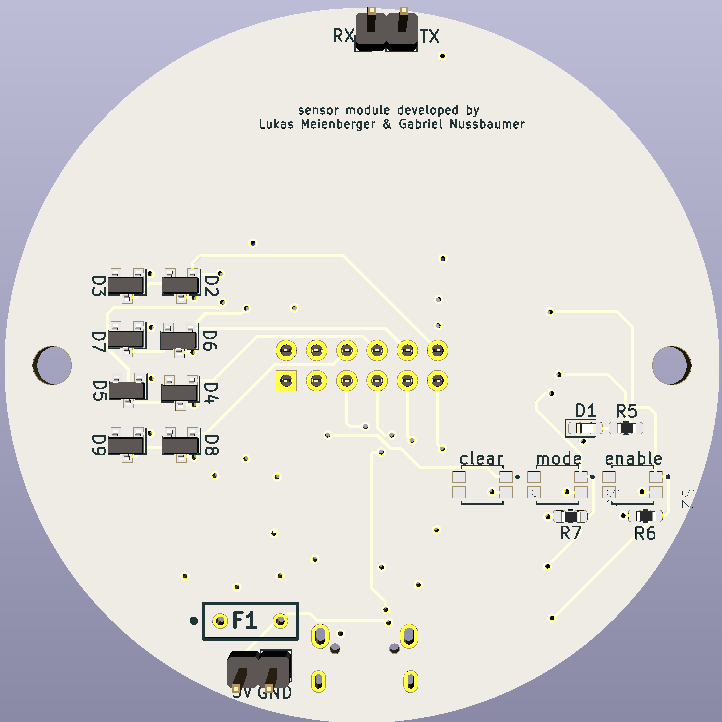
\includegraphics[width=1\textwidth]{graphics/Hauptplatine_hinten.png}
		\caption{Hauptplatine Rückansicht}
		\label{pic: Hauptplatine_hinten}
	\end{minipage}
\end{figure}


\subsubsection{Mikrocontroller}
\label{Hardware Mikrocontroller_Sensor}
Um die Datenkommunikation über WLAN bereitzustellen wird entweder ein ESP32-WROOM oder der ESP32S, welcher im gleichen Formfaktor zur integrierten Antenne auch einen SMA Anschluss bietet, verwendet. Der ESP32 unterstützt Wi-Fi im Bereich von 2.4 GHz bis ca. 2.5 GHz \cite{espressif_esp32-wroom-32_datasheet_en_2019}. Aus folgender Übersicht sind die zur Verfügung gestellten Ein-/Ausgänge des ESP32 zu entnehmen:
% Please add the following required packages to your document preamble:
% \usepackage{graphicx}
% Please add the following required packages to your document preamble:
% \usepackage{graphicx}
\begin{table}[h!]
	\centering
	\begin{tabular}{|c|c|}
		\hline
		\textbf{Name}                                                                          & \textbf{Anzahl} \\ \hline
		\begin{tabular}[c]{@{}c@{}}Analog-to-Digital Converter (ADC)\\   channels\end{tabular} & 18              \\ \hline
		SPI interfaces                                                                         & 3               \\ \hline
		UART interfaces                                                                        & 3               \\ \hline
		I2C interfaces                                                                         & 2               \\ \hline
		PWM output channels                                                                    & 16              \\ \hline
		Digital-to-Analog Converters (DAC)                                                     & 2               \\ \hline
		I2S interfaces                                                                         & 2               \\ \hline
		Capacitive sensing GPIOs                                                               & 10              \\ \hline
	\end{tabular}
	\caption{I/O Uebersicht}
	\label{tab: IO Uebersicht}
\end{table}
\\
Der ESP32 verfügt über alle benötigten Schnittstellen, die für den Sensorbaustein relevant sind. Im folgenden (Tabelle \ref{tab: IO Sensorbaustein}) sind die Inputs/Outputs des Mikrocontrollers (folglich Abb. \ref{pic: ESP32_sensor}), welcher im Sensorbausteins verwendet wird, aufgeführt:
\begin{table}[h!]
	\centering
	\begin{tabular}{|c|c|}
		\hline
		\textbf{Name}                                                                          & \textbf{Anzahl} \\ \hline
		digital outputs für LEDs                                                               & 5               \\ \hline
		digital inputs für Buttons                                                             & 3               \\ \hline
		\begin{tabular}[c]{@{}c@{}}Capacitive sensing GPIOs für Touch\\   Buttons\end{tabular} & 4               \\ \hline
		UART interface für Programmierung                                                      & 3               \\ \hline
		I2C interfaces für Temperatursensor                                                    & 3               \\ \hline
	\end{tabular}
	\caption{I/O Sensorbaustein}
	\label{tab: IO Sensorbaustein}
\end{table}
\\
\begin{figure}[h!]
	\centering
	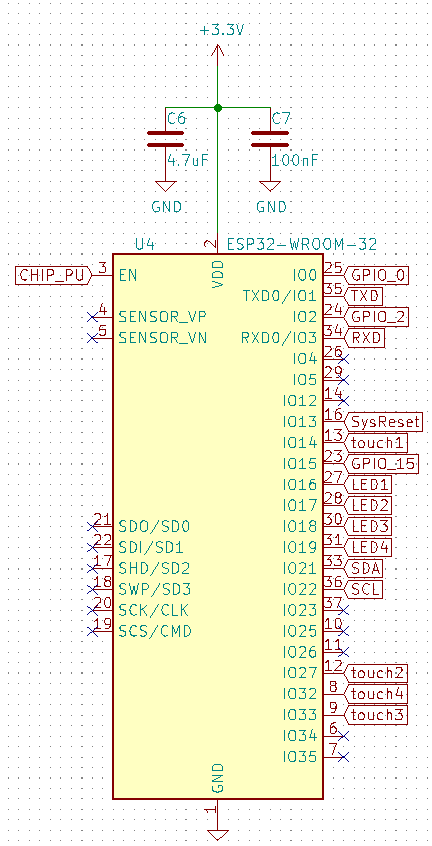
\includegraphics[width=0.5\textwidth]{graphics/shematics_sensor_ESP32.png}
	\caption{Mikrocontroller ESP32 im Sensorbaustein}
	\label{pic: ESP32_sensor}
\end{figure}
\subsubsection{Temperatursensor}
Es wird der NTC NCU18WF104J60RB von Murata Electronics verwendet. Dieser hat den preislichen Vorteil gegenüber anderen Varianten, wie ein Temperaturfühler IC. Der verwendete NTC hat eine B-Konstante von 4250\,K im Bereich 25/50\,°C mit einer Toleranz von 2\%. Der Widerstandswert des NTCs bei 25\,°C beträgt 100\,K mit einer Toleranz von 5\%. Um die Temperatur zu ermitteln wird ein Spannungsteiler (Abb. \ref{pic: Temperatursensor}) ist die verwendete Temperaturschaltung abgebildet. Das Signal ntc $_{ref}$ gibt eine Referenzspannung $U_{ref}$ mithilfe eines DACs aus, da der DAC ungenau ist, wird dieses Signal mithilfe von ntck eingelesen. Die Spannung über dem NTC $U_{ntc}$ wird mit ntcf gemessen und ntcr ist mit Ground verbunden, welches eine separate Rückleitung zur Hauptplatine des Sensorbausteins verfügt, um allfällige Störeinflüsse zu vermeiden. Die Temperatur wird berechnet indem als erstes der Widerstand des NTCs $R_T$ mit $R_T = \frac{U_{ntc}}{U_{ref}\;-\;U_{ntc}}$berechnet wird. Für $U_{ref}$ wird maximal eine Spannung von 2.5V verwendet, da der ADC danach nicht mehr linear ansteigt. Dann muss nur noch die Lineare Umrechnung des ADC wertes in eine Spannung beachtet werden. Die Temperatur in Kelvin ergibt sich dann aus $T = \frac{1}{\frac{1}{T_N}+\frac{1}{B} \cdot ln(R_T)}$.
\begin{figure}[h!]
	\centering
	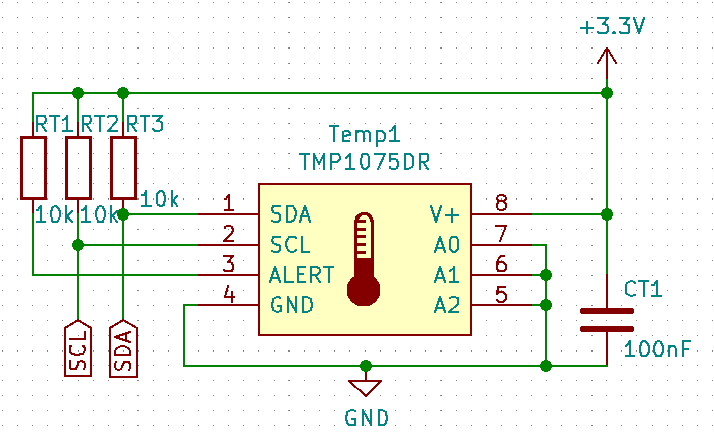
\includegraphics[width=0.5\textwidth]{graphics/shematics_sensor_Temp.png}
	\caption{Schaltung Temperatursensor}
	\label{pic: Temperatursensor}
\end{figure}

\subsubsection{Programmieranschluss}
\label{par: Programmieranschluss}
Der Mikrocontroller kann mittels eines USB to UART Wandlers programmiert werden. Hierzu wird der CP2104 verwendet. In Abbildung \ref{pic: USB Anschluss} ist das Schema abgebildet. Auf dem Schema sind dabei zwei Beipolartransistoren zu erkennen welche es erlauben den ESP32 ohne drücken des Modetasters in den Programmiermodus zu versetzen. Falls es zu Komplikationen kommt steht aber auch die Option mittels des Enable- und Mode-Buttons (Abb. \ref{pic: sensor_progrmmierbuttons}) sich in den Programmiermodus zu versetzen offen. Im Aktorbaustein befindet sich die gleiche Schaltung wieder. Falls man einen Systemreset machen möchte kann man den Clear Button betätigen. Die LED5 zeigt mittels eines kurzen Blinkens das Aufstarten des ESP32 an oder oder dass der ESP32 im Programmiermodus ist.
\begin{figure}[h!]
	\centering
	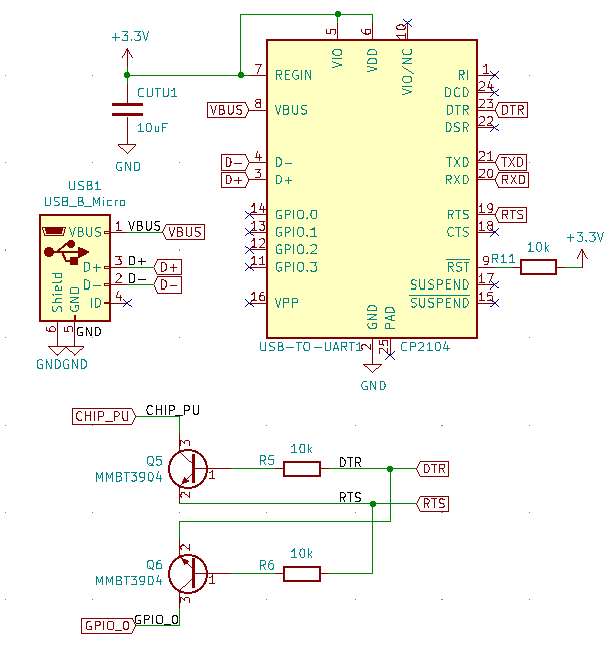
\includegraphics[width=0.75\textwidth]{graphics/shematics_usb.png}
	\caption{USB Anschluss}
	\label{pic: USB Anschluss}
\end{figure}
\begin{figure}[h!]
	\centering
	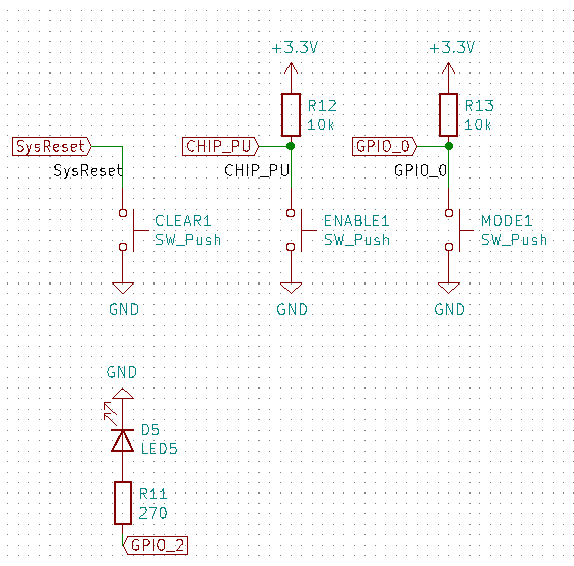
\includegraphics[width=0.6
	\textwidth]{graphics/shematics_sensor_buttons_LED.png}
	\caption{Buttons und LED auf Sensorbaustein}
	\label{pic: sensor_progrmmierbuttons}
\end{figure}
\subsubsection{Spannungsversorgung}
Der minimale Strom, welche die Spannungsquelle zur Verfügung stellen muss sind laut Datenblatt vom ESP32 500 mA, wobei im Normalbetrieb 80 mA und im WiFi Sendebtrieb 160 mA bis 260 mA gebraucht werden.
Um den Sensorbaustein mit 5 V zu versorgen, macht es aus Platz gründen Sinn den 230 V/AC zu 5 V/DC Wandler separat und nicht auf der Leiterplatte zu haben. Hier kommt beispielsweise der Mean Well RS-15-5 AC/DC infrage, welcher 90 V/AC bis 264 V/AC zu 5 V/DC bei max. 15 W bzw. 3 A wandeln kann. Dieser kostet bei Digi-Key momentan 9.47 Fr und ist noch dem unteren Preissegment zugeordnet, was aber immer noch relativ teuer ist im Vergleich zu den restlichen Komponenten. Da der Wandler separat zur Leiterplatte ist kann er jedoch immer noch im Nachhinein durch einen günstigeren mit vielleicht weniger Leistung ca. 5 W ausgetauscht werden.
Der Mikrocontroller benötigt 3.3 V, jedoch soll der Sensorbaustein mit 5V betrieben werden können. Hierfür wird einen Spannungswandler eingesetzt. Der ausgewählte AP1117S33CTR hat einen maximale Input Spannung von 15V, eine maximale Dropoutspannung von 1.2 V bei 800mA und ist, mit momentan 0.42\$ bei Digi-Key, günstig. Im Schema (Abb. \ref{pic: Wandler_Sensor}) erkennt man, dass sowohl über USB wie auch über einen Stecker den Print mit 5 V versorgt werden können. Eingebaut ist eine Sicherung die verhindern soll, dass bei einem Kurzschluss der Sensorbautein anfängt grossen Schaden zu nehmen oder schlimmeres.
\begin{figure}[h!]
	\centering
	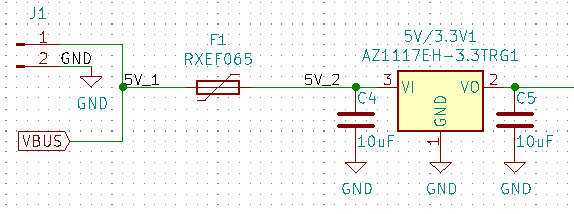
\includegraphics[width=0.7\textwidth]{graphics/shematics_sensor_33V.png}
	\caption{Spannungswandler Sensorbaustein}
	\label{pic: Wandler_Sensor}
\end{figure}
\subsubsection{Interface}
Der Sensorbaustein wird Taster und dazugehörige LEDs beinhalten, jedoch macht es Sinn diese auf einen separaten Print zur Verfügung zu stellen. Gründe hierfür sind der begrenzte Platz auf dem Hauptprint, separater Print kann als Frontplatte verwendet werden und bessere Integration der LEDs. Angedacht ist eine Frontplatte welche Touchsensoren, diese sind nichts anderes als dicke Leiterbahnen, beinhalten. Das einlesen der Touchsensoren gestaltet sich mit dem ESP32 äusserst einfach und läuft unabhängig vom WiFi, dies sei gesagt weil es z.B. Probleme gibt wenn der ADC2 und das WiFi gleichzeitig benutzt werden. Die LEDs könnten dann rückwärts montiert (reverse mounted LEDs) werden, welche durch die Leiterdplatte hindurchläuchten. In der Abbildung \ref{pic: Stecker_Sensor} sind die Steckverbindungen abgebildet, welche jeweils aus 4 Stecker für den Touch und LEDs bestehen, dazu kommen noch 3.3 V und GND Stecker sowie GPIO2, GPIO15, RXD und TXD Stecker, welche nützlich sind wenn man den Mikrocontroller über diese Schnittstelle programmieren oder einfach eine Verbindung haben möchte.
\begin{figure}[h!]
	\centering
	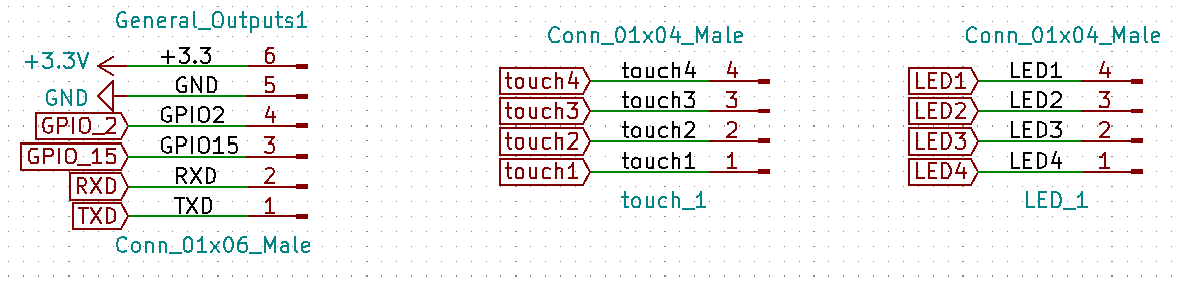
\includegraphics[width=0.8\textwidth]{graphics/shematics_sensor_stecker.png}
	\caption{Steckverbindungen Sensorbaustein}
	\label{pic: Stecker_Sensor}
\end{figure}
\subsubsection{Platzstudie}
Nun wird mittels einer Platzstudie überprüft ob der Sensorbaustein, mit den verwendeten Komponenten, wie eine Unterputzsteckdose eingebaut werden kann.
Im Bild \ref{pic: Montageplatte.png} ist eine Montageplatte für UP-Steckdosen abgebildet. Der blaue Kreis Zeigt dabei den Radius von 60 mm des Tasters bzw. Kleinkombination. Diese Masse wurden für die Dimensionen der Platine in Abbildung \ref{pic: pcb_sensor_dimensionen.png} übernommen. Abbildung \ref{pic: pcb_sensor_vorne} und \ref{pic: pcb_sensor_hinten} zeigen, wie die Komponenten auf der begrenzten Platine angeordnet werden können.

\begin{figure}[htb]
	\centering
	\begin{minipage}[t]{0.45\linewidth}
		\centering
		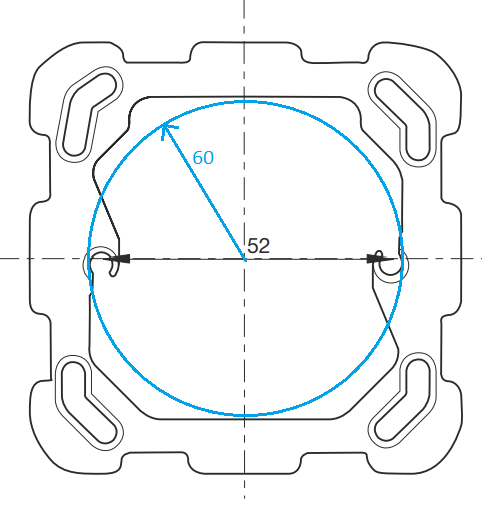
\includegraphics[width=0.9\textwidth]{graphics/Montageplatte.png}
		\caption{Montageplatte \cite{hager_hager_kat1_08_technik_d_2019} }
		\label{pic: Montageplatte.png}
	\end{minipage}% <- sonst wird hier ein Leerzeichen eingefügt
	\hfill
	\begin{minipage}[t]{0.45\linewidth}
		\centering
		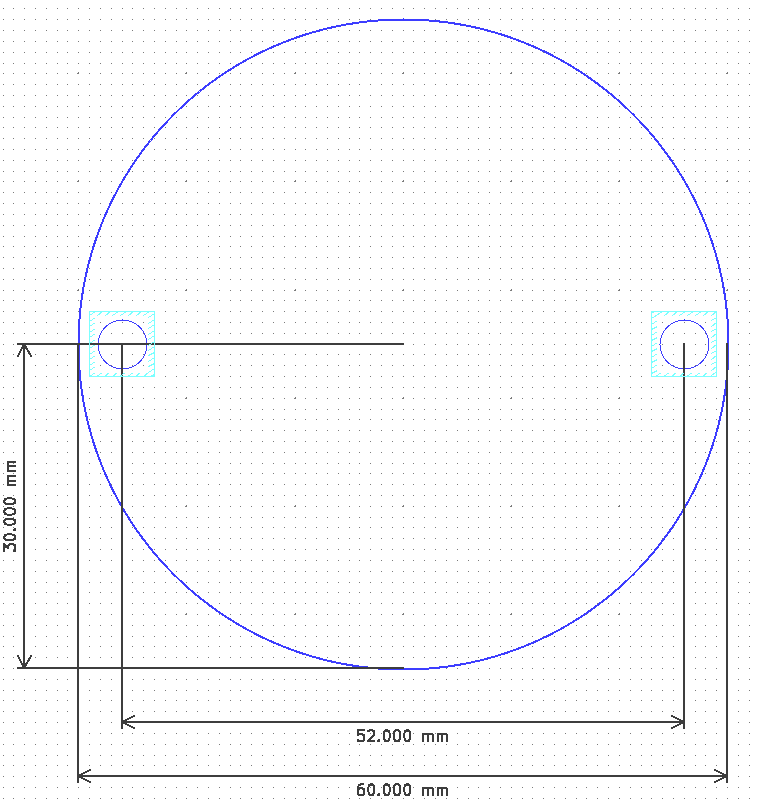
\includegraphics[width=0.90\textwidth]{graphics/pcb_sensor_dimensionen.png}
		\caption{PCB Sensorbaustein Dimensionen}
		\label{pic: pcb_sensor_dimensionen.png}
	\end{minipage}
\end{figure}

\begin{figure}[htb]
	\centering
	\begin{minipage}[t]{0.45\linewidth}
		\centering
	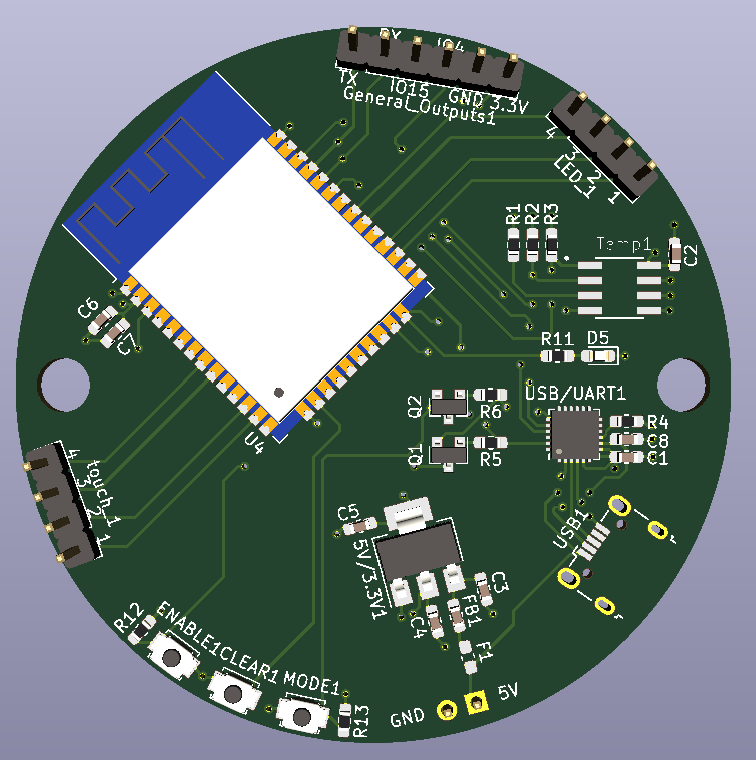
\includegraphics[width=0.90\textwidth]{graphics/pcb_sensor_vorne.png}
\caption{PCB Sensorbaustein von vorne}
\label{pic: pcb_sensor_vorne}
	\end{minipage}% <- sonst wird hier ein Leerzeichen eingefügt
	\hfill
	\begin{minipage}[t]{0.45\linewidth}
		\centering
	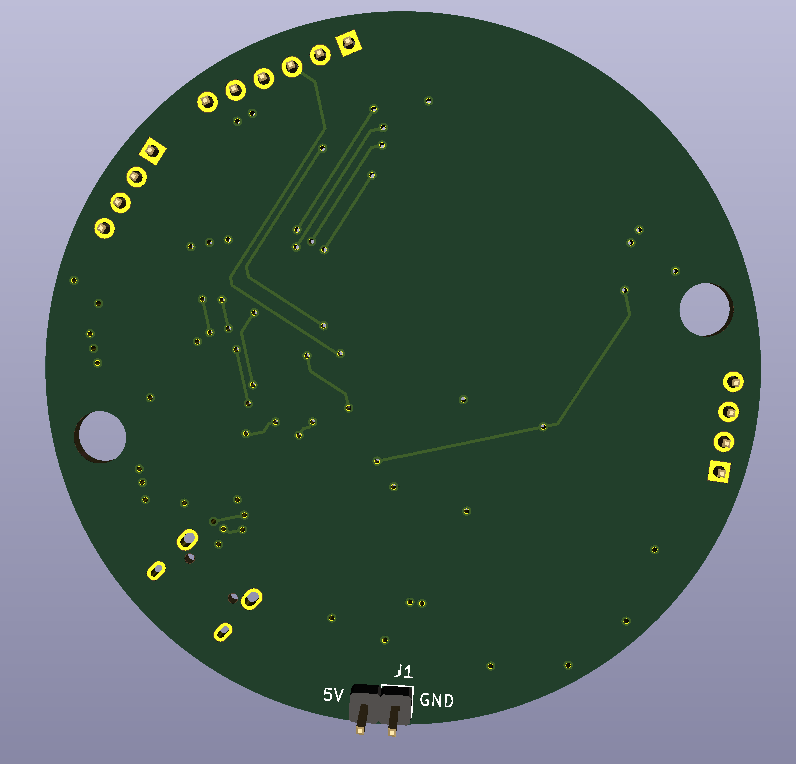
\includegraphics[width=0.90\textwidth]{graphics/pcb_sensor_hinten.png}
\caption{PCB Sensorbaustein von hinten}
\label{pic: pcb_sensor_hinten}
	\end{minipage}
\end{figure}






 \newpage
\subsection{Aktorbaustein}\label{subsec: Aktorbaustein}
Im folgenden wird die Hardware des Aktorbausteins, ähnlich wie beim Sensorbaustein, beschrieben. Vom Auftraggeber ist ein Aktorbaustein mit 4 Relais, zwei Ausgängen $0..10\;V$ und zwei Eingängen $0..10\;V$ gefordert. Der Aktorbautein wird über 24V-Netzteil mit Spannung versorgt und mithilfe eines On-Off Schalters kann die Spannungsversorgung getrennt werden. Die Logik wird mit 3.3 V betrieben, dazu braucht es ein DC/DC Wandler der die 24 V in 3.3 V wandelt. Die Programmierschnittstelle ist dabei gleich wie beim Sensorbaustein (siehe Kapitel \ref{sec: Sensorbaustein}). Die Spannung der  0...10 V Ausgänge werden über PWM eingestellt und bei den 0...10 V Eingängen kommt der AD-Wandler des Mikrocontrollers zum Einsatz. Damit man weiss welche Relais geschaltet haben, werden LEDs zum Signalisieren verwendet. Um eine bessere Funkreichweite zu erzielen, kann bei dem Aktorbautein, wie beim Sensorbautein, eine Antenne angebracht werden, angedacht ist die Verwendung einer zertifizierten Dipolantenne.
In der Abbildung \ref{Aktorbaustein_Ansicht} erkennt man rechts oben die vier Relais mit den jeweiligen LEDs unten dran. Rechts unten sind die zwei Eingänge und links davon die Ausgänge.


\begin{figure}[h!]
	\centering
	\includegraphics[width=\textwidth]{graphics/Aktorbaustein_Ansicht.png}
	\caption{Frontansicht des Aktorbausteins}
	\label{Aktorbaustein_Ansicht}
\end{figure} 

\begin{figure}[h!]
	\centering
	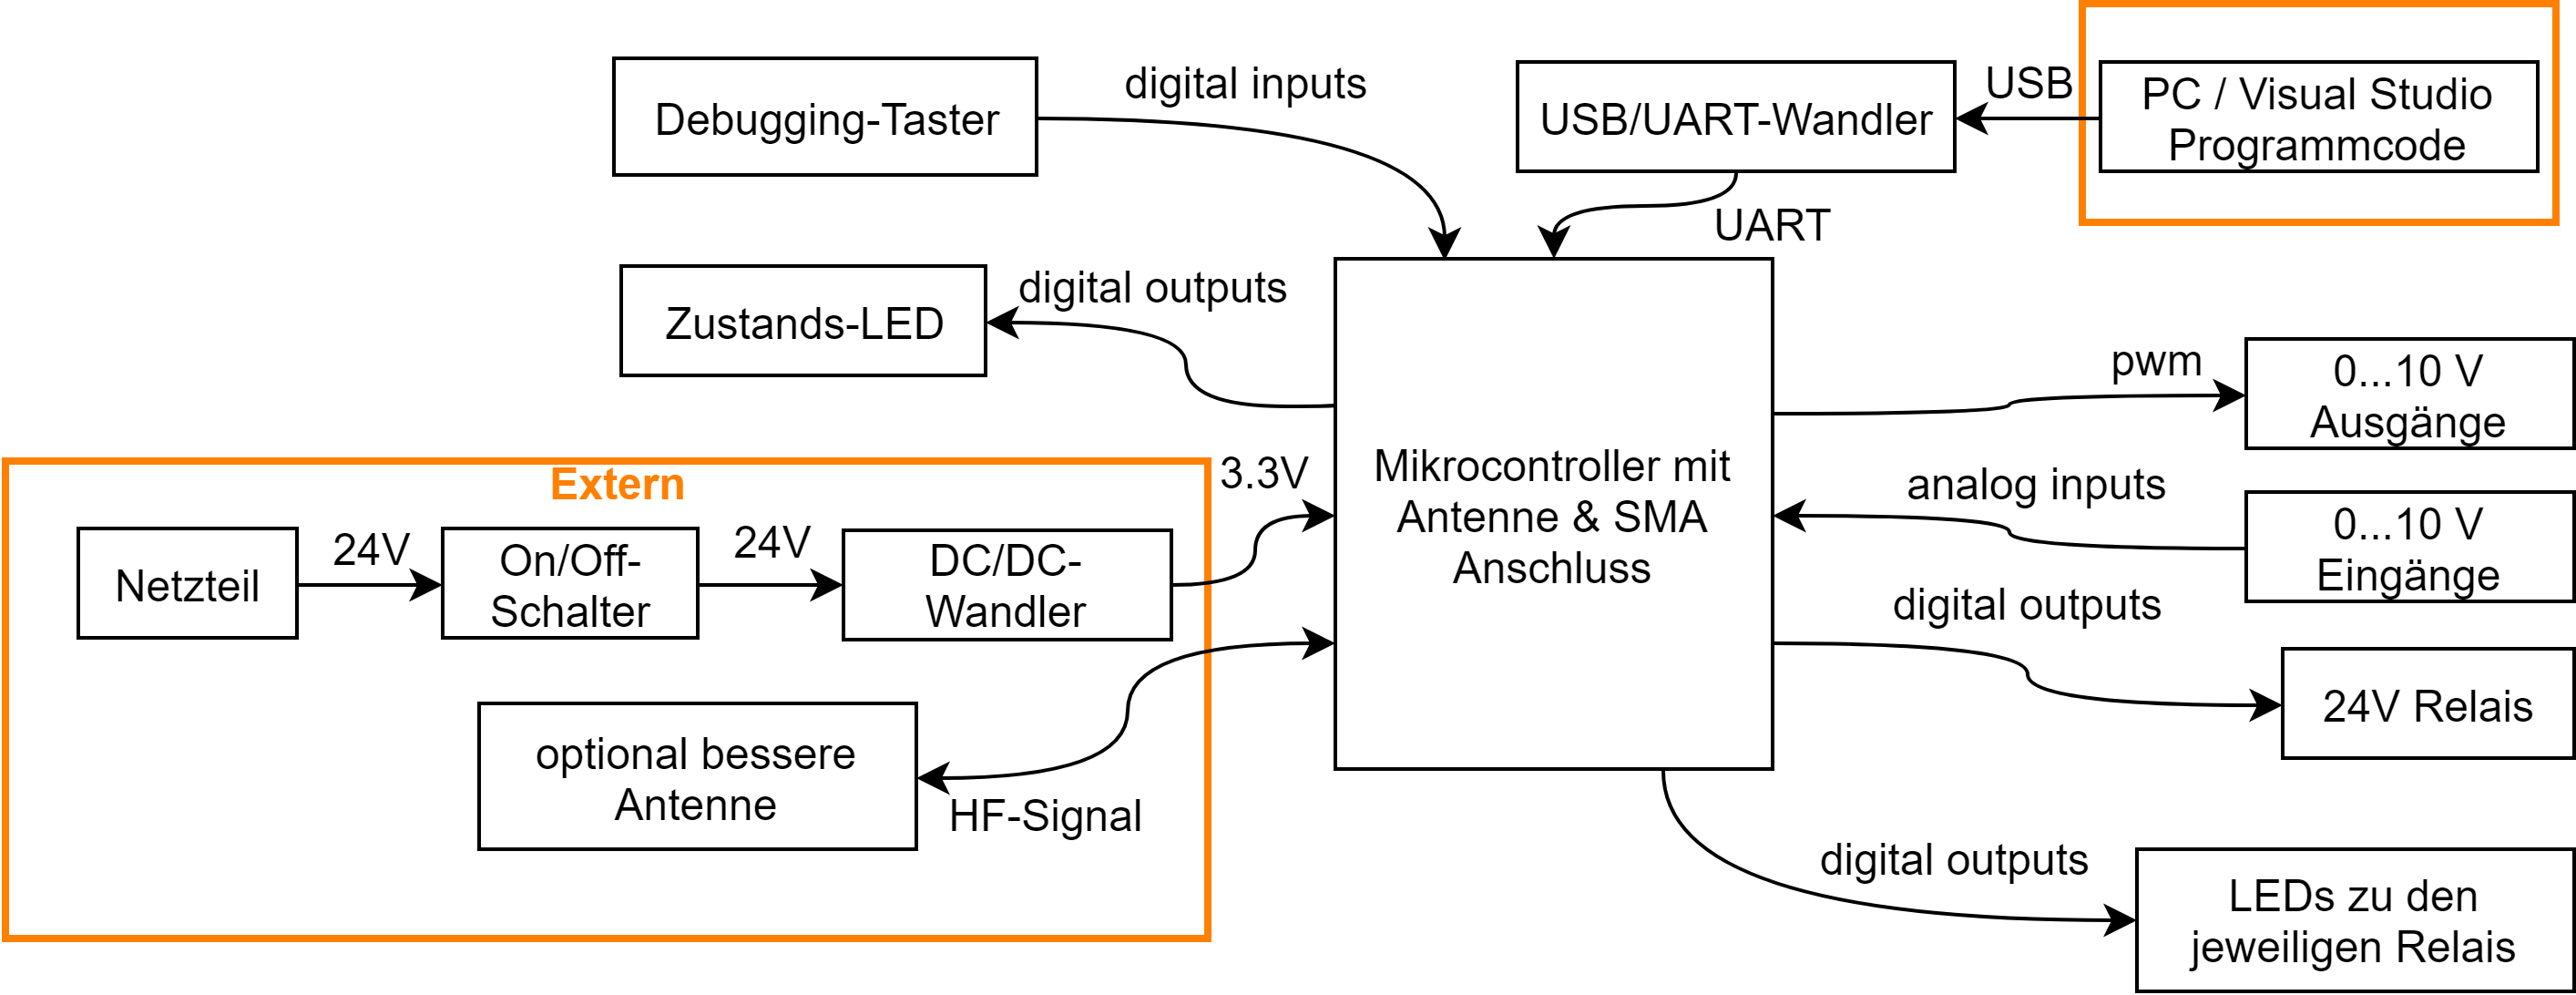
\includegraphics[width=\textwidth]{graphics/Aktorbaustein.png}
	\caption{Übersicht des Aktorbausteins}
	\label{pic: Uebersicht_Aktorbaustein}
\end{figure} 

\subsubsection{Mikrocontroller}\label{Hardware Mikrocontroller_Aktor}
Es wird wie schon im Sensorbaustein den ESP32 verwendet, dadurch kann garantiert werden, dass die WiFi-Systeme sich sowohl im Aktor- wie auch im Sensorbaustein sich in etwa gleich verhalten, wodurch der Entwicklungsaufwand minimiert wird. Die vom ESP32 benötigten I/Os werden in der Tabelle \ref{tab: IO Aktorbaustein} aufgelistet und in der Abbildung \ref{pic: ESP32_aktor} erkennt man welche I/Os verwendet wurden. Der Programmieranschluss ist wie beim Sensorbaustein und wird nicht nochmals wiederholt.
\begin{table}[h!]
	\centering
	\begin{tabular}{|l|l|}
		\hline
		\textbf{Name}                      & \textbf{Anzahl} \\ \hline
		digital outputs für Relais \& LED  & 10              \\ \hline
		digital inputs für Buttons         & 3               \\ \hline
		ADC inputs für \glqq $10\;V$\grqq Eingänge  & 2      \\ \hline
		PWM outputs für \glqq$10\;V$\grqq Ausgänge & 2       \\ \hline
		UART Interface für Programmierung  & 3               \\ \hline
	\end{tabular}
	\caption{I/O Aktorbaustein}
	\label{tab: IO Aktorbaustein}
\end{table}
\begin{figure}[h!]
	\centering
	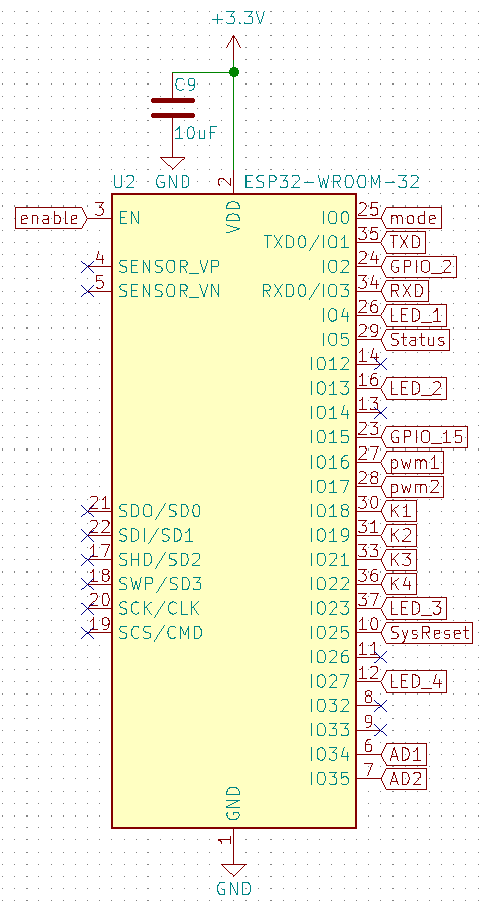
\includegraphics[width=0.45\textwidth]{graphics/shematics_aktor_ESP32.png}
	\caption{Mikrocontroller ESP32 im Aktorbaustein}
	\label{pic: ESP32_aktor}
\end{figure}


\subsubsection{Relais}
Die Anforderungen an ein Relais sind, dass es $230\,VAC$ schalten und die Relaisspule mit $24\,VDC$ betrieben werden muss. In der Abbildung \ref{pic: Relais_aktor} ist die Schaltung für ein Relais abgebildet. Als Relais wird ein G5LE-1-VD DC24 von Omron Electronics verwendet, welches mit den oben gennanten Anforderungen kompatibel ist. Der maximale Schaltstrom beträgt 10\,A und die maximale Schaltspannung 250\,VAC oder 125\,VDC. Die Nennspannung der Spule beträgt 24\,VDC, dabei ist garantiert, dass die Spule noch bei 75\,\% also 18\,V der Nennspannung anzieht und bei sicher 10\,\% der Nennspannung also 2.4\,V loslässt. Mit dem Widerstand $R_1$ wird der Einschaltstrom auf $10\;mA$ begrenzt, mithilfe der Freilaufdiode D1 kann die Selbstinduktionsspannung der Spule kurzgeschlossen werden und $R_{24}$ ist ein Pull-Down-Widerstand, so dass der MOSFET sicher sperrt, falls der Output-Pin nicht angesteuert wird \cite{mikrocontroller.net_relais_nodate}. Als MOSFET wird der BSS123 eingesetzt, welcher sich typischerweise schon mit einer Steuerspannung von $1.7\,V$ durchschaltet und eine Drain-Source-Spannung von bis zu $100\,V$ vertragen kann. Um Energie zu sparen wird nach dem anziehen der Spule mittels eines PWMs die mittlere Spannung über der Spule gesenkt, ein kurzer Test hat ergeben, dass die verwendeten Relais bei 30\,\% der Nennspannung also 7.2\,V sicher noch anziehen, was bedeutet, dass die Leistung von 400\,mW auf 36\,mW gesenkt wird.
\begin{figure}[h!]
	\centering
	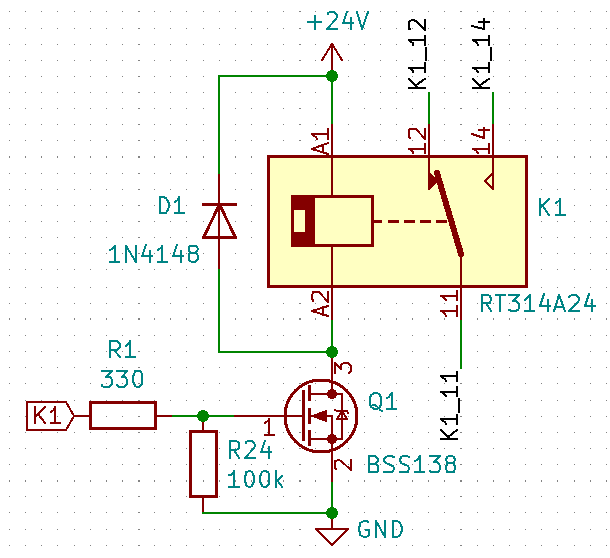
\includegraphics[width=0.45\textwidth]{graphics/shematics_relais.png}
	\caption{Relais im Aktorbaustein}
	\label{pic: Relais_aktor}
\end{figure}

\subsubsection{Eingänge}
Die $10\;V$ Eingänge werden mittels Varistoren (AMCV-0402-260-C180N-T) und Shottky-Dioden vor Überspannung geschützt (Abb. \ref{pic: Input_aktor}) Überspannungen können entstehen, wenn eine lange Signalleitung verwendet wird, welche induktiv wirkt und dann abgeschaltet wird. Die Nennspannung des Varistors beträgt 18.4\,VAC bzw. 26\,VDC, mit einer Varistorspannung von 31\,V bis 38\,V. Darunter schützen die Shottky-Dioden den ADC-Eingang. Falls der der Varistor zerstört wird, wird er leitend und es entsteht ein Kurzschluss am Eingang, was zu falschen Messresultaten führt. Auf Grund dessen, dass der ADC (Abbildung: \ref{pic: ESP32_Kurve}), erst ab 170\,mV ein Signal erkennt, muss ein Widerstandsnetzwerk verwendet werden. Hierdurch können auch niedrigere Spannungen gemessen werden können. Es wurde in der Gleichung \ref{eq: U_AD1} die Übertragungsfunktion des Wiederstandnetzwerkes ausgerechnet, durch den Offset ist es nun theoretisch möglich 0\,V zu messen. Es wurde eine variable Spannung mit 1\,\% Toleranz an die 10\,V Eingänge des Aktorbausteins gelegt und dann der ADC-Wert aufgenommen (Abbildung \ref{pic: /ADC_Input_Kurve}). Die so erstellte Regressionsgerade $U_{AD,measure}$ unterscheidet sich von der theoretisch berechneten Gerade $U_{AD1}$.

\begin{align}
U_{AD1} &= U_{in1} \cdot \frac{R_{23}||R_{24}}{R_{21}+R_{23}||R_{24}} + 3.3\,V \cdot \frac{R_{33}||R_{24}}{R_{23}+R_{33}||R_{24}} =  U_{in1} \cdot 0.2339 + 0.2123\,V \label{eq: U_AD1}\\
ADC &= U_{AD1} \cdot 1253.1 - 218.54 = (U_{in1} \cdot 0.2339 + 0.2123\,V) \cdot 1253.1 \frac{1}{V} - 218.54\\
ADC &= U_{AD1} \cdot 293.1 \frac{1}{V} + 47.5\\
U_{AD1} &= 0.003412\,V \cdot ADC - 0.162\,V\\
U_{AD,measure} &= 0.003449\,V \cdot ADC - 0.276\,V
\end{align}

\begin{figure}[h!]
	\centering
	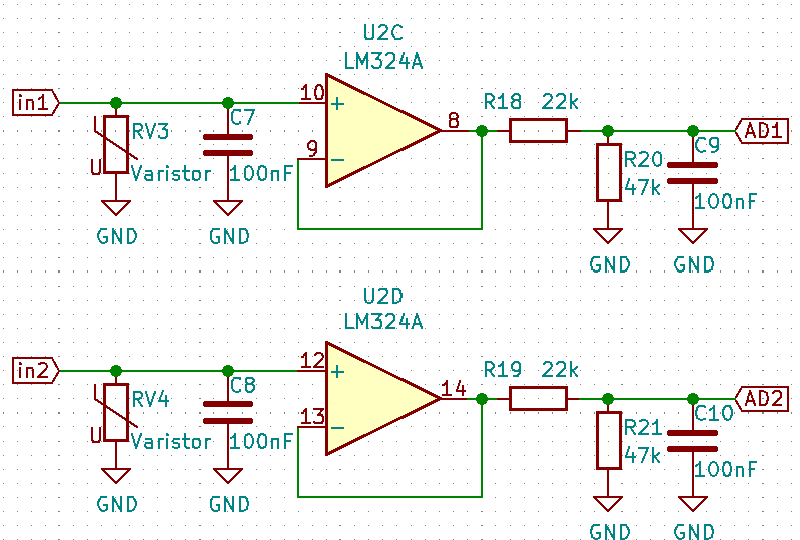
\includegraphics[width=0.5\textwidth]{graphics/shematics_aktor_input.png}
	\caption{10\,V Eingänge des Aktorbausteins}
	\label{pic: Input_aktor}
\end{figure}

\begin{figure}[h!]
	\centering
	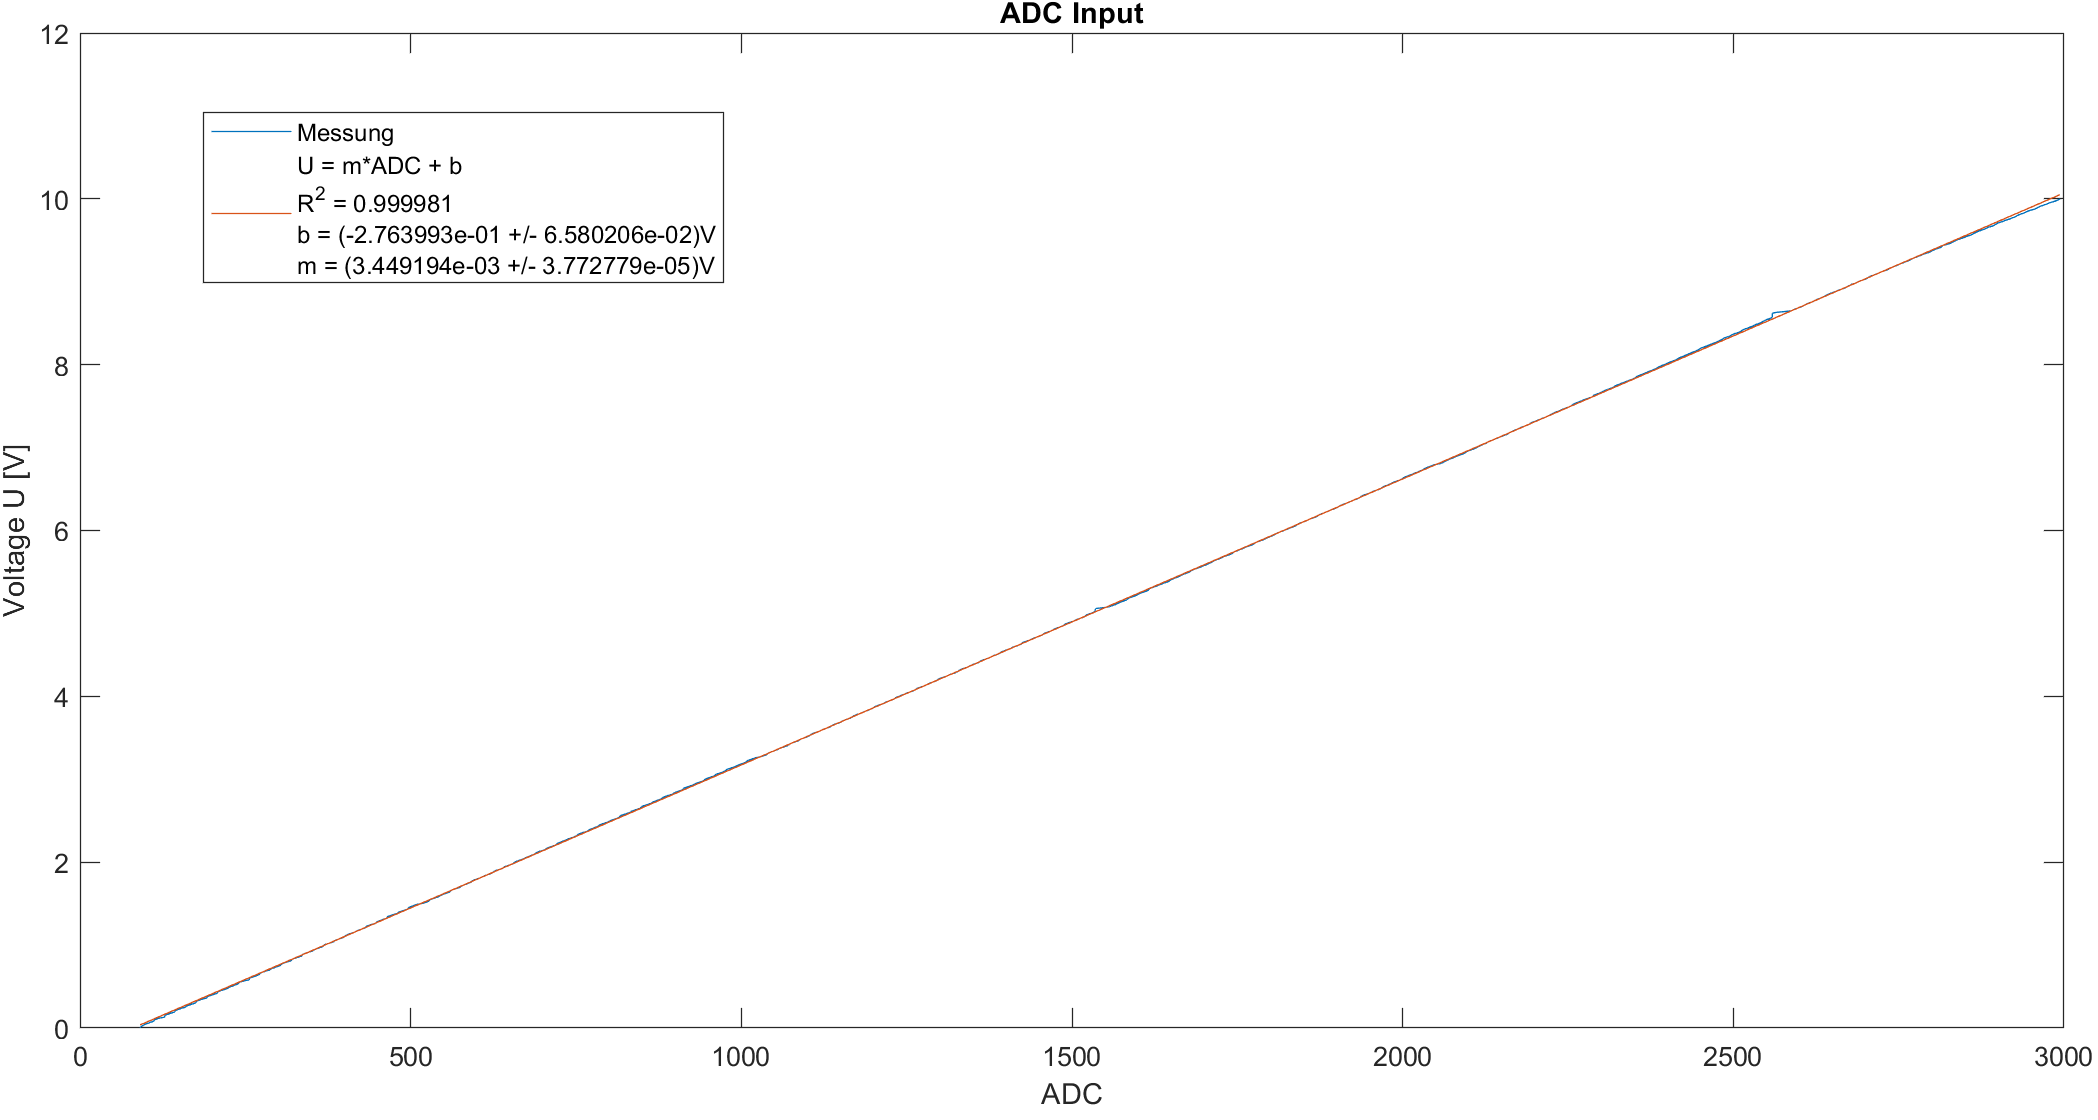
\includegraphics[width=1\textwidth]{graphics/ADC_Input_Kurve.png}
	\caption{Spannung gegenüber dem ADC Wert gemessen an beiden 10\,V Eingängen und dann gemittelt}
	\label{pic: /ADC_Input_Kurve}
\end{figure}
\newpage
\subsubsection{Ausgänge}
Bei den $10\;V$ Ausgängen wird jeweils ein PWM vom Mikrocontroller herausgegeben und dann das Signal mittels eines Tiefpasses geglättet (Abb. \ref{pic: Output_aktor}). Die Polfrequenz sowie die $-3dB$ Grenzfrequenz des Tiefpass erster Ordnung berechnet sich für einen 10 Bit AD Wandler und einen Quarz von $40\;MHz$, welcher im ESP32 verbaut ist, folgendermassen: $40\;MHz$ Takt --> $40\;kHz$ PWM --> Zeitkonstante $\tau = 1000/40\;kHz = 25\;ms $ --> Zeit bis zum Endwert $ t_{end}=\tau * ln(1024) = 173\;ms$ --> Grenzfrequenz $f_g = 1/\tau = 40\;Hz$. Die Verzögerungszeit $t_{end}$ ist im Übrigen gleich der Dauer bis die Spannung am Kondensator im Bereich von 1 LSB vom Endwert ist \cite{ronald_locher_2017}. $173\;ms$ Verzögerungszeit scheinen recht lange zu sein, wenn man diese Zeit verkürzen möchte, könnte man auf einen 8 Bit AD Wandler wechseln, wodurch die Polfrequenz auf $156\;kHz$ angehoben wird. Ein anderer Weg besteht darin eine höhere Filterordnung zu wählen. Um eine Abschwächung von 1024 oder 60 dB des $40\;kHz$ PWM Taktes zu erzielen, kann bei zweiter Filterordnung, welche $40\;dB/dec$ Dämpfung hat, die $40\;kHz$ nicht durch 3 Dekaden (Faktor 1000) sondern nur um 1.5 Dekaden (Faktor 31,6) teilen, um die neue Polfrequenz $f_p$ herauszufinden. Hier macht es aber auch Sinn $-80\;dB$ (Faktor 100) bei $40\;KHz$ zu nehmen, um noch ein sauberes Ausgangssignal zu kriegen. Also ist die gewählte Polfrequenz $f_p$ bei $400\;Hz$, $\tau$ bei $2.5\;ms$ und $ t_{end}$ bei $17\;ms$. Die Komponenten der Filterstufen wurden dann wie folgt gewählt: erste Stufe mit $R_1 = 3.9\;k \Omega $ \& $C_1 = 100\;nF$ und die zweite Stufe mit $R_2 = 39\;k \Omega $ \& $C_2 = 10\;nF$. Da $R_1 \cdot C_1 = R_2 \cdot C_2$ ist, ist die Polgüte $q_p = 0.5$, woraus resultiert, dass die Dämpfung bei der Polfrequenz $f_p = 400\;Hz$ einen Wert von $-6\;dB$ annimmt. Die $-3\;dB$ Grenzfrequenz ist folglich bei $f_g = f_p \cdot \sqrt{2^{1/2}-1} = 257\;Hz$ \cite{miller_rc-glied_nodate} und die Dämpfung bei $40\;kHz$ entspricht nach wie vor den gewünschten $-80\;dB$. Nach dem Tiefpass gelangt das Signal in einen positiven Verstärker welcher die maximale Ausgangsspannung des ESP32 von $3.3\;V$ auf theoretisch $ 3.3\;V \cdot (1+ 22/10) = 10.56\;V$ erhöht..

\begin{figure}[h!]
	\centering
	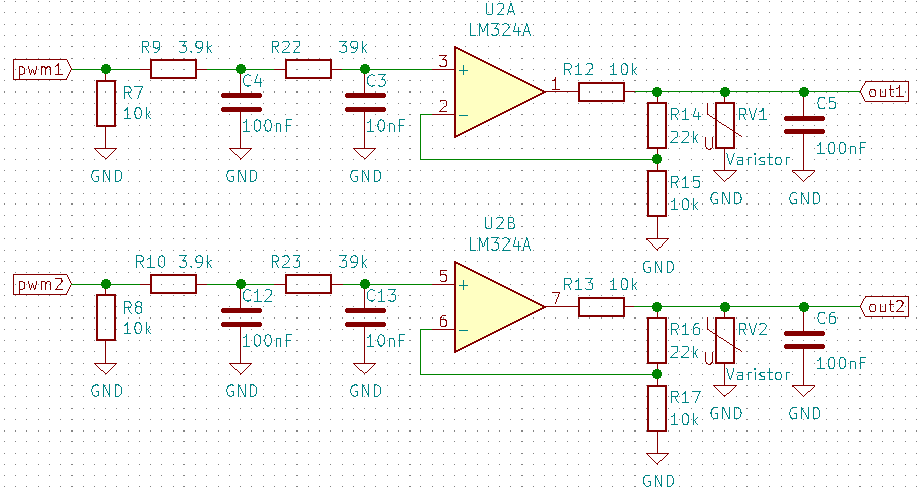
\includegraphics[width=0.8\textwidth]{graphics/shematics_aktor_output.png}
	\caption{10\,V Ausgänge des Aktorbausteins}
	\label{pic: Output_aktor}
\end{figure}
\newpage
\subsubsection{Spannungsversorgung}
Mithilfe eines üblichen $24\;V$ Netzgerätes, welches einen Zylinderstecker 2.1 x 5.5 $mm$ (engl. DC Barrel Jack) hat, kann der Aktorbaustein betrieben werden. So gibt z.B von XP-Power ein $18\;W$  $24\;V/DC$ Netzgerät für 11.73 CHF bei mouser. Um die Logik zu betreiben werden jedoch $3.3\;V$ benötigt. Hier kommt der Spannungswandler MIC4680 zum Einsatz, welcher eine Effizienz von bis zu 90 \% aufweist. Vom Wandler Ausgegeben werden typischerweise $3.3\;V$, im aller schlimmsten Fall kann die Spannung jedoch zwischen $3.201\;V$ und $3.399\;V$ liegen. In der Abbildung \ref{pic: Versorgung_aktor} ist das Schema der $3.3\;V$ Spannungsversorgung zu erkennen, es wurde hier noch eine Sicherung eingebaut da der Print nicht zerstört wird, falls zu viel Strom fliesst. Der Schraubklemmen sind dafür da, um z.B einen ON-OFF-Wippschalter, welcher am Gehäuse montiert wird, anzuschliessen. Die Beschaltung um den Spannungswandler ist dem Datenblatt des MIC4680 zu entnehmen.
\begin{figure}[h!]
	\centering
	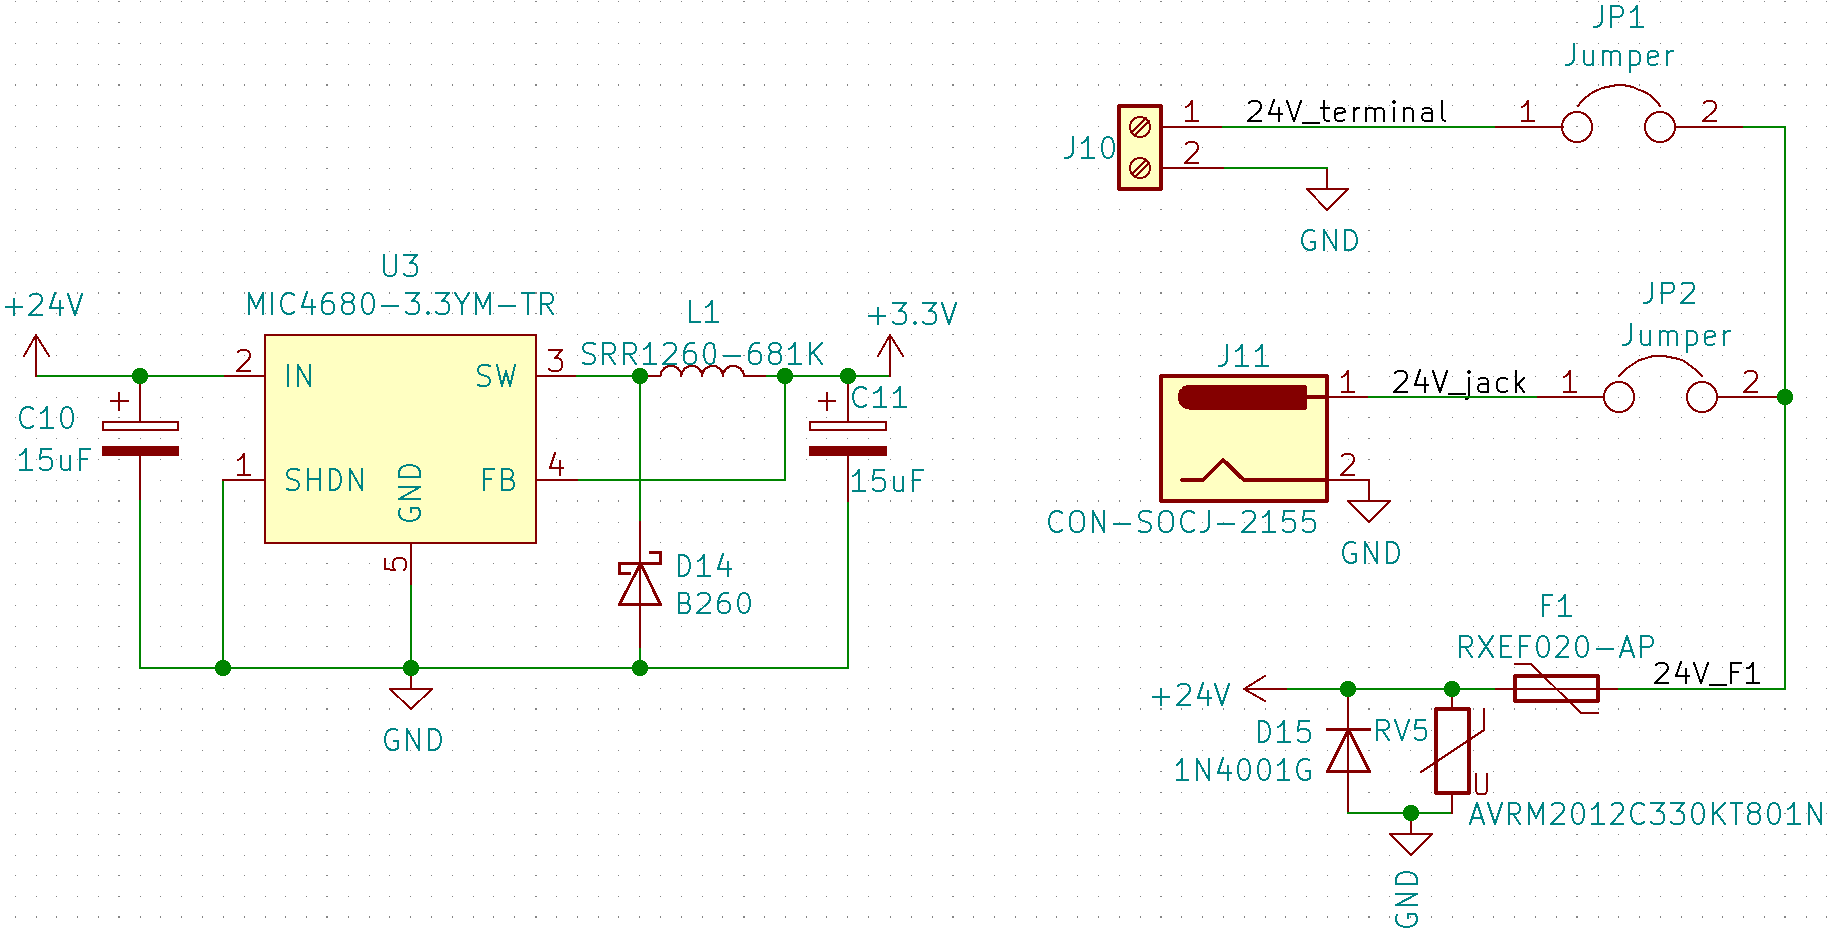
\includegraphics[width=0.7\textwidth]{graphics/shematics_aktor_33V.png}
	\caption{Spannungsversorgung Aktorbaustein}
	\label{pic: Versorgung_aktor}
\end{figure}
\newpage
\subsubsection{Interface}
Die Ausgänge der Relais sowie die 10 $V$ Ein- und Ausgänge sind auf Schraubklemmen geführt (Abb. \ref{pic: Klemmen_aktor}). Es stehen insgesamt 6 LEDs zur Verfügung (Abb. \ref{pic: Buttons_LEDs_aktor}). Die LEDs 1 bis 4 zeigen an ob das jeweilige Relais geschaltet hat. LED5 kann als Status LED verwendet werden. Die Buttons sind die gleichen wie im Sensorbaustein unter Punkt \ref{par: Programmieranschluss} Programmieranschluss.
\begin{figure}[htb]
	\centering
	\begin{minipage}[t]{0.45\linewidth}
	\centering
	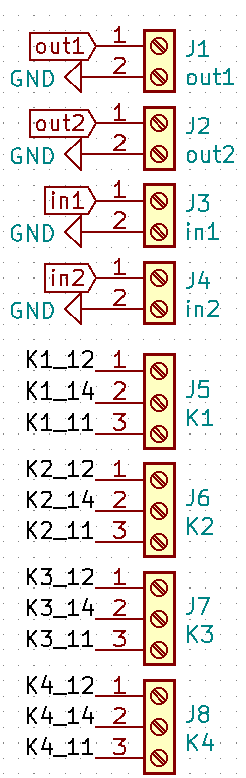
\includegraphics[width=0.35\textwidth]{graphics/shematics_aktor_klemmen.png}
	\caption{Klemmenanschlüsse Aktorbaustein}
	\label{pic: Klemmen_aktor}
	\end{minipage}% <- sonst wird hier ein Leerzeichen eingefügt
	\hfill
	\begin{minipage}[t]{0.45\linewidth}
	\centering
	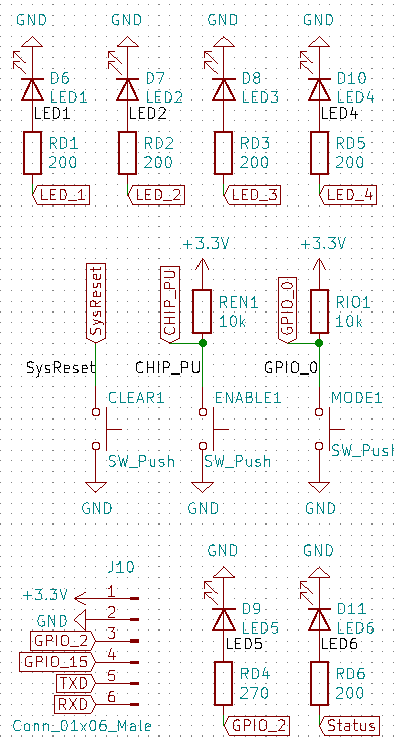
\includegraphics[width=0.9\textwidth]{graphics/shematics_aktor_buttons_LEDs.png}
	\caption{Buttons und LEDs Aktorbaustein}
	\label{pic: Buttons_LEDs_aktor}
	\end{minipage}
\end{figure}


\section{Schluss}

\subsection{Reflektion}

In diesem Kapitel werden die Projekt Ziele Reflektiert. In der untenstehenden Tabelle \ref{tab: Teilziele} sind die zu beginn des Projekts Definierten Teilziele so wie der Status, in welchem der Fachbericht am ende verfasst wurde.
\begin{table}[h!]
	\small
	\begin{tabular}{|c|l|c|}
		\hline 
		Definition & Status \\ 
		\hline 
		Sensor- und Aktorbaustein sind als Prototypen hergestellt& Erfüllt \\ 
		\hline 
		Analyse und Evaluation Mikrocontroller & Erfüllt \\ 
		\hline 
		Frameware ist kompilierbar und erlaubt eine Inbetriebnahme der Prototypen & Erfüllt \\ 
		\hline 
		Signalverknüpfungen sind mit OpenHab realisierbar & Erfüllt \\ 
		\hline 
		Sensor- und Aktorbaustein sind optimiert (Redesign), Mechanisches Gehäuse ist erstellt  & Erfüllt \\ 
		\hline 
		Systemeinrichtung gestaltet sich Benutzerfreundlich & Erfüllt \\ 
		\hline 
		Validierung des gesamten Systems, Testergebnisse sind Dokumentiert n & Erfüllt \\ 
		\hline 
		Befehle können mit Sprachsteuerung ausgeführt werden & Erfüllt \\ 
		\hline 
		Dokumentation abgeschlossen & Erfüllt \\ 
		\hline 
		\end{tabular}
	\caption{Teilziele}
	\label{tab: Teilziele}	 
\end{table}



\subsubsection{Fazit}
 In diesem Projekt wurden Erfahrungen gewonnen, wie eine Hardware Lösung für eine IOT-Anwendung aussehen kann. Es gab einige Probleme wegen des verwendeten Mikrocontrollers, insbesondere des ADCs. Es wurde darauf verzichtet einen externen ADC zu verwenden und andere Lösungen gesucht, sowie die möglichen Verbesserungen der momentanen Lösung erarbeitet. Es hat sich darüber als schwierig herausgestellt, die Temperatur exakt zu messen, da die Umgebungsbedingungen anders sein können, wie stehende Luft und erwärmende Frontplatte. Weitere Erkenntnisse wurden ebenfalls im Bereich des Google Assistent gewonnen, durch die dynamische DNS Adresse  und SSL-Zertifikate gestaltete sich die Integration nicht mit einer direkten Verbindung, siehe Kapitel Sprachassistent.


\section{Ehrlichkeitserklärung}

Hiermit erklären wir, dass die vorliegende Arbeit selbständig von uns, ohne Hilfe Dritter und nur unter Benutzung der angegebenen Quellen verfasst wurde.\\
\\
\\
\\
\\
\\
\\

	\begin{tabular}{l l}
	\textbf{Projekt Team} \\
	\\
	\\
	Lukas Meienberger und Gabriel Nussbaumer \\ 
	\\
	\\
		\rule{44mm}{.15mm} & \hspace{1mm} \rule{70mm}{.15mm} \\
	Ort, Datum & \hspace{1mm} Unterschriften \\
	
\end{tabular}\\


%%---BIBLIOGRAPHY------------------------------------------------------------------------
{\sloppypar
\printbibliography[heading=bibintoc]
}

%%---APPENDIX----------------------------------------------------------------------------
%\begin{appendix} %Anhang
	\section{Anhang Benutzerhandbuch}

%\includepdf[pages={1-2},nup=1x2,landscape=true,scale=0.85,offset=10 -40,pagecommand={\section{Eingefügtes Dokument; zwei Seiten auf einer}\label{app:Aufgabenstellung}\thispagestyle{myheadings}}]{appendix/aufgabenstellung.pdf} \newpage

%%Bei mehrseitigen Dokumenten die folgenden Seiten ohne Überschrift:
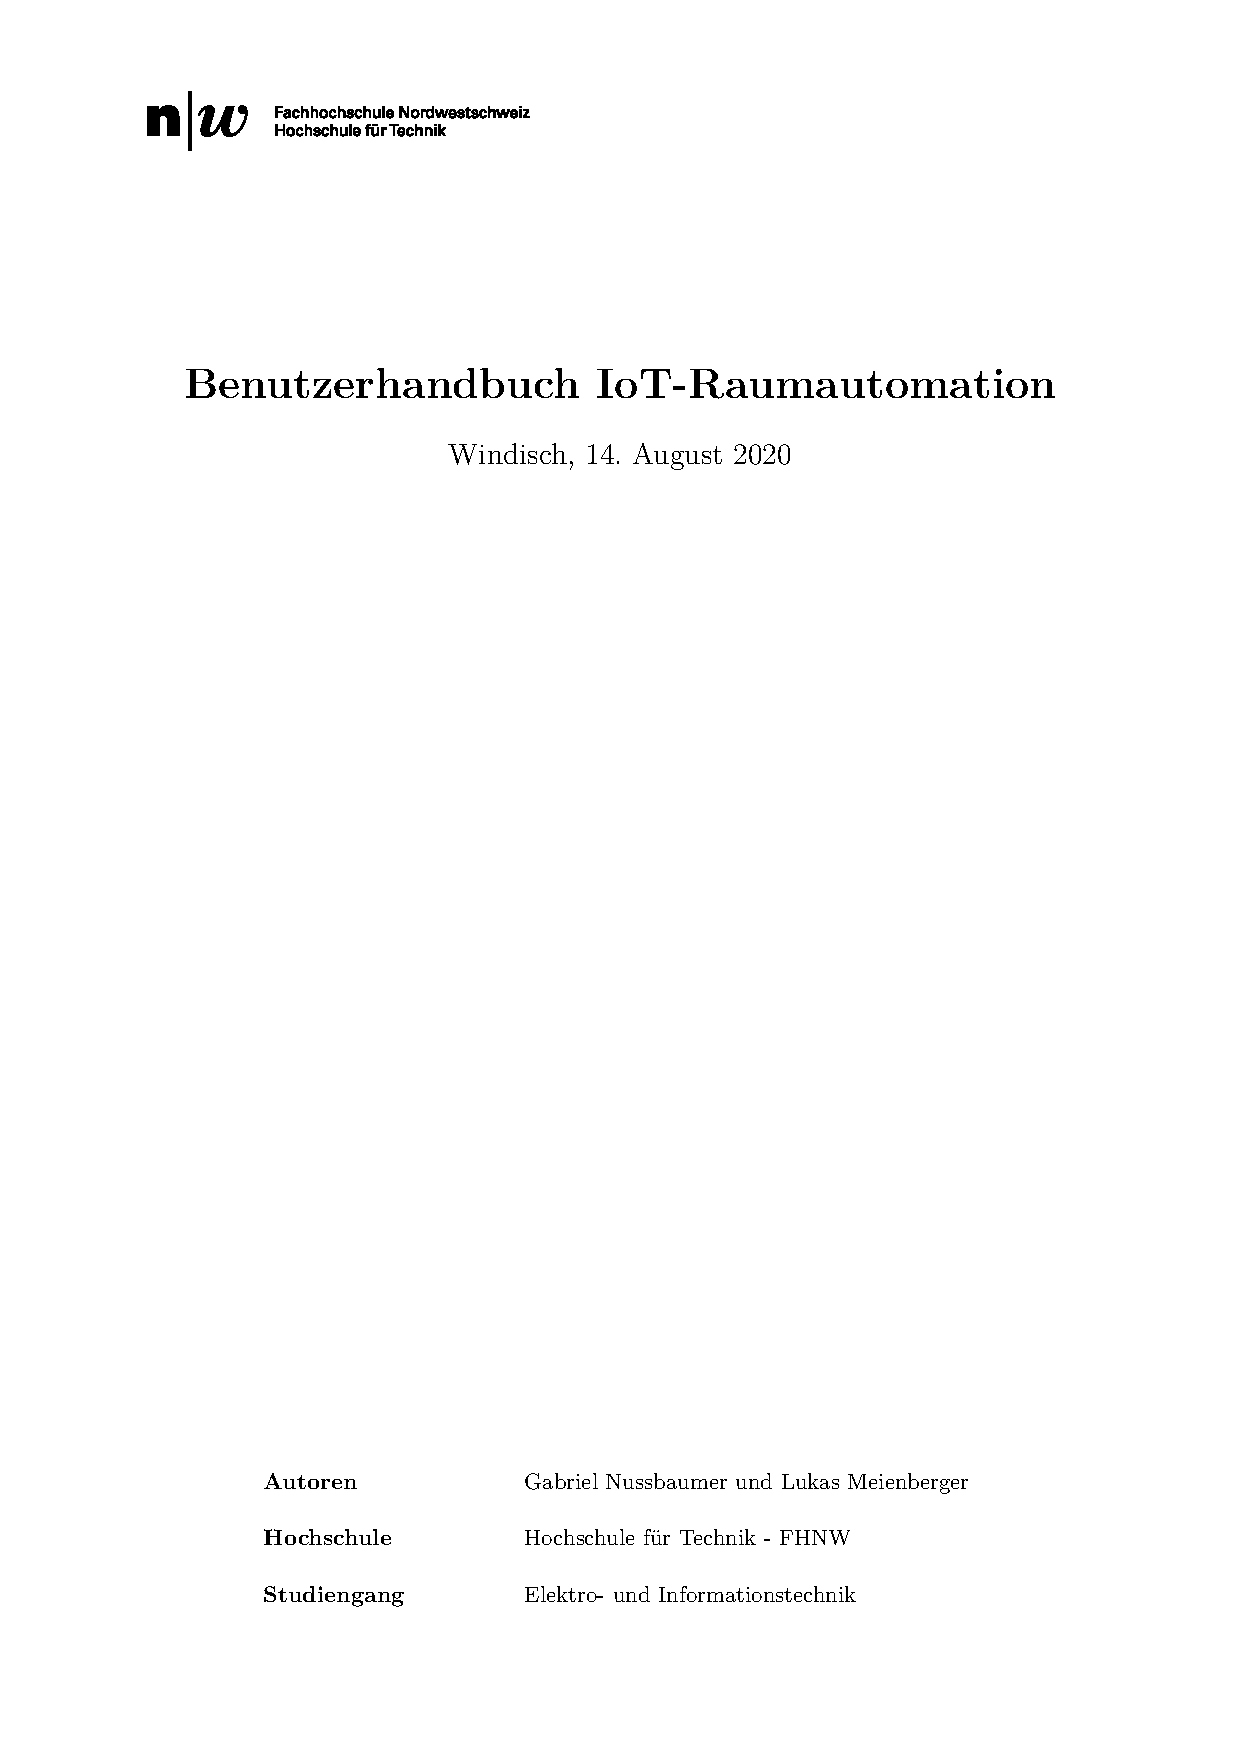
\includepdf[pages=-]{Benutzerhanndbuch.pdf} \newpage

%\includepdf[pages={1},nup=1x1,landscape=true,scale=0.85,offset=10 -40,pagecommand={\section{Eingefügte PDF-Tabelle}\label{app:Timetable}\thispagestyle{myheadings}}]{appendix/timeline_example.pdf} \newpage

%%Bei mehrseitigen Dokumenten die folgenden Seiten ohne Überschrift:
%\includepdf[pages={2-5},nup=1x1,landscape=true,scale=0.85,offset=0 -20,pagecommand={\thispagestyle{myheadings}}]{appendix/timeline_example.pdf} \newpage

\end{appendix}


%%---NOTES for DEBUG---------------------------------------------------------------------
%\newpage
%\listoftodos[\section{Todo-Notes}]
%\clearpage

\end{document}